%%\documentclass[12pt,russianb]{report}
%\usepackage[russian]{babel}
%\usepackage[cp1251]{inputenc}

\documentclass{report}
\usepackage{cmap}
\usepackage[T2A]{fontenc}

\usepackage[utf8]{inputenc}
\usepackage[english,russian]{babel}

\usepackage{longtable}   % подключение длинных таблиц
\usepackage[dvipsnames]{xcolor}
\usepackage{multirow}
\usepackage{array}
\usepackage{indentfirst} % идентификация первых абзацев после секционирования
\usepackage{lastpage}    % пакет достчета страниц 

\usepackage{fancyhdr}                    % расширенный формат страниц
\voffset=-25mm   % -25                   % сдвиг страницы вверх
\hoffset=-15mm   % -10     


  \usepackage[pdftex]{graphicx}            % загрузка графики под pdf
  \usepackage{cmap}                        % чтоб работал поиск по PDF 
  \usepackage[unicode, pdftex, colorlinks, linkcolor=blue]{hyperref}   % гиперссылки в PDF
  \pdfcompresslevel=9                      % сжимаем PDF 
  \textheight=240mm                        % для PDF высота печатного текста
  \textwidth=165mm                         % ширина печатного текста
  \renewcommand{\baselinestretch}{1.3}        % для PDF интервалы между
  \baselineskip=1.3\baselineskip              % строками 


\pagestyle{empty}
\pagestyle{fancy}
\lhead{\tiny ООО <<Опти-Софт>>}
\chead{}
\rhead{\tiny Отчет по обследованию производства \FIRMA}
\cfoot{\rule{\textwidth}{0.25pt}
~\arabic{page}}

\sloppy                             % подавление дополнительных переносов
\righthyphenmin=2                   % можно переносить
\setlength{\parindent}{10mm}        % отступ красной строки

\usepackage{todonotes}
%\newcommand{\todo}[1]{}
%\renewcommand{\todo}[1]{{\color{red} TODO: {#1}}}



\usepackage{placeins}    % пакет позволяет вставлять плавающие объекты (рисунки) в том месте, 
                         % где это необходимо. Для вывода рисунка после него встаить команду \FloatBarrier
                         
                         
                         

\newcommand{\red}[1]{\textcolor{Red}{#1}}
\newcommand{\green}[1]{\textcolor{Green}{#1}}
\newcommand{\blue}[1]{\textcolor{Blue}{#1}}                       
%
\newpage

\chapter{Описание бизнес-архитектуры}

\section{Оргструктура предприятия}

Организационная структура представлена на рис. \ref{pic:Структура.jpg}.

% % Table generated by Excel2LaTeX from sheet 'Лист1'
% \scriptsize
% \begin{longtable}{|p{30mm}|p{90mm}|c|}
% \hline
% {\it {\bf \parbox[c][17mm]{30mm}{\raggedleftАдминистративно-управленческий персонал}}} & {\parbox[c]{90mm}{Генеральный директор}} & \parbox[c]{16mm}{\centering1} \\
% \hline
% \parbox[c][7mm]{30mm}{} & Коммерческий директор &          1 \\
% \hline
% \parbox[c][7mm]{30mm}{} & Финансовый директор &        0,5 \\
% \hline
% \parbox[c][7mm]{30mm}{} & Секретарь руководителя &        0,5 \\
% \hline
% \parbox[c][7mm]{30mm}{} & Юрисконсульт &          1 \\
% \hline
% \parbox[c][7mm]{30mm}{} & Водитель автомобиля &          1 \\
% \hline
% \parbox[c][14mm]{30mm}{} & Инженер по охране труда и промышленной безопасности &          1 \\
% \hline
% \parbox[c][14mm]{30mm}{} & Инженер по гражданской обороне и чрезвычайным ситуациям &        0,5 \\
% \hline
% {\bf \parbox[c][7mm]{30mm}{}} & {\it {\bf Итого}} & {\it {\bf 6,5}} \\
% \hline
% {\it {\bf \parbox[c][7mm]{30mm}{Отдел кадров}}} & Начальник отдела кадров &      0,375 \\
% \hline
% {\it {\bf \parbox[c][7mm]{30mm}{}}} & Специалист по кадрам &          1 \\
% \hline
% {\it {\bf \parbox[c][14mm]{30mm}{}}} & Специалист по воинскому учету (Специалист по военно-учетной работе) &       0,25 \\
% \hline
% {\bf \parbox[c][7mm]{30mm}{}} & {\it {\bf Итого}} & {\it {\bf 1,625}} \\
% \hline
% {\it {\bf \parbox[c][7mm]{30mm}{Бухгалтерия}}} & Главный бухгалтер &          1 \\
% \hline
% {\it {\bf \parbox[c][7mm]{30mm}{}}} & Заместитель главного бухгалтера &          1 \\
% \hline
% {\it {\bf \parbox[c][14mm]{30mm}{}}} & Заместитель главного бухгалтера по внутреннему аудиту &          1 \\
% \hline
% {\it {\bf \parbox[c][7mm]{30mm}{}}} & Бухгалтер (по материалам) &          1 \\
% \hline
% {\it {\bf \parbox[c][7mm]{30mm}{}}} & Бухгалтер (по реализации) &          1 \\
% \hline
% {\it {\bf \parbox[c][7mm]{30mm}{Бюро по з/плате}}} & Начальник бюро  &          1 \\
% \hline
% {\bf \parbox[c][7mm]{30mm}{}} & {\it {\bf Итого}} & {\it {\bf 6}} \\
% \hline
% {\it {\bf \parbox[c][7mm]{30mm}{Отдел главного технолога}}} & Главный технолог &          1 \\
% \hline
% {\it {\bf \parbox[c][7mm]{30mm}{}}} & Инженер-конструктор &          1 \\
% \hline
% {\it {\bf \parbox[c][7mm]{30mm}{}}} & Художник-конструктор &          1 \\
% \hline
% {\it {\bf \parbox[c][7mm]{30mm}{Участок вырубных форм}}} & Мастер участка &          1 \\
% \hline
% {\it {\bf \parbox[c][7mm]{30mm}{}}} &     Техник &          1 \\
% \hline
% {\it {\bf \parbox[c][7mm]{30mm}{}}} &     Техник &          4 \\
% \hline
% {\bf \parbox[c][7mm]{30mm}{}} & {\it {\bf Итого}} & {\it {\bf 9}} \\
% \hline
% {\it {\bf \parbox[c][7mm]{30mm}{Отдел отгрузки}}} & Начальник отдела &          1 \\
% \hline
% \parbox[c][7mm]{30mm}{} & Ведущий инженер &          1 \\
% \hline
% {\it {\bf \parbox[c][7mm]{30mm}{Участок отгрузки (склад)}}} & Начальник участка &          1 \\
% \hline
% {\it {\bf \parbox[c][7mm]{30mm}{}}} & Заведующий склада готовой продукции &          1 \\
% \hline
% \parbox[c][7mm]{30mm}{} & Старший кладовщик &          4 \\
% \hline
% \parbox[c][7mm]{30mm}{} &  Кладовщик &          7 \\
% \hline
% \parbox[c][7mm]{30mm}{} & Транспортировщик 3р &          7 \\
% \hline
% {\bf \parbox[c][7mm]{30mm}{}} & {\it {\bf Итого}} & {\it {\bf 22}} \\
% \hline
% {\it {\bf \parbox[c][7mm]{30mm}{Отдел продаж}}} & Менеджер по продажам &          4 \\
% \hline
% {\it {\bf \parbox[c][7mm]{30mm}{}}} & Менеджер по продажам &          1 \\
% \hline
% {\it {\bf \parbox[c][7mm]{30mm}{Отдел логистики}}} & Начальник отдела  &          1 \\
% \hline
% {\bf \parbox[c][7mm]{30mm}{}} & {\it {\bf Итого}} & {\it {\bf 6}} \\
% \hline
% {\it {\bf \parbox[c][17mm]{30mm}{Отдел материально-технического снабжения}}} & Ведущий менеджер &          1 \\
% \hline
% {\it {\bf \parbox[c][7mm]{30mm}{}}} &   Менеджер &          1 \\
% \hline
% \parbox[c][7mm]{30mm}{} & Заведующий складом &          1 \\
% \hline
% {\bf \parbox[c][7mm]{30mm}{}} & {\it {\bf Итого}} & {\it {\bf 3}} \\
% \hline
% {\it {\bf \parbox[c][11mm]{30mm}{Отдел технического контроля}}} & Начальник отдела &          1 \\
% \hline
% \parbox[c][14mm]{30mm}{} & Старший контролер качества продукции и технологического процесса &          1 \\
% \hline
% \parbox[c][14mm]{30mm}{} & Контролер качества продукции и технологического процесса &          6 \\
% \hline
% {\bf \parbox[c][7mm]{30mm}{}} & {\it {\bf Итого}} & {\it {\bf 8}} \\
% \hline
% {\it {\bf \parbox[c][11mm]{30mm}{Отдел главного энергетика}}} & Главный энергетик-начальник отдела &          1 \\
% \hline
% \parbox[c][14mm]{30mm}{} & Заместитель главного энергетика по автоматизации производства &          1 \\
% \hline
% \parbox[c][7mm]{30mm}{} & Инженер-электроник &          1 \\
% \hline
% \parbox[c][7mm]{30mm}{} &    Инженер &        0,5 \\
% \hline
% \parbox[c][14mm]{30mm}{} & Электромонтер по ремонту и обслуживанию электрооборудования 5р &          1 \\
% \hline
% \parbox[c][14mm]{30mm}{} & Электромонтер по ремонту и обслуживанию электрооборудования 6р &          1 \\
% \hline
% \parbox[c][14mm]{30mm}{} & Электромонтер по ремонту и обслуживанию электрооборудования 6р &          3 \\
% \hline
% \parbox[c][7mm]{30mm}{} & Слесарь-ремонтник 5р &          1 \\
% \hline
% \parbox[c][7mm]{30mm}{} & Слесарь-ремонтник 6р &          1 \\
% \hline
% \parbox[c][7mm]{30mm}{} & Слесарь-ремонтник 6р &          1 \\
% \hline
% {\bf \parbox[c][7mm]{30mm}{}} & {\it {\bf Итого}} & {\it {\bf 11,5}} \\
% \hline
% {\it {\bf \parbox[c][7mm]{30mm}{Отдел главного механика}}} & Главный механик &          1 \\
% \hline
% {\it {\bf \parbox[c][7mm]{30mm}{}}} &    Механик &          1 \\
% \hline
% {\it {\bf \parbox[c][7mm]{30mm}{}}} & Слесарь-ремонтник 5р &          8 \\
% \hline
% \parbox[c][7mm]{30mm}{} & Слесарь-ремонтник 6р &          1 \\
% \hline
% \parbox[c][7mm]{30mm}{} & Слесарь-ремонтник 6р &          3 \\
% \hline
% {\bf \parbox[c][7mm]{30mm}{}} & {\it {\bf Итого}} & {\it {\bf 14}} \\
% \hline
% {\it {\bf \parbox[c][14mm]{30mm}{Производство гофрокартона}}} & Заместитель генерального директора по производству &          1 \\
% \hline
% {\it {\bf \parbox[c][7mm]{30mm}{}}} & Начальник производства &          1 \\
% \hline
% {\it {\bf \parbox[c][7mm]{30mm}{}}} & Инженер по оборудованию &          1 \\
% \hline
% {\it {\bf \parbox[c][7mm]{30mm}{}}} &    Инженер &          1 \\
% \hline
% {\it \parbox[c][17mm]{30mm}{Бюро планирования и подготовки производства}} & Начальник бюро &          1 \\
% \hline
% {\it \parbox[c][7mm]{30mm}{}} & Инженер-экономист &          1 \\
% \hline
% {\it \parbox[c][7mm]{30mm}{}} & Инженер-экономист &          1 \\
% \hline
% {\it \parbox[c][7mm]{30mm}{}} & Техник по учету &          1 \\
% \hline
% {\it \parbox[c][7mm]{30mm}{Участок гофрокартона}} & Сменный мастер &          4 \\
% \hline
% {\it \parbox[c][7mm]{30mm}{}} & Машинист гофрировального агрегата 5р &          4 \\
% \hline
% {\it \parbox[c][7mm]{30mm}{}} & Машинист гофрировального агрегата 5р &          5 \\
% \hline
% {\it \parbox[c][7mm]{30mm}{}} & Машинист гофрировального агрегата 4р &          2 \\
% \hline
% {\it \parbox[c][7mm]{30mm}{}} & Машинист гофрировального агрегата 3р &          7 \\
% \hline
% {\it \parbox[c][14mm]{30mm}{}} & Съемщик целлюлозы, бумаги, картона и изделий из них 2р &          4 \\
% \hline
% {\it \parbox[c][7mm]{30mm}{}} & Клеевар 3р &          1 \\
% \hline
% {\it \parbox[c][7mm]{30mm}{}} & Машинист печатно-высекального агрегата 5р &          5 \\
% \hline
% {\it \parbox[c][7mm]{30mm}{}} & Машинист печатно-высекального агрегата 5р &          9 \\
% \hline
% {\it \parbox[c][7mm]{30mm}{}} & Машинист печатно-высекального агрегата 4р &          2 \\
% \hline
% {\it \parbox[c][7mm]{30mm}{}} & Машинист печатно-высекального агрегата 3р &          1 \\
% \hline
% {\it \parbox[c][7mm]{30mm}{}} & Укладчик-упаковщик 3р &          4 \\
% \hline
% {\it \parbox[c][7mm]{30mm}{}} & Укладчик-упаковщик 3р &         36 \\
% \hline
% {\it \parbox[c][7mm]{30mm}{}} & Укладчик-упаковщик 4р &         30 \\
% \hline
% {\it \parbox[c][7mm]{30mm}{}} & Прессовщик отходов 2р &          4 \\
% \hline
% {\it \parbox[c][7mm]{30mm}{}} & Плотник 3р &          4 \\
% \hline
% {\it \parbox[c][14mm]{30mm}{}} & Наладчик оборудования в бумажном производстве &          4 \\
% \hline
% {\it \parbox[c][11mm]{30mm}{Автотранспортный участок}} & Начальник участка &        0,5 \\
% \hline
% {\it \parbox[c][7mm]{30mm}{}} & Водитель автомобиля 4р &          3 \\
% \hline
% {\it \parbox[c][7mm]{30mm}{}} & Водитель погрузчика 5р &         28 \\
% \hline
% {\it \parbox[c][7mm]{30mm}{}} & Слесарь-ремонтник 5р &          4 \\
% \hline
% \parbox[c][5mm]{30mm}{Итого} &            &        257 \\
% \hline

% \caption{Структура штатного расписания}\label{tab:orgchart}
% \end{longtable}  
% \normalsize

% Организационная структура представлена на рис. \ref{pic:structure},  \ref{pic:structure1}.

%\begin{figure}
 %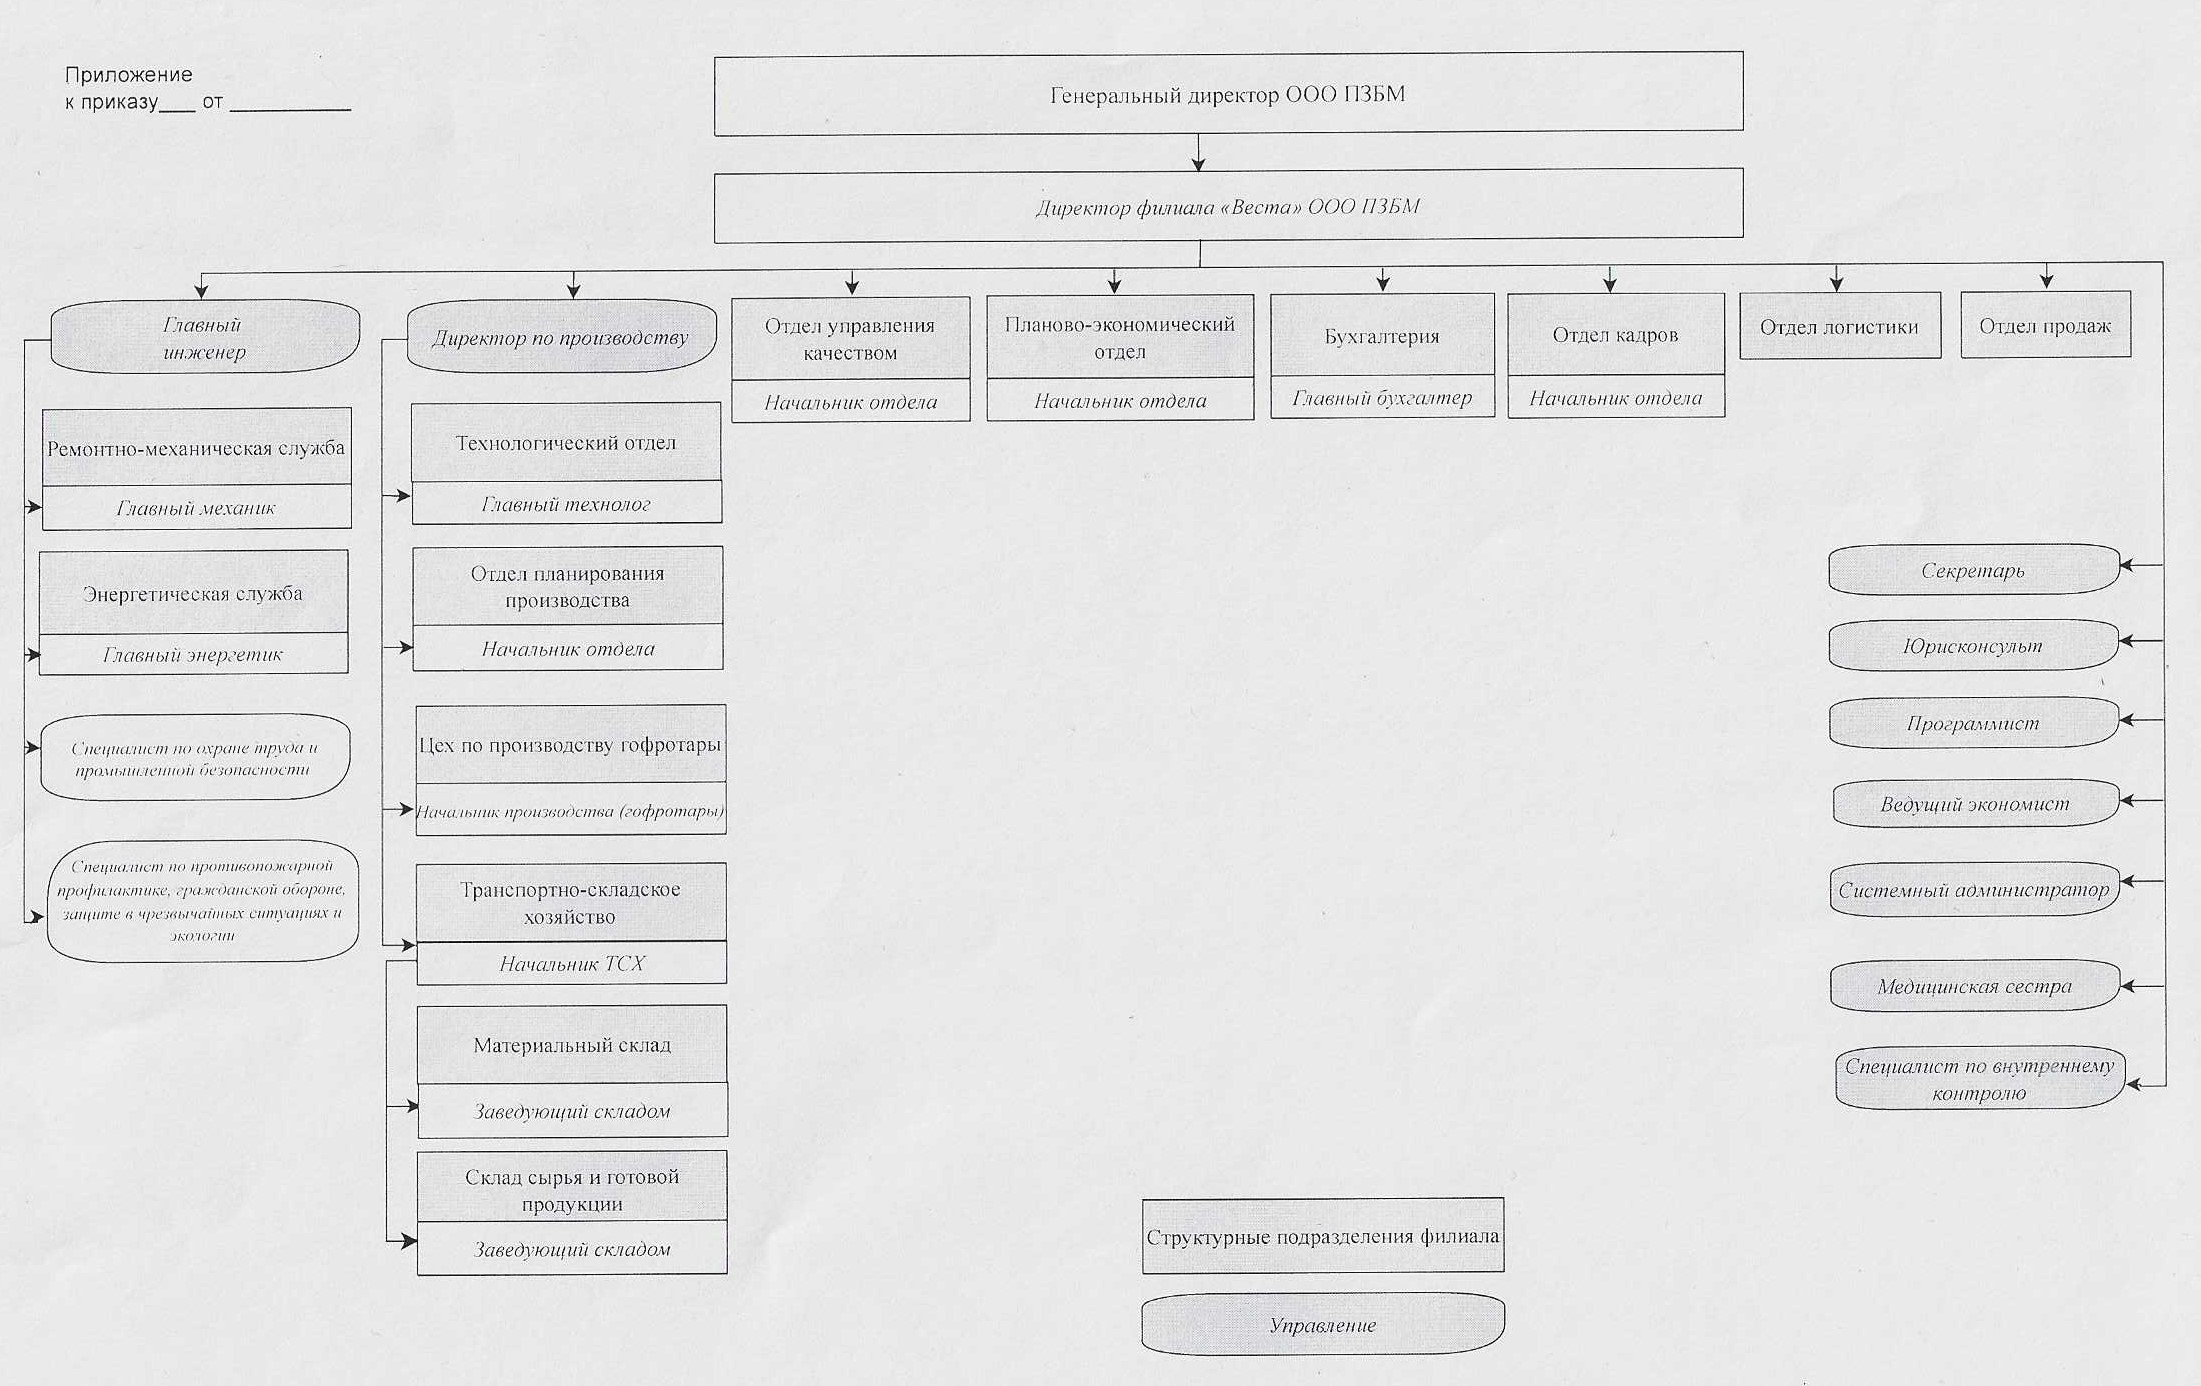
\includegraphics[height=0.94\textheight, keepaspectratio]{Pics/Структура.jpg}
 %\caption{Оргштатная структура \FIRMA}
% \label{pic:Структура.jpg}
%\end{figure}

%\clearpage

\begin{figure}
\begin{center}
  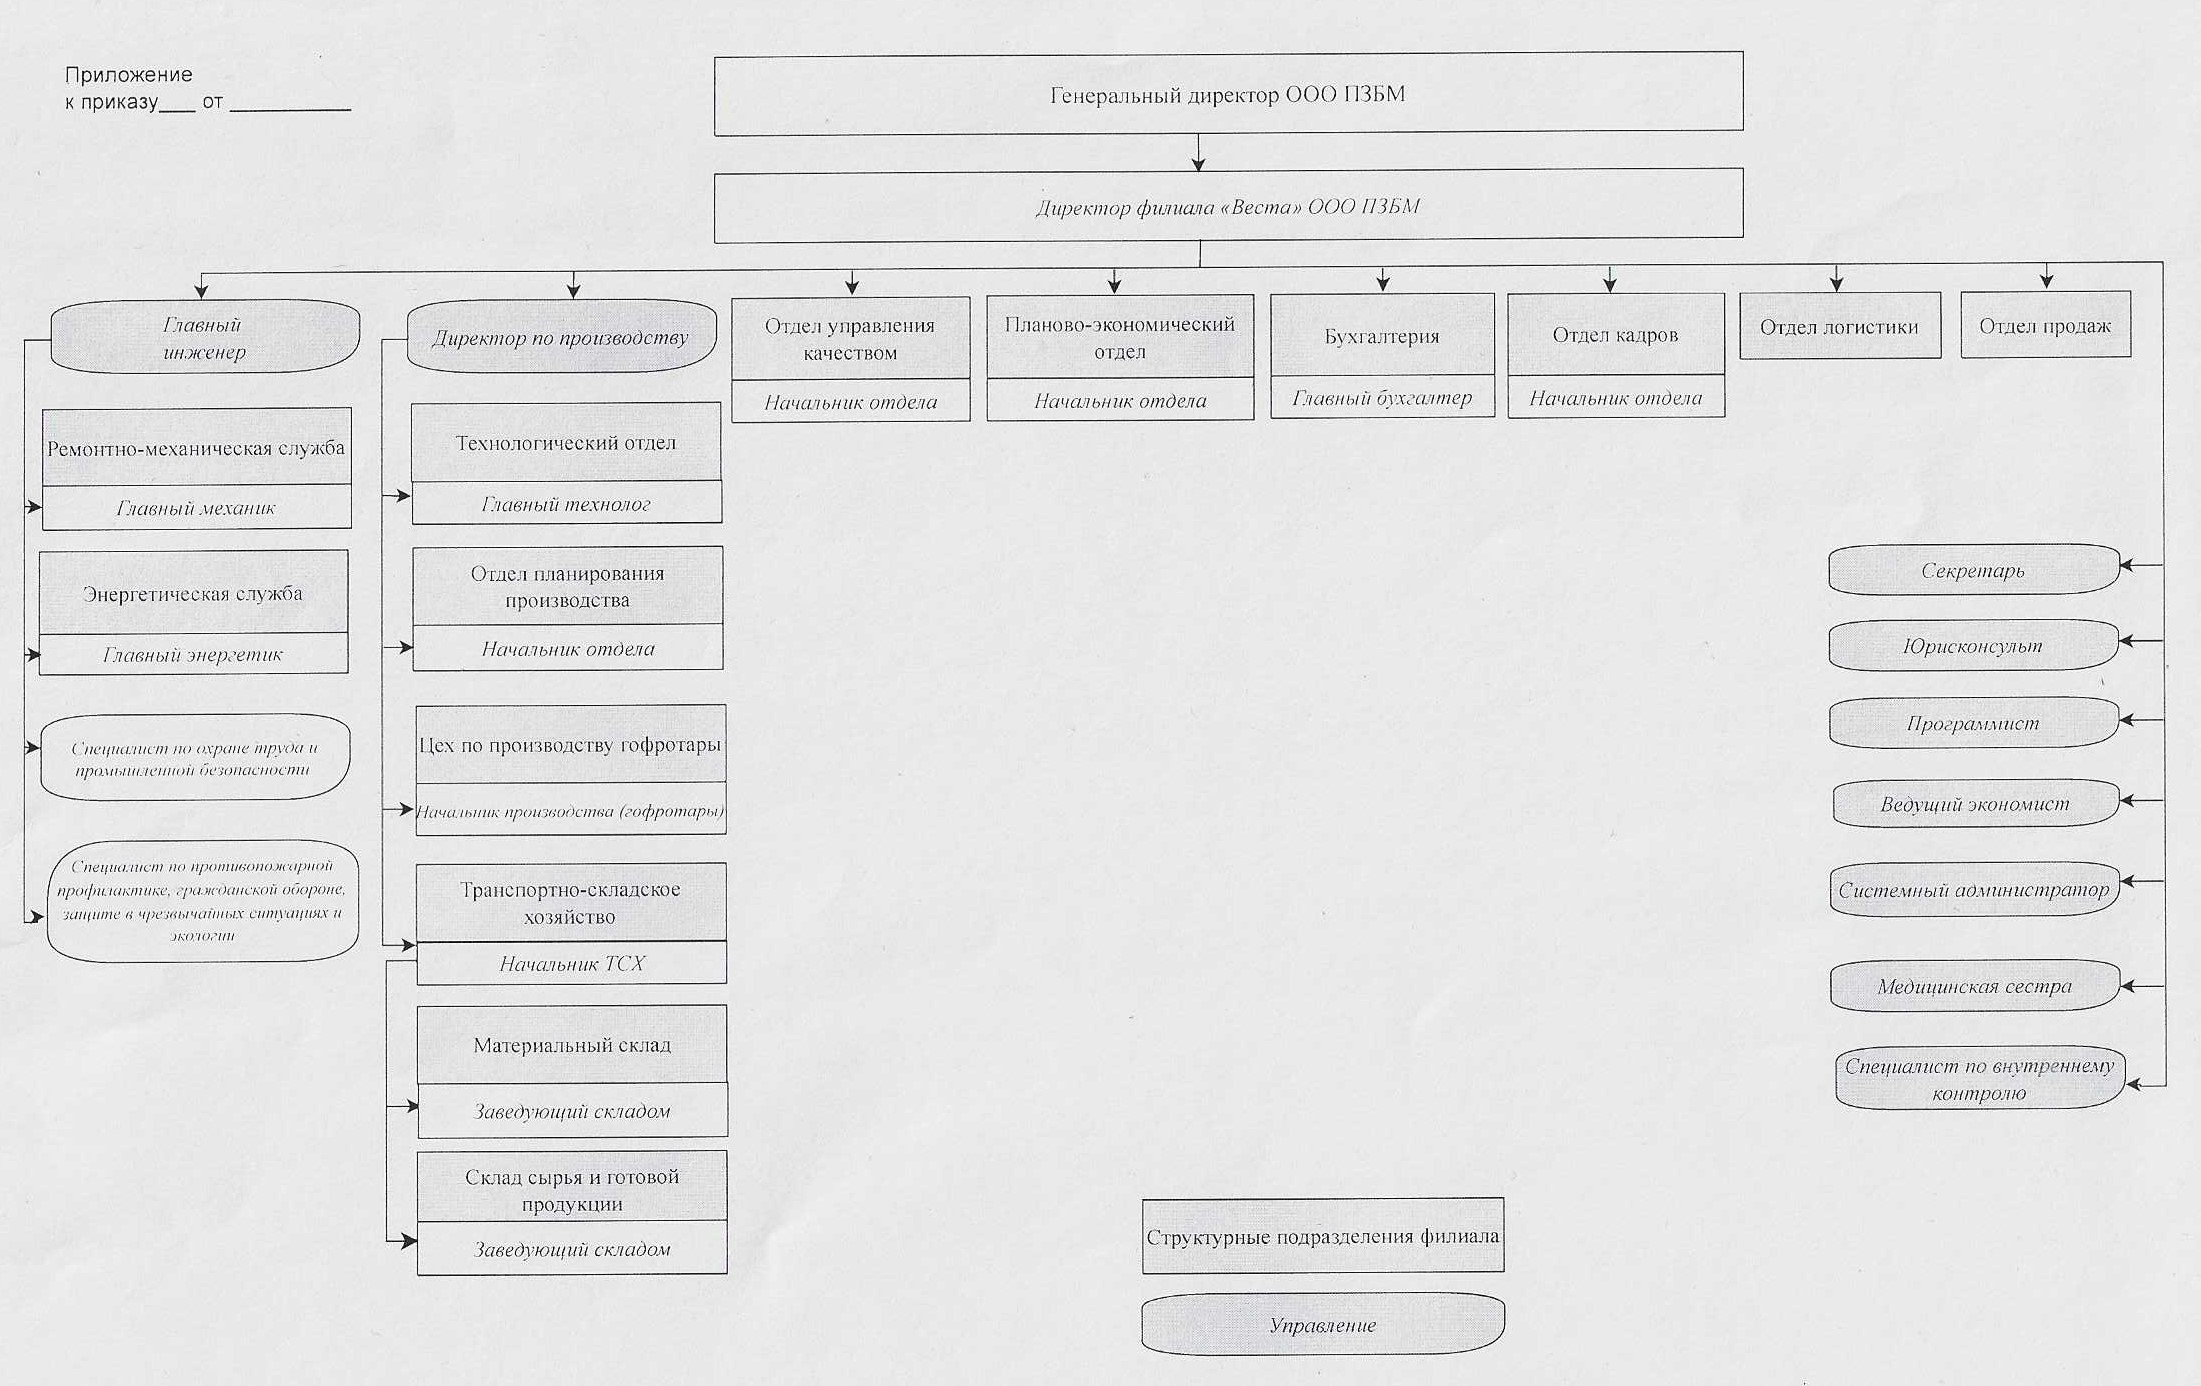
\includegraphics[height=1.2\textheight, width=\textwidth, angle=90, keepaspectratio]{Pics/Структура.jpg}
\end{center}
  \caption{Оргштатная структура. \FIRMA}
  \label{pic:Структура.jpg}
\end{figure}
% \begin{figure}
% \begin{center}
%   \includegraphics[
%   %width=\textwidth, height=1\textheight, 
%   angle=90, keepaspectratio]{Pics/Structure3.png}
% \end{center}
%   \caption{Организационная структура производства. Продолжение}
%   \label{pic:structure}
% \end{figure}
% \clearpage


%%\begin{figure}
%\begin{center}
%\ifnum\pdfoutput=0
%  \includegraphics[40,0][366,292]{Pics/structure.png}
%\else 
%  \includegraphics[height=0.94\textheight, keepaspectratio]{Pics/00_Структура.jpg}
%\fi
%\end{center}
%  \caption{Оргштатная структура АО ''Новосибирский КБК''}
%  \label{pic:structure}
%\end{figure}

\clearpage

\section{Территориальное расположение}
%

Местонахождение ПРЕДПРИЯТИЯ --- \CURADDRESS.

Адрес производства:
\ADDRESS.



\newpage
\section{Описание производственных процессов}

%%\documentclass[12pt,russianb]{report}
%\usepackage[russian]{babel}
%\usepackage[cp1251]{inputenc}

\documentclass{report}
\usepackage{cmap}
\usepackage[T2A]{fontenc}

\usepackage[utf8]{inputenc}
\usepackage[english,russian]{babel}

\usepackage{longtable}   % подключение длинных таблиц
\usepackage[dvipsnames]{xcolor}
\usepackage{multirow}
\usepackage{array}
\usepackage{indentfirst} % идентификация первых абзацев после секционирования
\usepackage{lastpage}    % пакет достчета страниц 

\usepackage{fancyhdr}                    % расширенный формат страниц
\voffset=-25mm   % -25                   % сдвиг страницы вверх
\hoffset=-15mm   % -10     


  \usepackage[pdftex]{graphicx}            % загрузка графики под pdf
  \usepackage{cmap}                        % чтоб работал поиск по PDF 
  \usepackage[unicode, pdftex, colorlinks, linkcolor=blue]{hyperref}   % гиперссылки в PDF
  \pdfcompresslevel=9                      % сжимаем PDF 
  \textheight=240mm                        % для PDF высота печатного текста
  \textwidth=165mm                         % ширина печатного текста
  \renewcommand{\baselinestretch}{1.3}        % для PDF интервалы между
  \baselineskip=1.3\baselineskip              % строками 


\pagestyle{empty}
\pagestyle{fancy}
\lhead{\tiny ООО <<Опти-Софт>>}
\chead{}
\rhead{\tiny Отчет по обследованию производства \FIRMA}
\cfoot{\rule{\textwidth}{0.25pt}
~\arabic{page}}

\sloppy                             % подавление дополнительных переносов
\righthyphenmin=2                   % можно переносить
\setlength{\parindent}{10mm}        % отступ красной строки

\usepackage{todonotes}
%\newcommand{\todo}[1]{}
%\renewcommand{\todo}[1]{{\color{red} TODO: {#1}}}



\usepackage{placeins}    % пакет позволяет вставлять плавающие объекты (рисунки) в том месте, 
                         % где это необходимо. Для вывода рисунка после него встаить команду \FloatBarrier
                         
                         
                         

\newcommand{\red}[1]{\textcolor{Red}{#1}}
\newcommand{\green}[1]{\textcolor{Green}{#1}}
\newcommand{\blue}[1]{\textcolor{Blue}{#1}}                       
\newpage

\subsection{Управление взаимоотношениями с клиентами}
\label{BP_CRM}

Привлечением новых клиентов на ПРЕДПРИЯТИИ занимается отдела продаж.

Менеджеры отдела продаж ищут новых клиентов в различных открытых источниках, через обзвон потенциальных покупателей, через Интернет. 
Менеджеры для поиска новых клиентов используют холодные звонки, выставки, командировки, образцы гофропродукции с полок магазинов. Есть разработанная памятка по общению с потенциальными клиентами (рис. \ref{pic:I.2.jpg}). По факту процесс общения и взаимодействия с потенциальным клиентом менеджер выбирает сам.

Численность отдела продаж на момент обследования составляет 7 человек: 1 руководитель отдела и 6 менеджеров отдела продаж.
Направления продаж распределены между менеджерами следующим образом.

\begin{itemize}
    \item 2 человека работают на рабочих местах. Их направление продаж  ''Калужское направление'', структурно подчиняются ООО ТД ''ФОРМАТ''.
    \item 1 человек исполняет обязанности старшего менеджера. Структурно подчиняется Филиалу «Веста» ООО ''ПЗБМ''. Должностные обязанности включают в себя кроме выполнения продаж, формирование отчетности по запросам ООО ТД ''ФОРМАТ'' и Филиала «Веста» ООО ''ПЗБМ'', участие в планерных и прочих совещаниях, контроль дебиторской задолженности, контроль загруженности склада ГП и т.д.
    \item 1 человек работает удаленно. Физически располагается в городе Москва, структурно подчиняется ООО ТД ''ФОРМАТ''. Направление поиска клиентов - ''Московское направление''.
    \item 2 человека  работают удаленно. Физически располагаются в городе Брянск. Структурно подчиняются ООО ТД ''ФОРМАТ''. Направление поиска клиентов - ''Центральный регион'' и трейдеры, что составляет 10-20 \% от общего объема выпускаемой ПРЕДПРИЯТИЕМ продукции.
    
\end{itemize}


Не смотря на то, что существует распределение по направлениям продаж, соблюдается оно условно.


Системы CRM на предприятии не выявлено. Общей базы новых (потенциальных) клиентов на предприятии не ведется. Аналитики направления развития продаж нет. Каждый менеджер ведет свою базу в удобной для себя форме (рис. \ref{pic:I.3..jpg}). Учет взаимоотношений с клиентами ведется на ручном уровне и в удобной для каждого менеджера форме. Информация по новым клиентам у менеджеров находится только в электронных письмах и личных записях. Опросный лист для клиента не используется, собирается только информация, достаточная, для анализа возможности изготовления на предприятия и быстрого расчета стоимости.   

Почта приходит на общий электронный адрес. 
Звонки и электронная почта поступают лично каждому менеджеру.
Количество новых клиентов примерно 5-6 в месяц.



 

%CRM системы не выявлено.


%Единой базы потенциальных покупателей не выявлено.

%Новых клиентов менеджер заводит в справочник Контрагенты в системе СБИС только при заключении договора.

% Новые клиенты заносятся как лиды. МАП заносит карточку покупателя в модуле CRM системы 1С: УНФ. МАП ведет историю взаимоотношений с клиентами вручную записывая историю звонков, рассылок.
% В CRM созданы шаблоны сценариев работы с покупателем. Каждое событие работы с контрагентом является  элементом справочника с тем  шаблоном.
% При появлении потенциального клиента МАП определяет лицо принимающее решение со стороны организации. МАП запрашивает требования по изготовлению изделия и получает техническое задание (размеры и характеристики нового изделия). 

 %В отделе продаж есть четкий регламент работы по новым заказчикам.
% Одна сделка представляет собой несколько изделий готовой продукции для одного клиента.

%
%
%
%
%%
%Менеджеры отдела маркетинга 
%занимаются поиском и привлечением новых покупателей. Выделяется пассивный поиск через сайт, рекламу и участие в мероприятиях, и активный поиск через адресную рассылку.
%Все контакты хранятся на сетевом ресурсе в сети ПРЕДПРИЯТИЯ, куда есть доступ большинству пользователей сети.
%При появлении нового покупателя менеджеры отдела маркетинга создают каталог в сетевом каталоге клиентов.
%Внутри каталога хранится информация по письмам с клиентами, договорам, спецификациям и тендерам.
%
%%
%Новых заказчиков ведет менеджер отдела продаж и закупок.
%После выполнения предварительных заказов заказчику ведущий специалист отдела продаж передает клиентов менеджерам отдела продаж.
%%
%%\begin{figure}
%%\begin{center}
%%\ifnum\pdfoutput=0
%%  \includegraphics[40,0][366,292]{Pics/TK1.png}
%%\else 
%%  \includegraphics[height=0.94\textheight, keepaspectratio]{Pics/CustomerList.jpg}
%%\fi
%%\end{center}
%%  \caption{Разделение потребителей гофротары в разрезе маркетологов}
%%  \label{pic:CustomerList}
%%\end{figure}
%%\clearpage
%%
%%
\begin{figure}
\begin{center}
 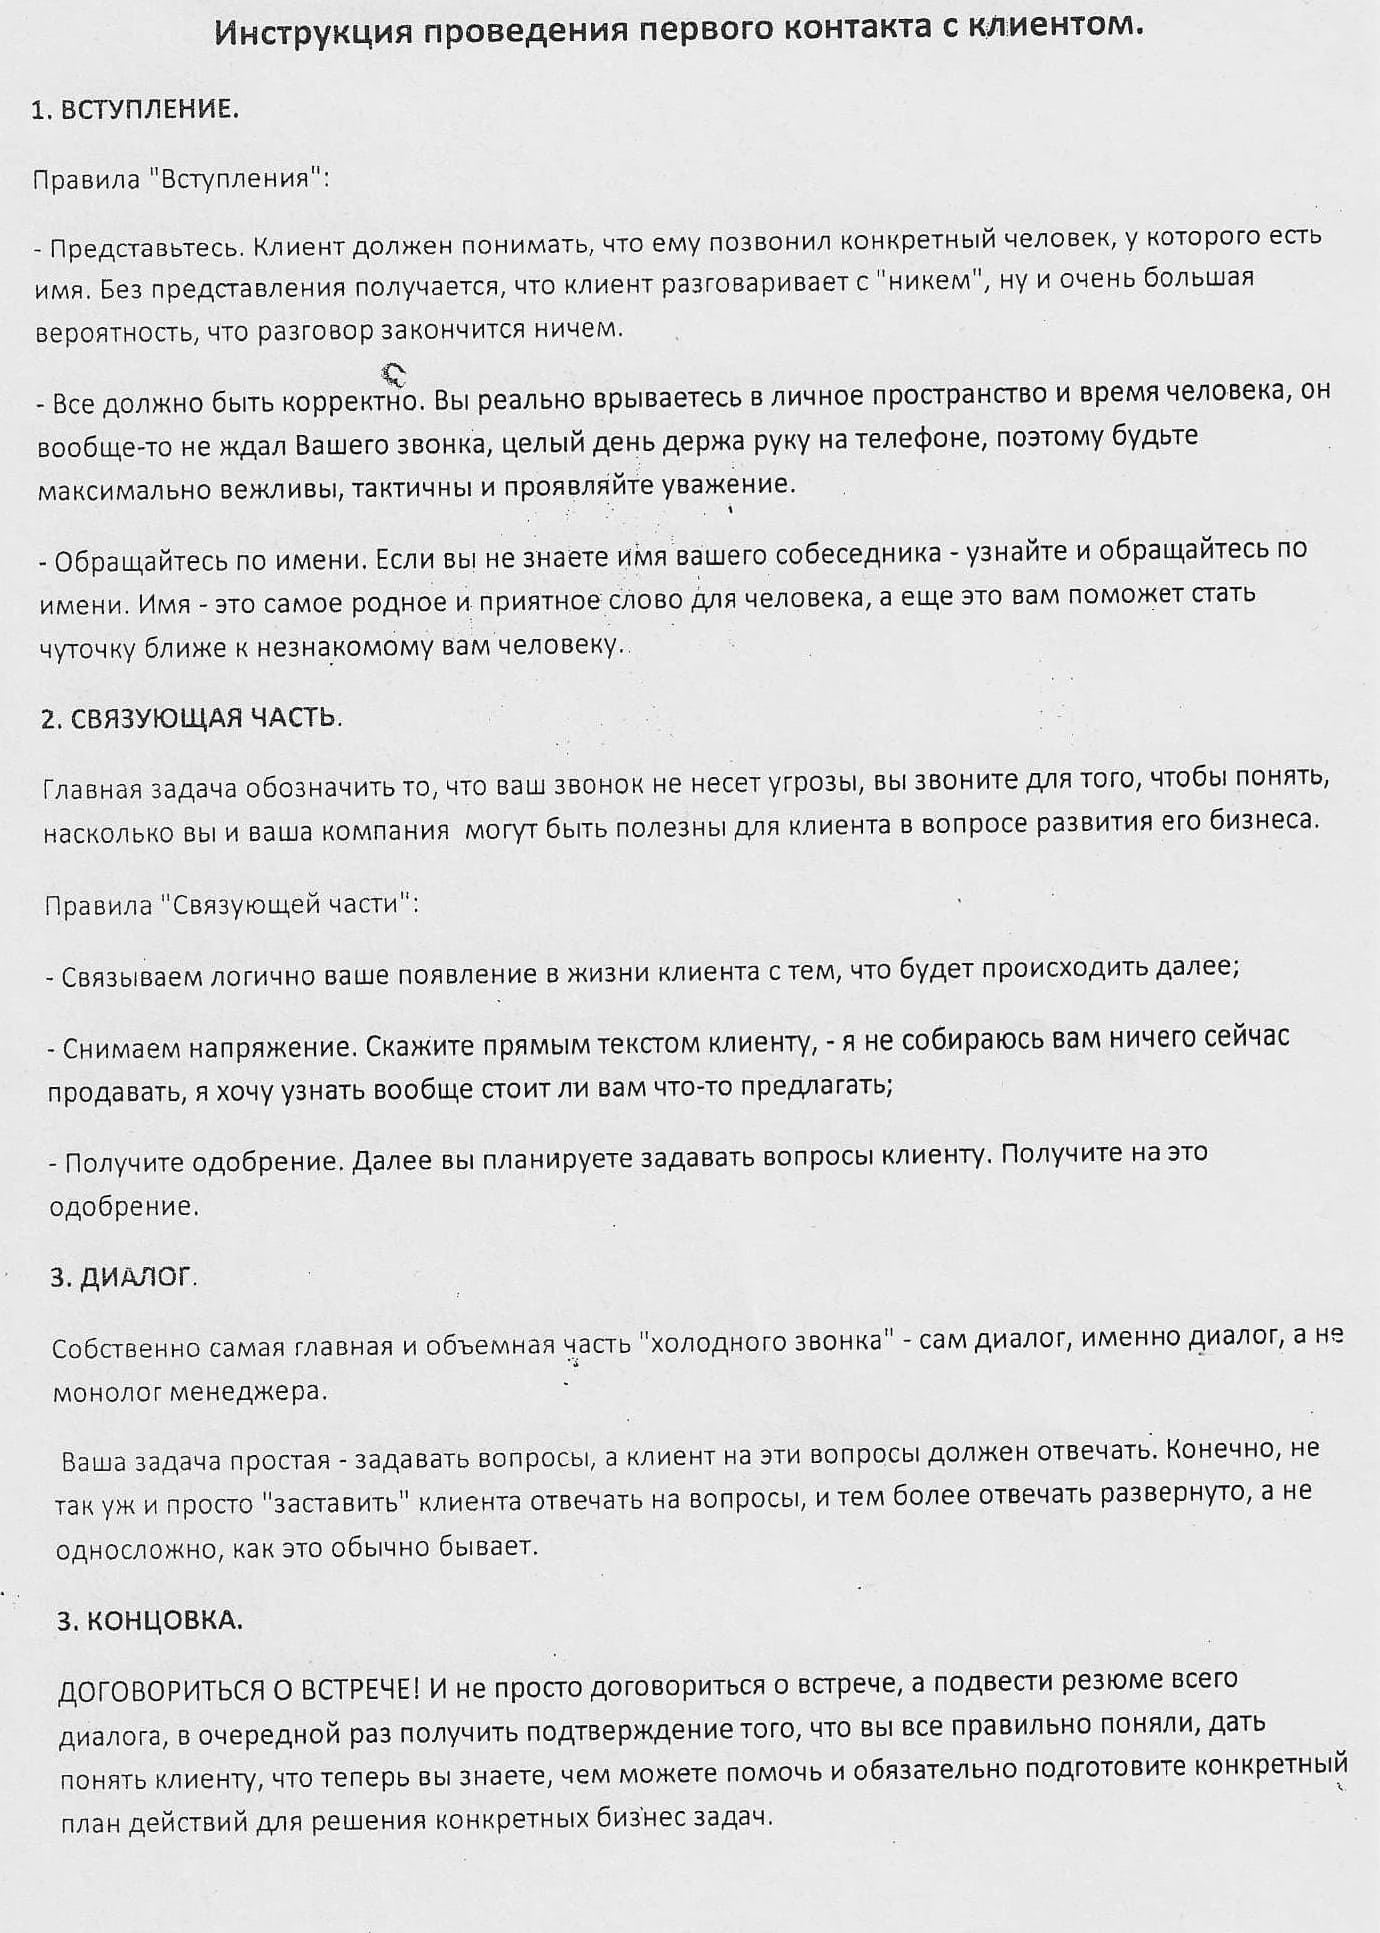
\includegraphics[height=0.8\textheight, keepaspectratio]{Pics/I.2.jpg}
\end{center}
 \caption{Памятка менеджеру}
 \label{pic:I.2.jpg}
\end{figure}
\clearpage

\begin{figure}[!h]
\begin{center}
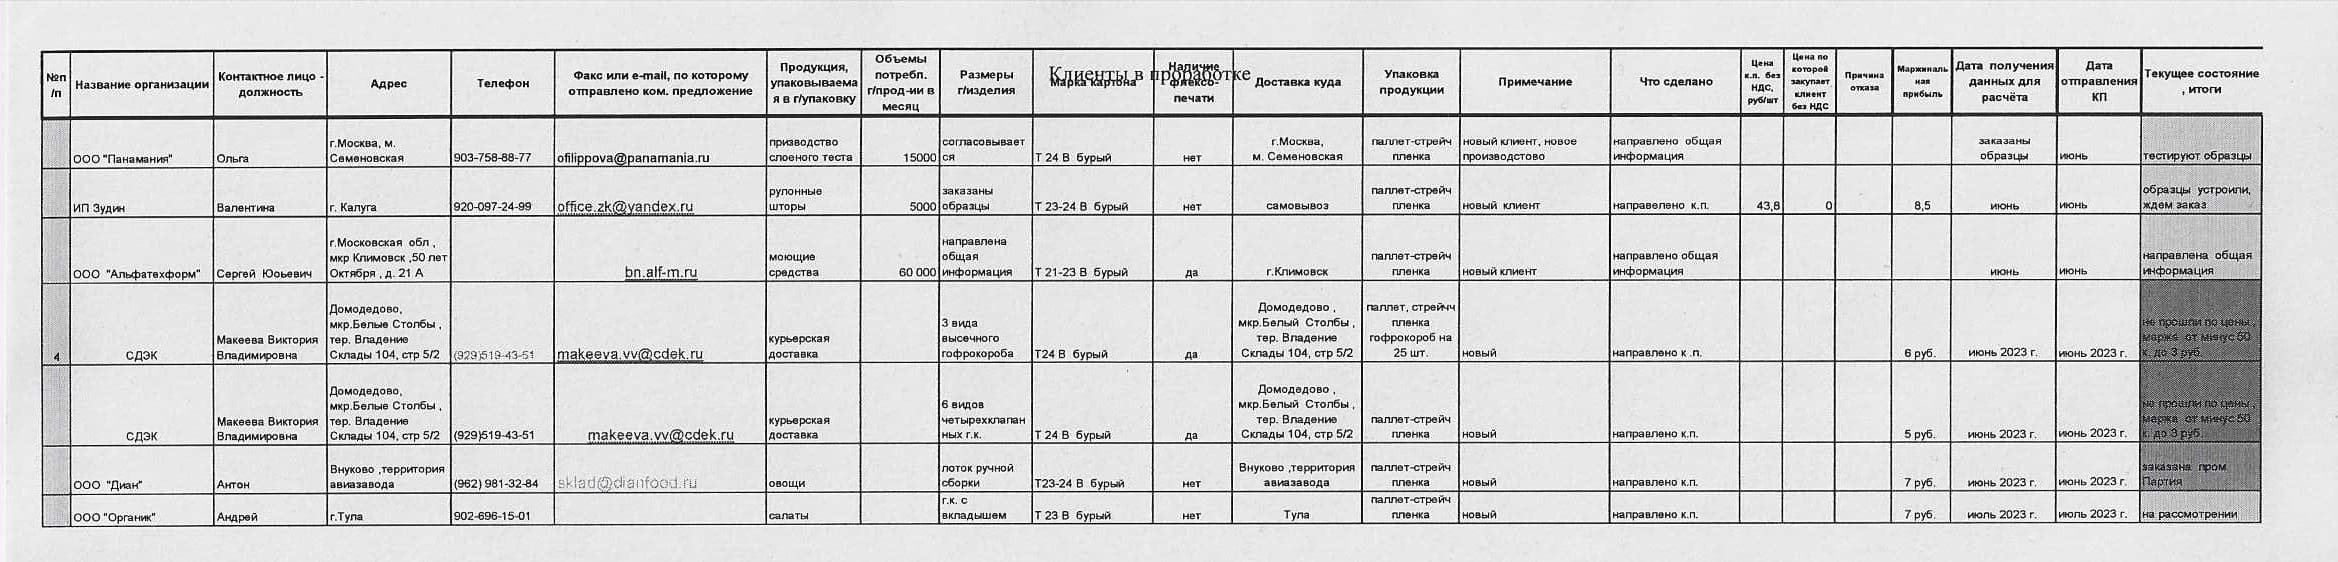
\includegraphics[height=0.3\textheight, width=1.1\textwidth, angle=90, keepaspectratio]{Pics/I.3..jpg}
\end{center}
 \caption{Пример реестра новых (потенциальных) клиентов }
 \label{pic:I.3..jpg}
\end{figure}
\clearpage

%
%
%
%


%\clearpage
\ifx \notincludehead\undefined
\normalsize
\end{document}
\fi 
\newpage
\subsection{Долгосрочное планирование продаж}
\label{bp:monthplan}


Долгосрочным планированием продаж на ПРЕДПРИЯТИИ занимается ООО ТД ''ФОРМАТ''. %заместитель коммерческого директора.
ПРЕДПРИЯТИЕ входит в группу предприятий ''Объединенные бумажные фабрики'', далее по тексту ГП ''ОБФ'' .
Процесс долгосрочного планирования продаж происходит в соответствии с процессами описанными ниже.


  \textbf{Долгосрочное планирование - ''Стратегический план развития на 7 лет''}
    
Формируется стратегический план развития ГП ''ОБФ'' на 7 лет с указанием направлений развития ГП ''ОБФ'', таких как:  постановка новых целей, увеличение объема продаж, модернизация/покупка оборудования и т.д.

  \textbf{Среднесрочное планирование - ''Тактический план развития на 3 года''}
    
Тактическое планирование осуществляется согласно промежуточным стратегическим целям. Включает в себя планы действий и методы реализации стратегии, необходимые для формирования условий деятельности как ГП ''ОБФ'' в целом, так и отдельно каждого предприятия в составе группы.

\textbf{Краткосрочное планирование - ''Оперативный план развития на 1 год''}

Основные задачи краткосрочного планирования: достижение оперативных целей, решение текущих задач ГП ''ОБФ'' и ее структурных подразделений. Планирование предполагает оптимизацию используемых ресурсов. В оперативном планировании учитывается реальное состояние внешней и внутренней среды каждого предприятия в составе ГП ''ОБФ'' в планируемом периоде.
Формирование оперативного плана осуществляет планово-экономическим отдел.  
Внутри ГП ''ОБФ'' для обозначения оперативного плана именуется используется термин ''ПРОФИНТЕХПЛАН'' (форма \ref{pic:XI.1}).

Планово-экономический отдел производит расчет загрузки производственных мощностей по каждой единице оборудования с учетом графика работы предприятия, графика работы персонала, графика проведения ТО и ППР (рис. \ref{pic:XII.1.jpg}), а также норм времени (расчетная и фактическая, получаемая на основании статистических данных за прошедший год). Расчет загрузки производственных мощностей представлен на рис. \ref{pic:XI.12.jpg}.
Нормы выработки по каждой единице оборудования утверждаются один раз в год (рис. \ref{pic:XI.11..jpg}) и (рис. \ref{pic:XI.11.jpg}).

Плановая производственная мощность формируются на основании таких параметров как ''Часовая производственная мощность'' и ''Среднесуточная производственная мощность'', измеряемые в квадратных метрах и штуках.

%Расчетная производственная мощность = Плану производства = План продаж  = План реализации.


\textbf{Краткосрочное планирование - ''План продаж на 1 месяц''}

План продаж на 1 месяц формируется на базе статистических данных за последние 1,5 месяца. При изменении норм в расчет принимаются статистические данные собранные с момента введения новых норм, но не более 1,5 месяца.

Ежемесячно менеджеры отдела продаж в период с 20 по 24 число каждого месяца формируют отчет ''Ассортиментный план'' (рис. \ref{pic:I.5.6..jpg}), на основании которого рассчитываются и формируются плановые потребности на предстоящий месяц в разрезе марок картона, типов изделий, контрагентов.

Отчет ''Ассортиментный план'' формируется автоматически в системе 1С: УПП (рис. \ref{pic:I.5.6.jpg})
Менеджер вносит данные о планируемом количестве шт/м2 отдельно по каждой производственной линии, указывая действующую ТК.
Ассортиментный план корректируется и согласуется коммерческой отделом ООО ТД ''ФОРМАТ''. Ассортиментный план нужен для руководства и для краткосрочного планирования сырья.



%Долгосрочное (месячное) планирование продаж выполняется в отделе продаж (форма \ref{pic:d3}).
%До 25 числа каждого месяца каждый менеджер создает по своим заказчикам план продаж на будущий месяц по номенклатуре изделий и в количественном выражении. 
%План нужен для руководства и для долгосрочного планирования сырья.

%Коммерческий директор контролирует выполнение  плана продаж по отчету ''План продаж'' (рис. \ref{pic:d3}).
% Каждый понедельник все менеджеры формируют в таблице MS Excel план поступления денежных средств для коммерческого директора.





%Менеджеры ведут месячный план продаж в формате MS Excel.
%%План формируется стоимостных (тыс. руб.) показателях.
%Форма плана приведена на рис. \ref{pic:monthplan}.  

%Годовой план продаж разрабатывается коммерческим директором ООО ''ТД «Брянский картон'' и является целевым показателем для других подразделений производства (рис. \ref{pic:monthplan}).
%План является необходимым ограничением для менеджеров отдела продаж на год. План формируется в стоимостных (тыс. руб.) показателях.
% 
\begin{figure}
\begin{center}
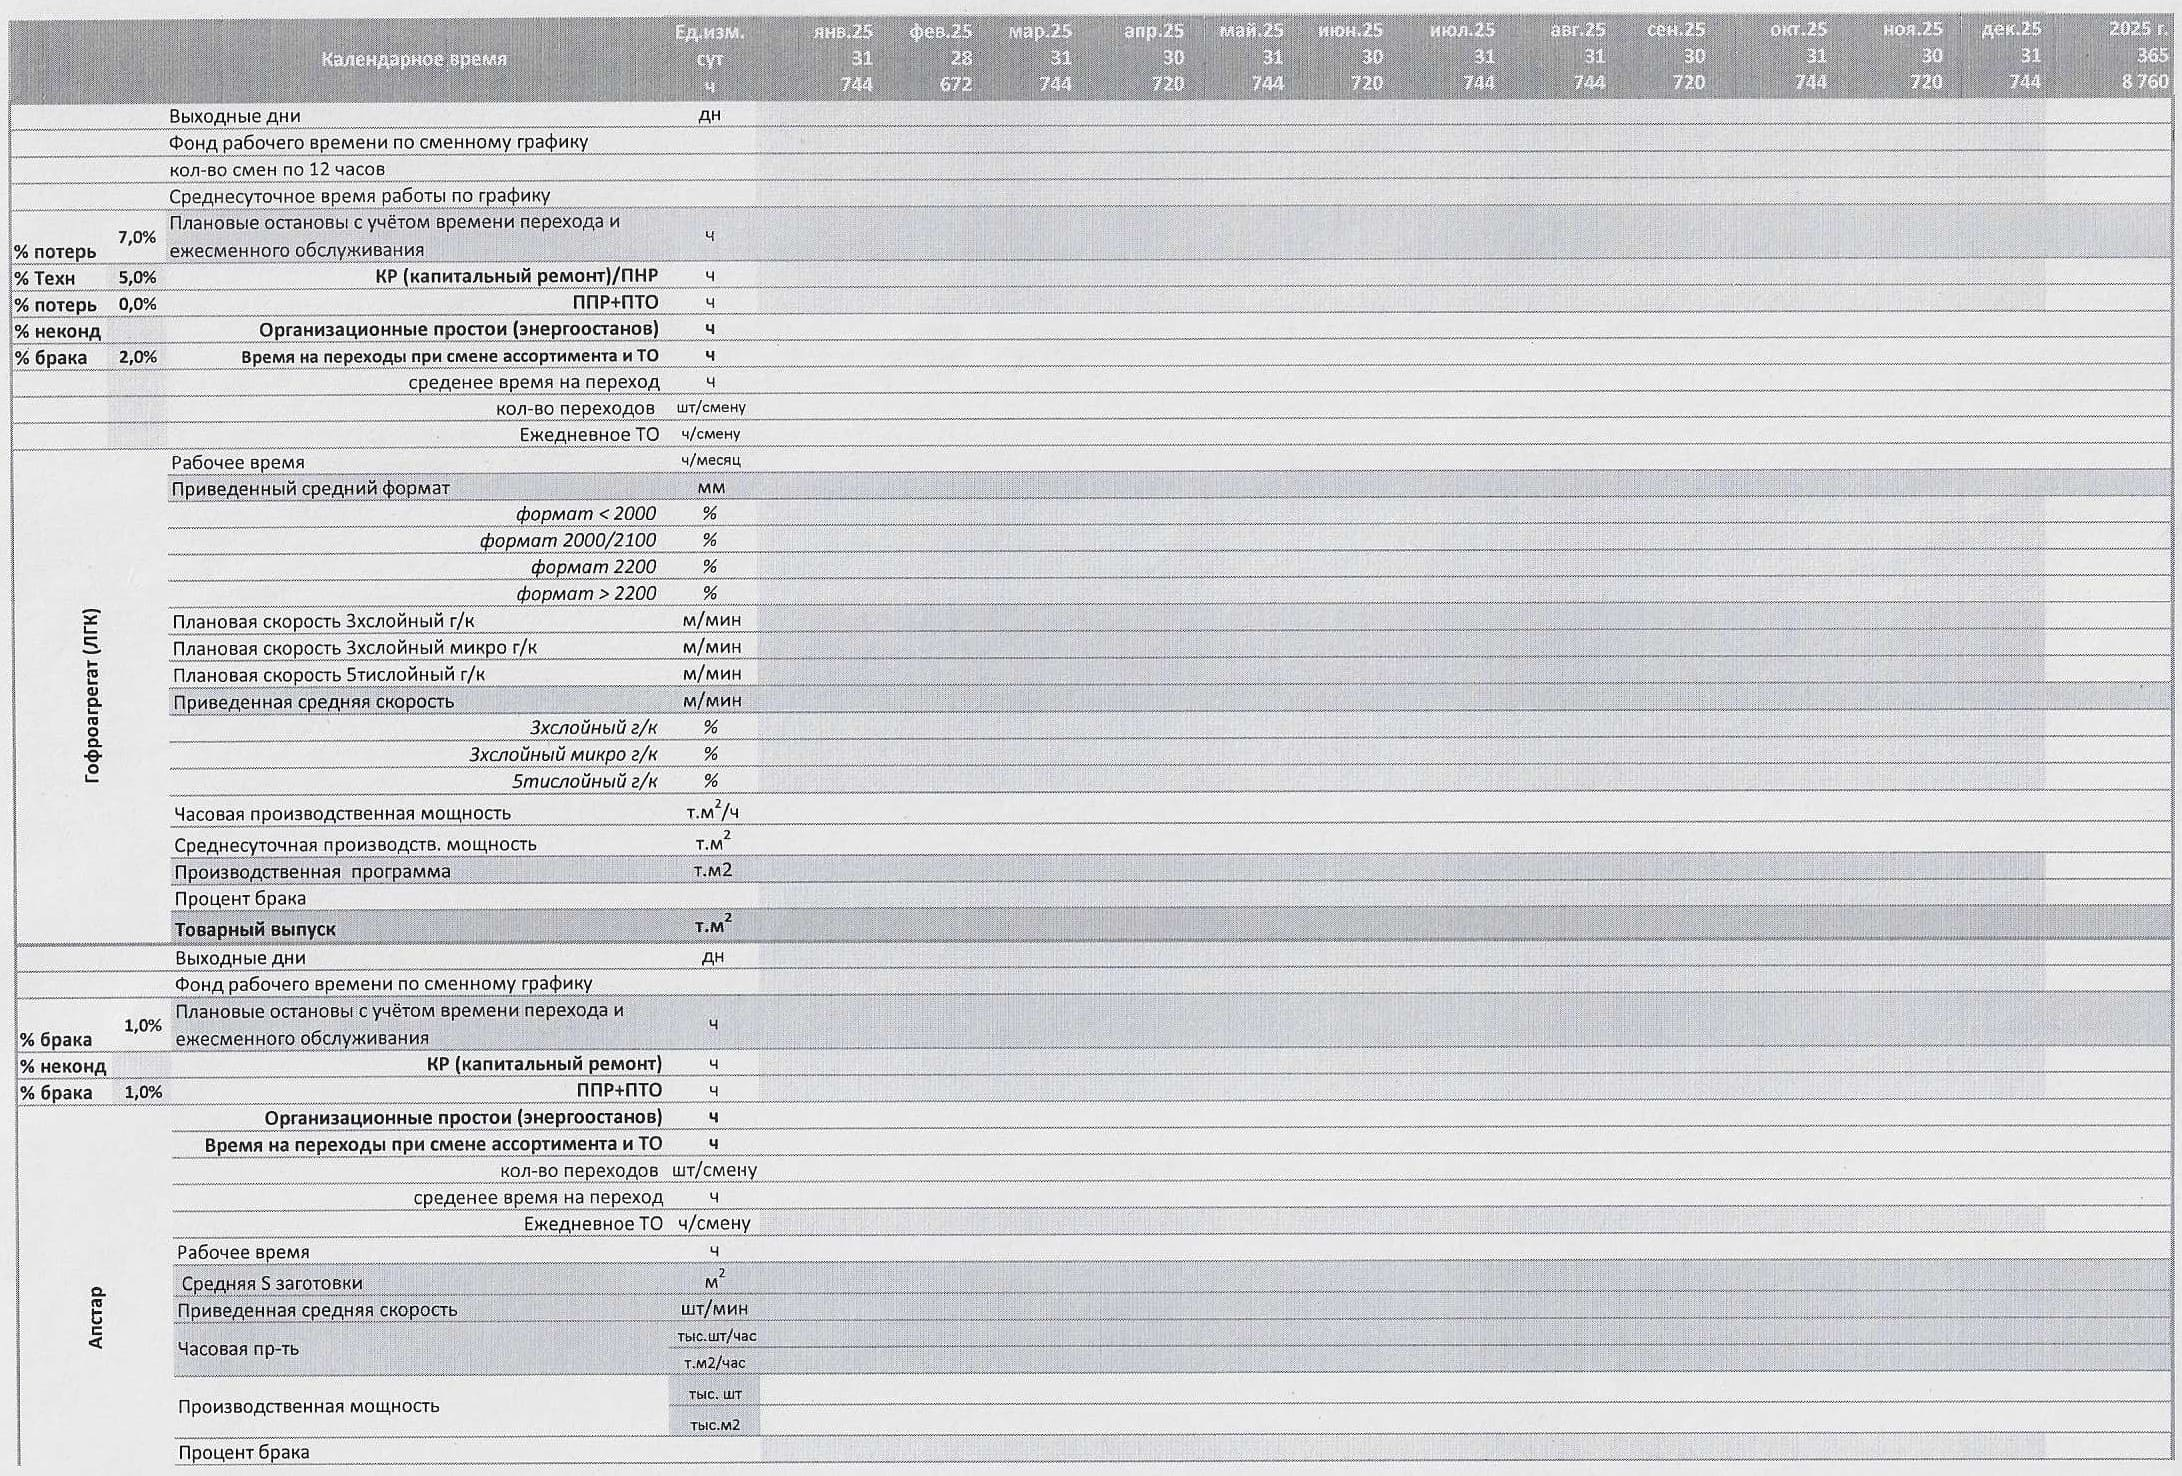
\includegraphics[height=0.6\textheight, width=1.3\textwidth, angle=90, keepaspectratio]{Pics/XI.1.jpg}
\end{center}
\caption{Форма ПРОФИНТЕХПЛАН}
\label{pic:XI.1}
\end{figure}
\clearpage

\begin{figure}
\begin{center}
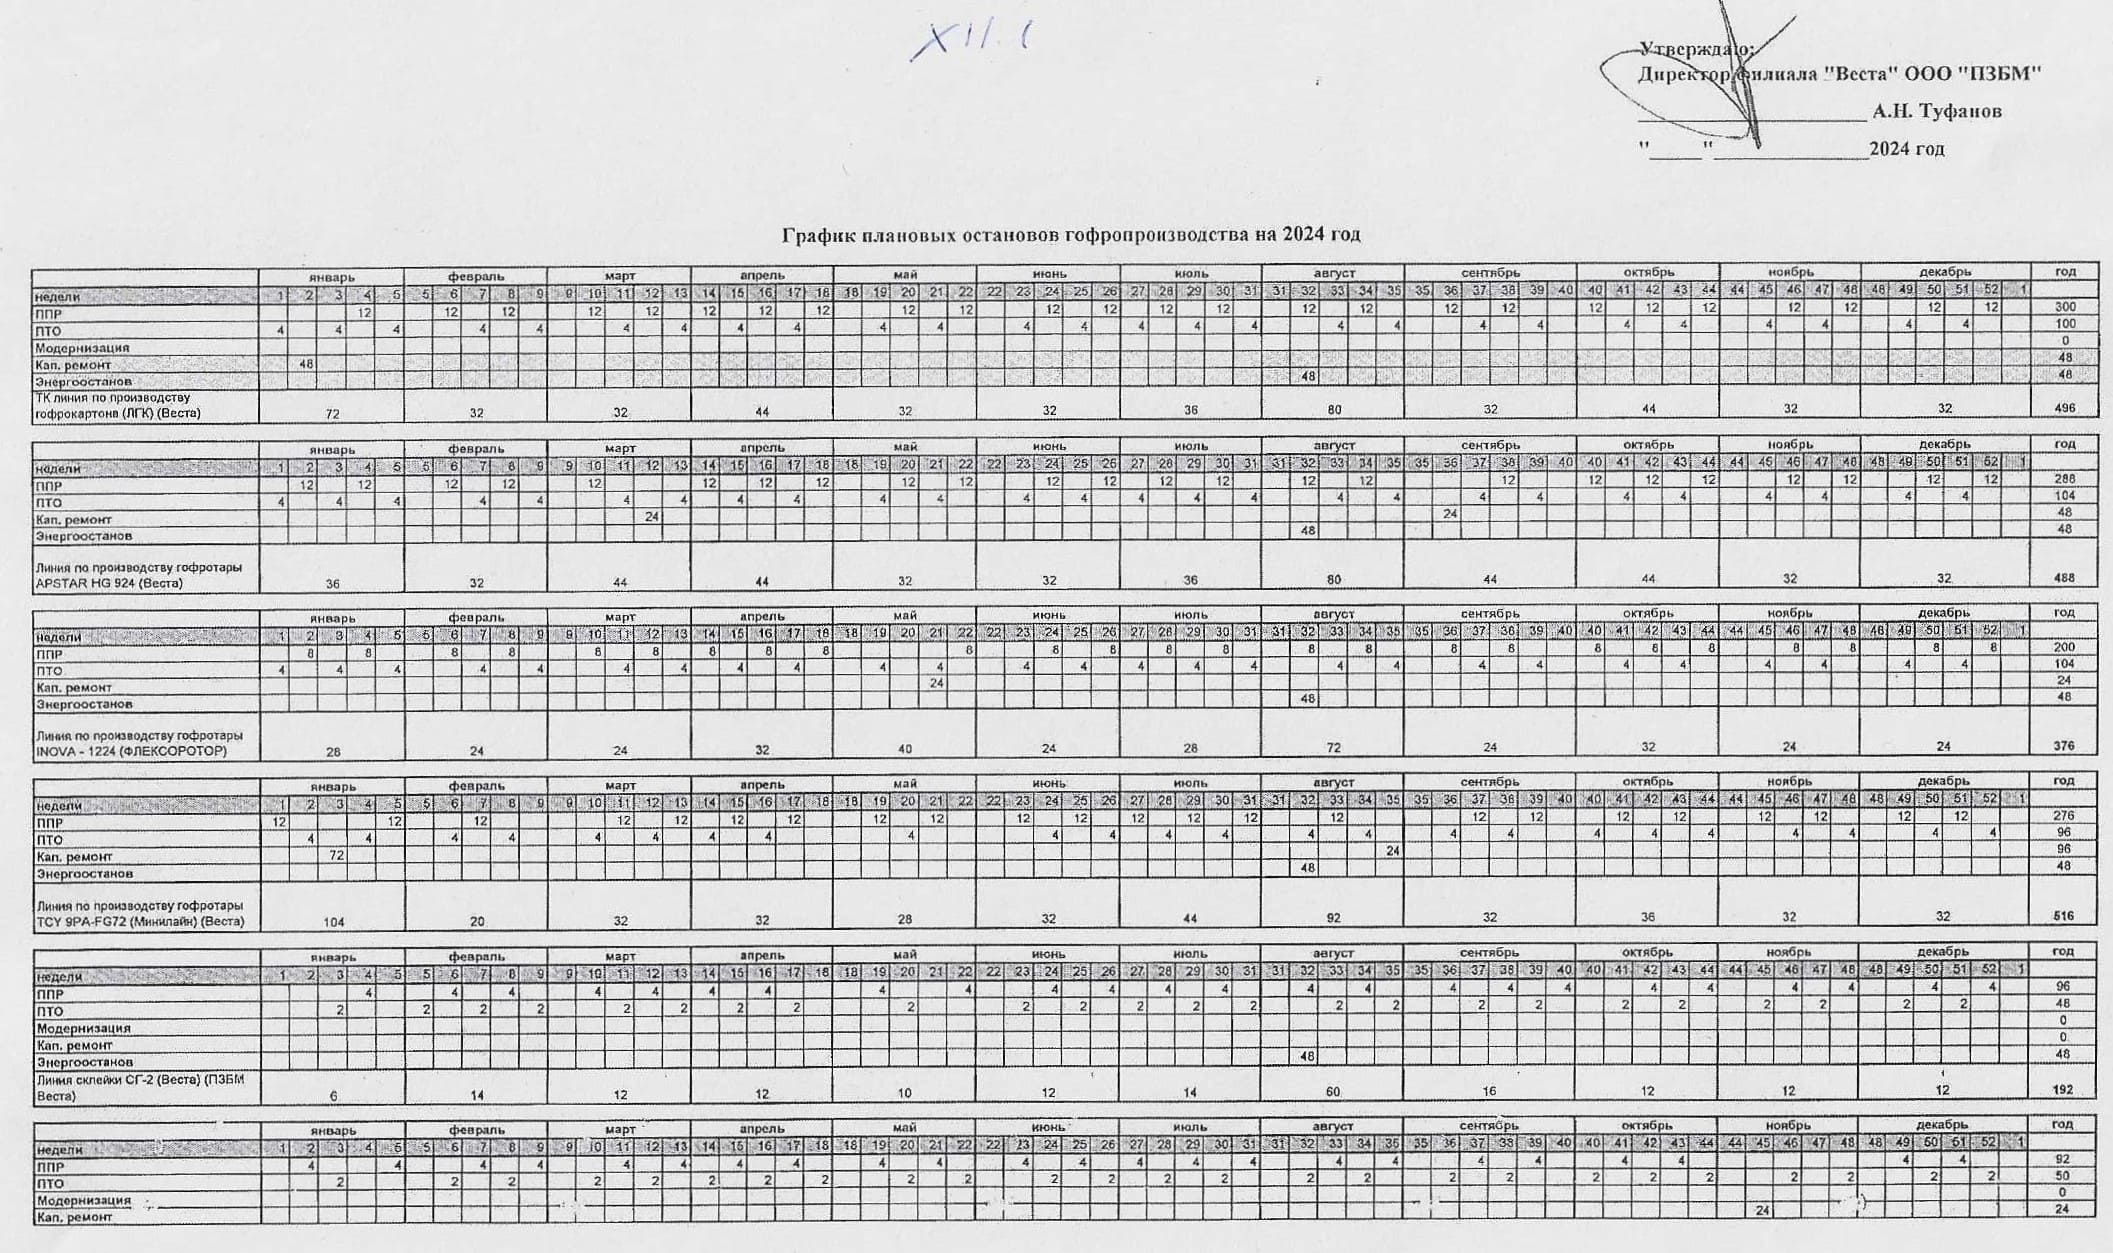
\includegraphics[height=0.6\textheight, width=1.3\textwidth, angle=90, keepaspectratio]{Pics/XII.1.jpg}
\end{center}
\caption{Годовой график плановых остановов}
\label{pic:XII.1.jpg}
\end{figure}
\clearpage

\begin{figure}
\begin{center}
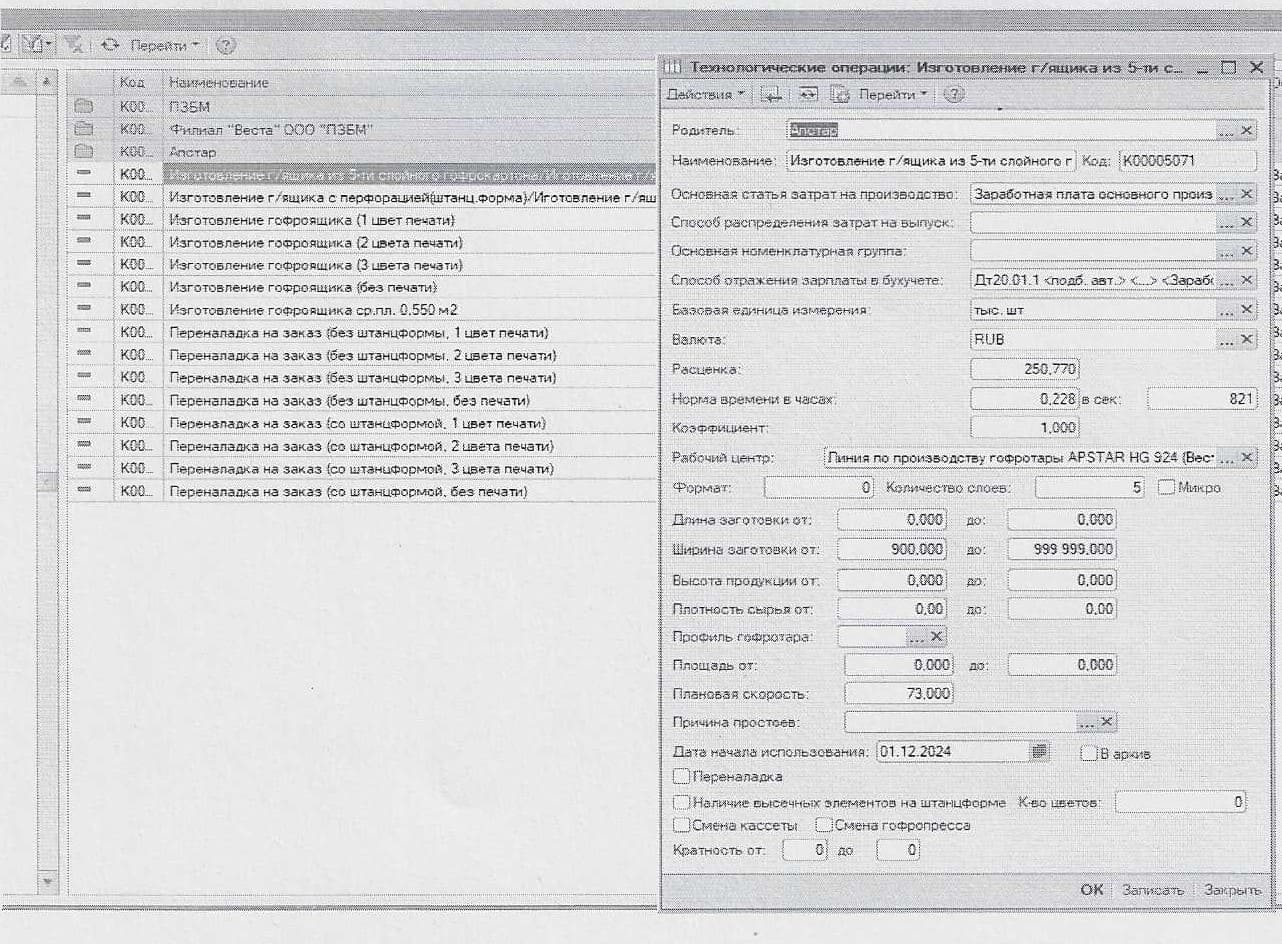
\includegraphics[height=0.6\textheight, width=1.3\textwidth, angle=90, keepaspectratio]{Pics/XI.12.jpg}
\end{center}
\caption{Нормирование времени и расценки в 1C:УПП}
\label{pic:XI.12.jpg}
\end{figure}
\clearpage

\begin{figure}
\begin{center}
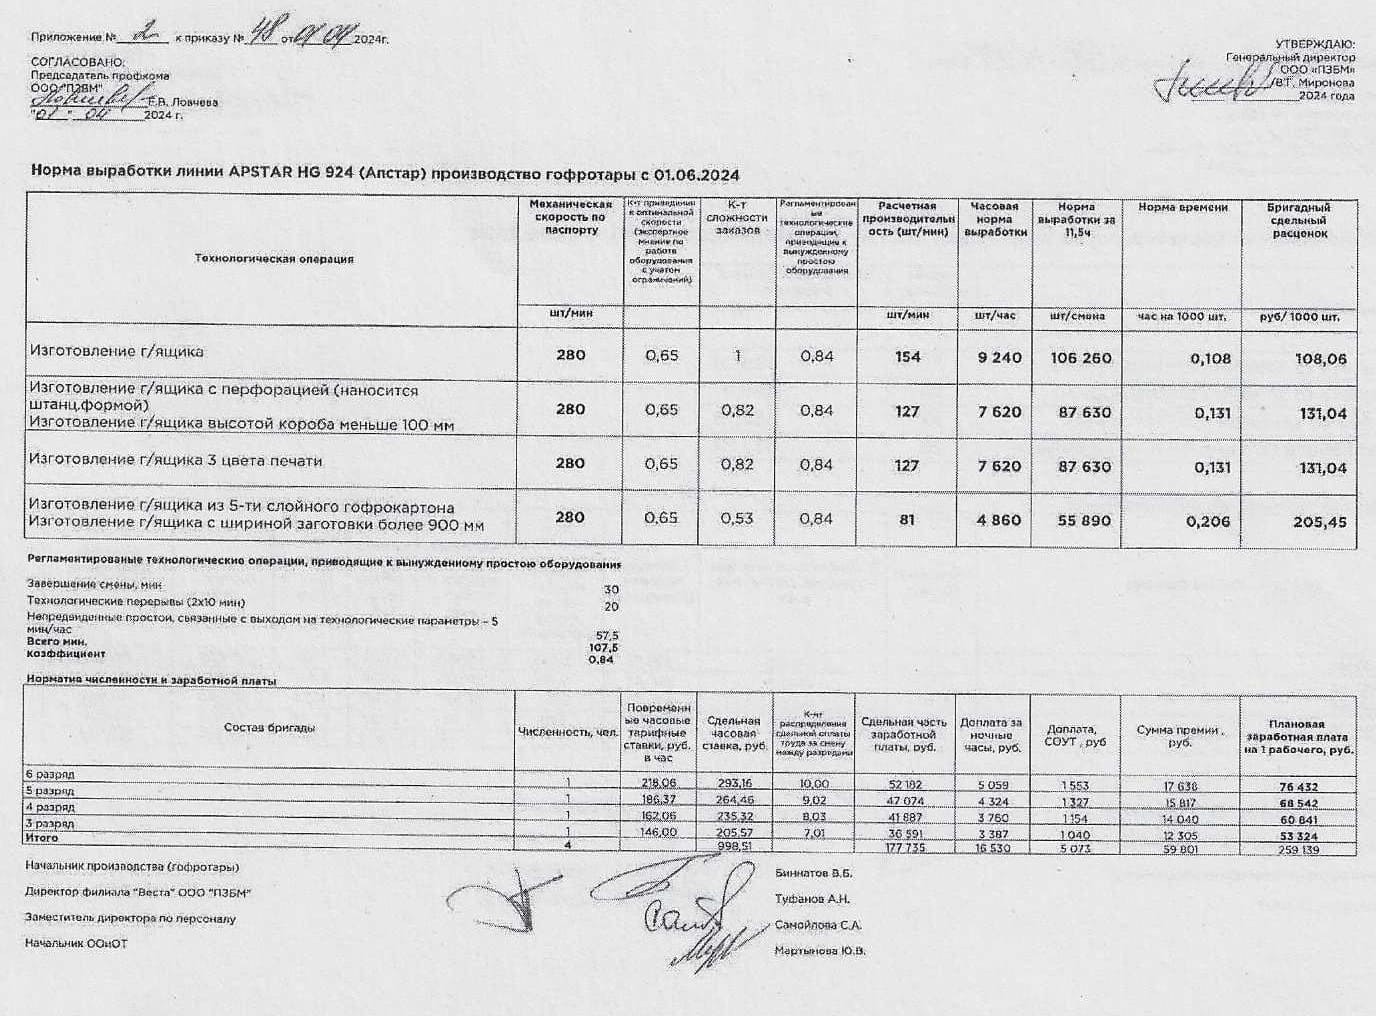
\includegraphics[height=0.6\textheight, width=1.3\textwidth, angle=90, keepaspectratio]{Pics/XI.11.jpg}
\end{center}
\caption{Утвержденная норма выработки на линию Апстар}
\label{pic:XI.11.jpg}
\end{figure}
\clearpage

\begin{figure}
\begin{center}
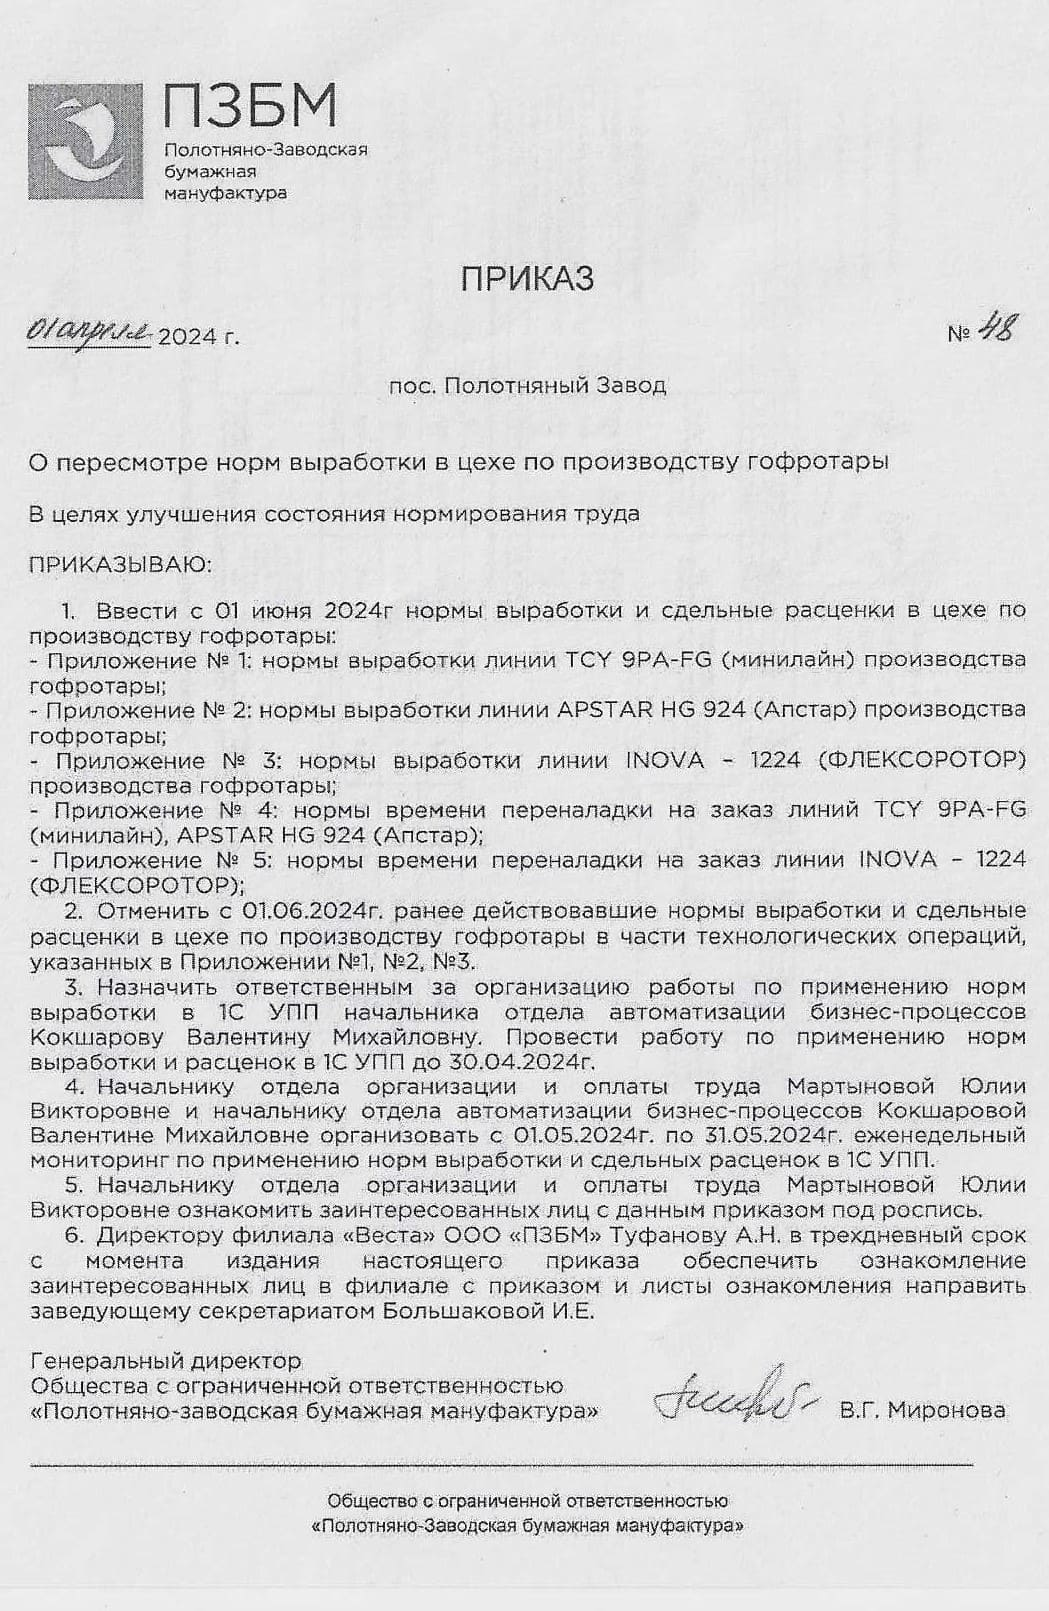
\includegraphics[height=0.8\textheight, width=1.5\textwidth, keepaspectratio]{Pics/XI.11..jpg}
\end{center}
\caption{Приказ о пересмотре норм выработки}
\label{pic:XI.11..jpg}
\end{figure}
\clearpage

\begin{figure}
\begin{center}
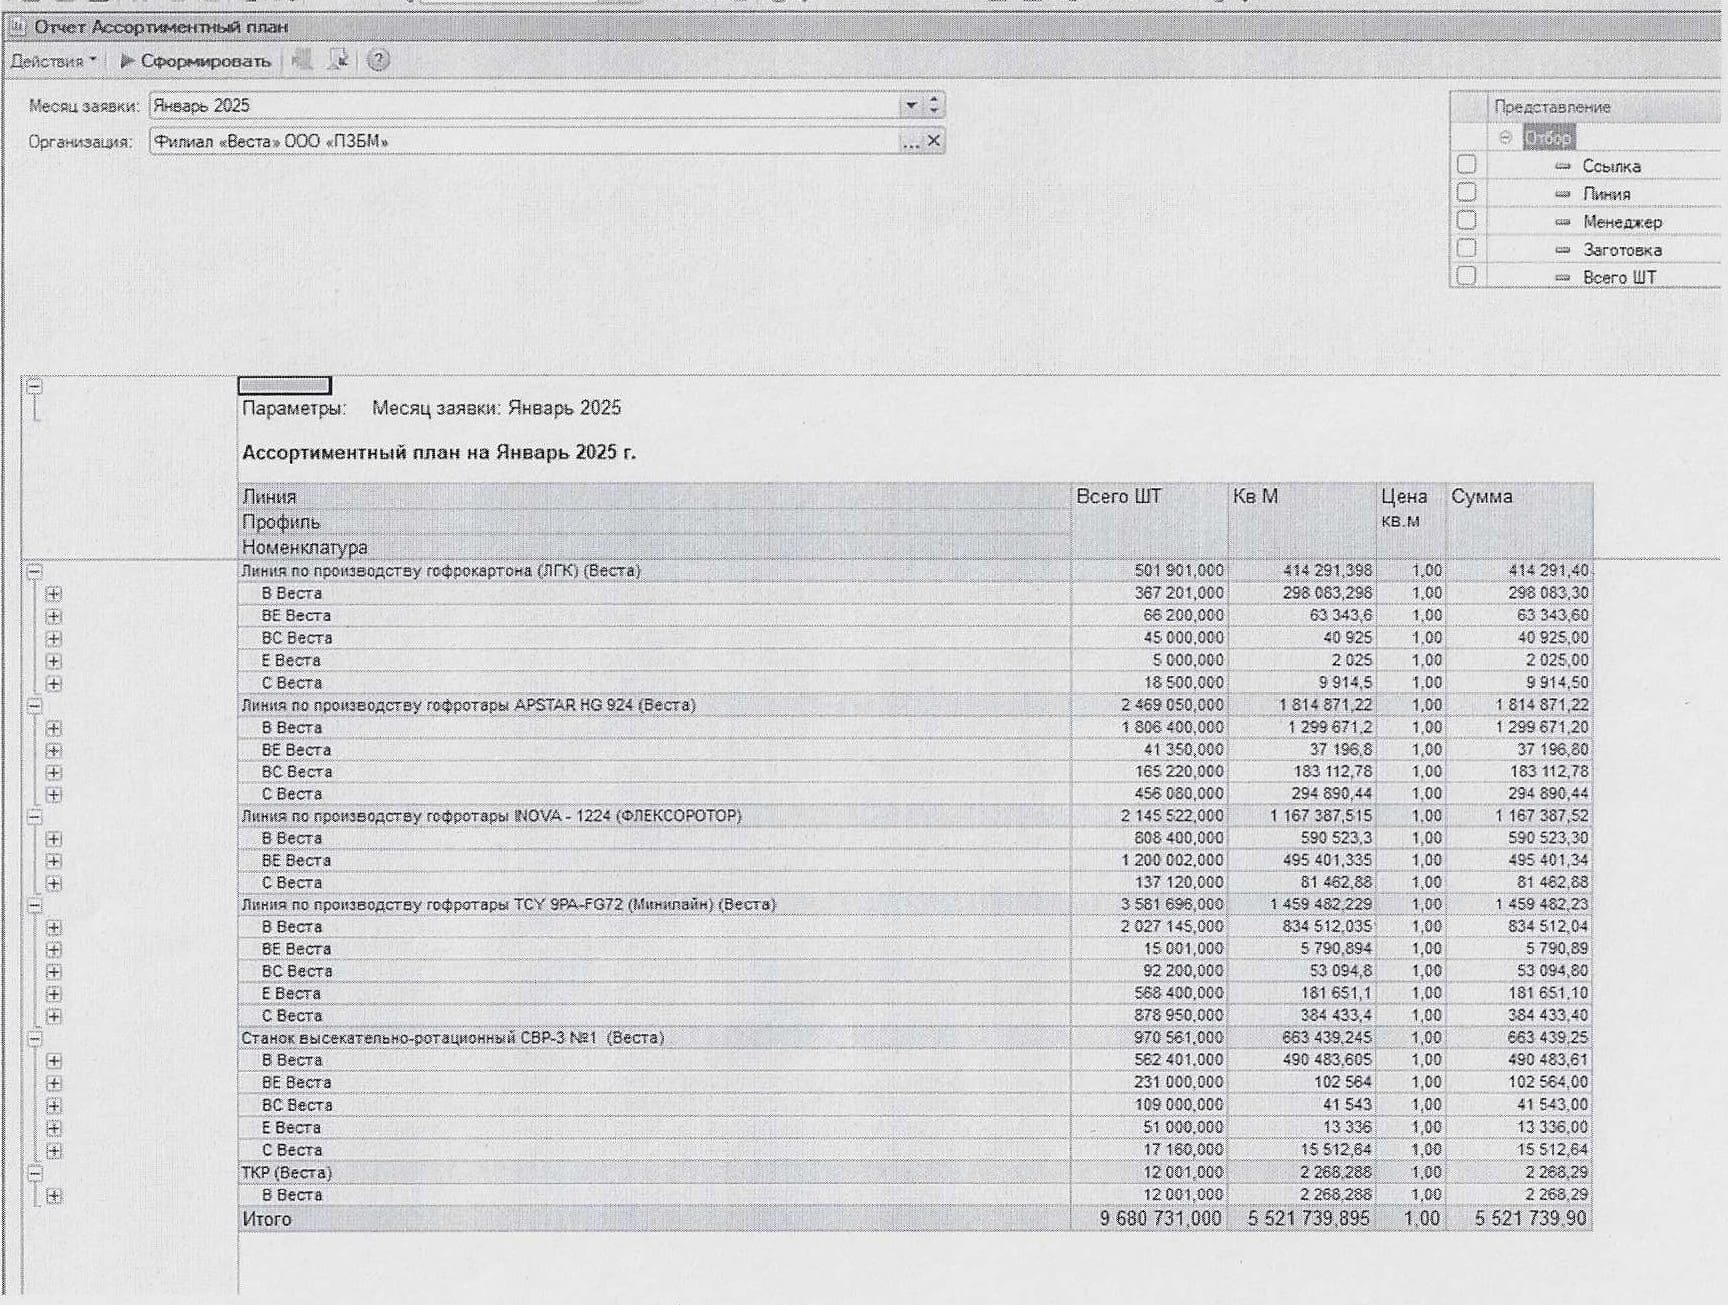
\includegraphics[height=0.5\textheight, width=1.3\textwidth, keepaspectratio]{Pics/I.5.6..jpg}
\end{center}
\caption{Форма Ассортиментный план}
\label{pic:I.5.6..jpg}
\end{figure}
\clearpage

\begin{figure}
\begin{center}
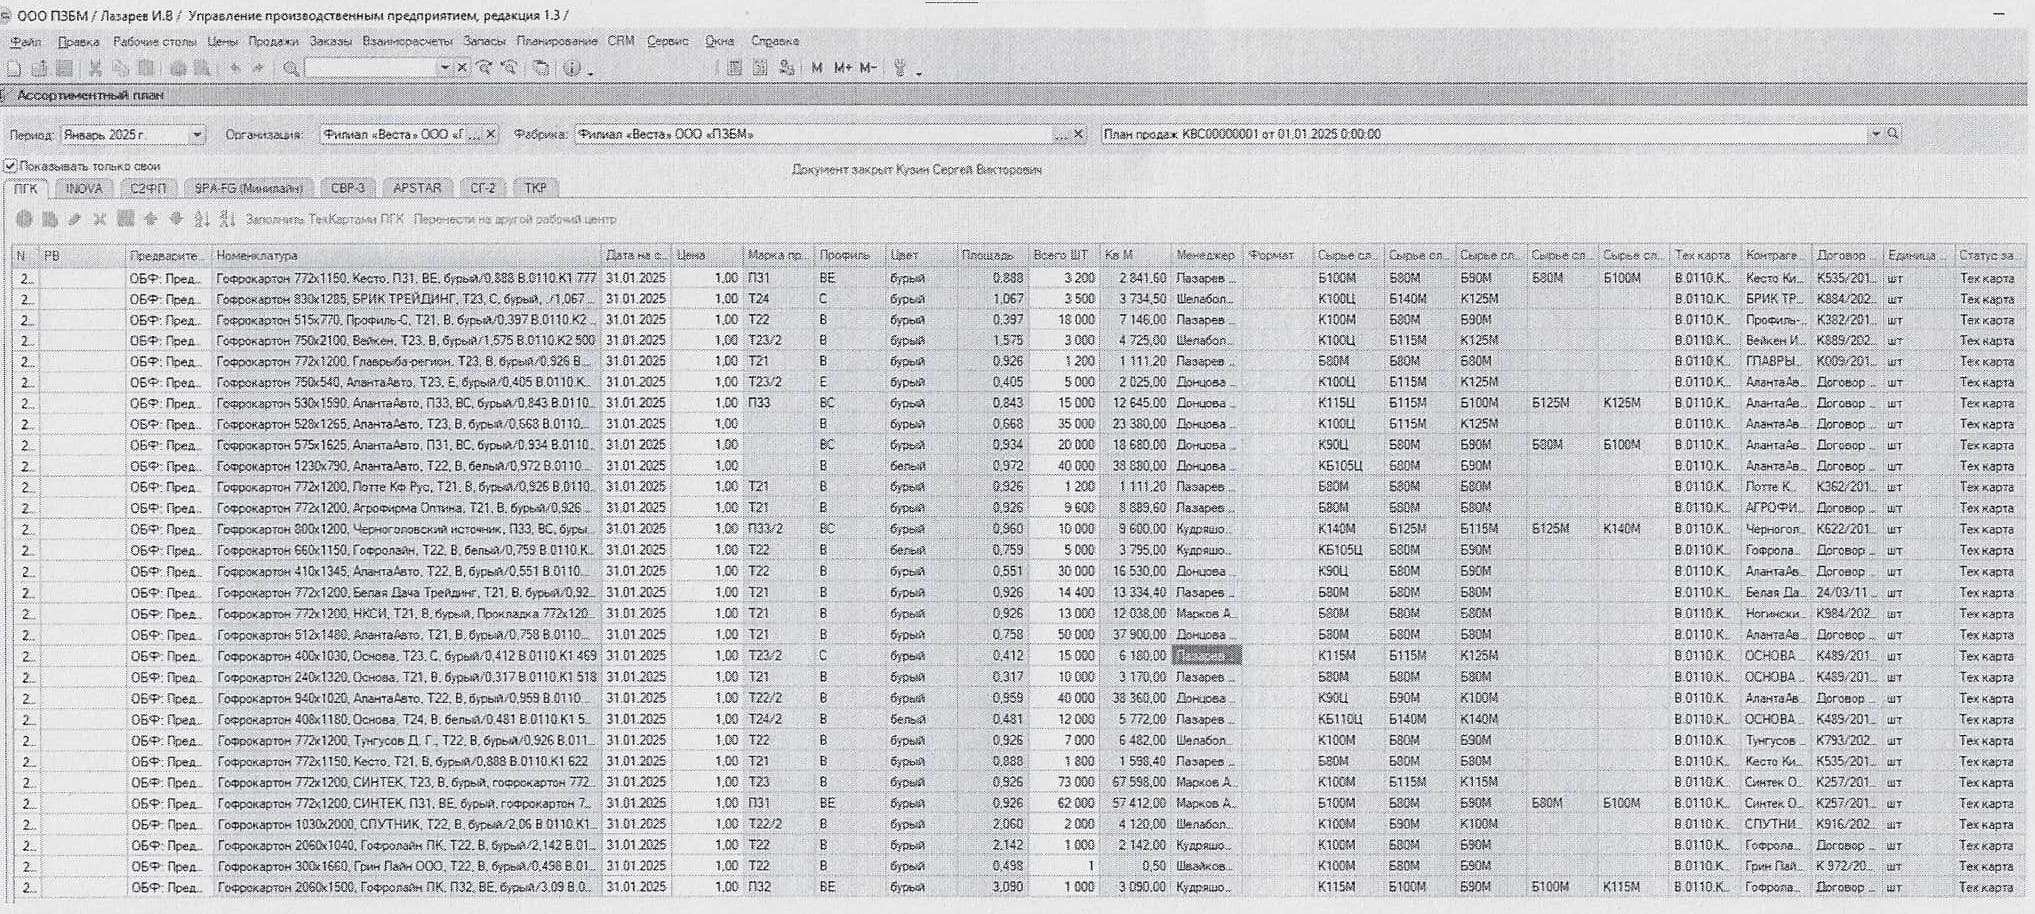
\includegraphics[height=0.3\textheight, width=1.3\textwidth, angle=90, keepaspectratio]{Pics/I.5.6.jpg}
\end{center}
\caption{Расширенная Форма Ассортиментный план}
\label{pic:I.5.6.jpg}
\end{figure}
\clearpage

%\ifx \notincludehead\undefined
\normalsize
\end{document}
\fi
\newpage
\subsection{Оперативное планирование продаж}
\label{bp:salesplan}


Оперативным планированием продаж на ПРЕДПРИЯТИИ занимаются менеджеры отдела продаж ООО ТД ''ФОРМАТ''. Все заказы/заявки оформляются ими в системе 1С: УПП (рис. \ref{pic:Рабочее место менеджера.jpg}).

Заявки/заказы от покупателей каждому менеджеру поступают по электронной почте, через мессенджеры. Форма подачи свободная (рис. \ref{pic:I.2.}).

После получения заявки менеджер в 1С: УПП производит следующие действия:
\begin{itemize}
    \item проверяет наличие ранее разработанных активных технологических карт по ГП через вкладку ''Технологические карты'' (рис. \ref{pic:II.4.jpg}); 
    \item проверяет, через отчет ''Загрузка оборудования по предварительным заявкам'' (рис. \ref{pic:I.5.2...jpg}) возможность размещения заказа на производство на ту или иную линию на желаемую дату;
    \item создает документ ''Предварительная заявка'' (рис. \ref{pic:I.5.jpg}) на резервирование времени работы требуемого для изготовления заказа оборудования;
    \item в табличной части указывает номенклатуру ГП, необходимое количество и дату реализации ГП;
    \item после проведения документа автоматически создается ''Заказ на производство'' (рис. \ref{pic:I.5.4.jpg}), в котором дата отгрузки (информация для производства) будет смещена на один день раньше, установленной менеджером;
    \item на основании документа ''Заказ покупателя''
    % \footnote[1]{''Заказ покупателя'' - необходим для формирования заявки на отгрузку, и создания документов ''План отгрузок'' и ''План реализации''.} 
    создает документ ''Заявку на отгрузку'' (рис. \ref{pic:I.5.5.jpg}), в котором указывает дату отгрузки, адрес доставки, номенклатуру ГП, цену реализации, количество единиц ГП. 
    Документ ''Заказ покупателя'' необходим для формирования заявки на отгрузку и создания документов ''План отгрузок'' и ''План реализации''.
   
\end{itemize}


Каждый менеджер после оформления предварительной заявки и создания заказа на производство, сообщает об этом в отдел планирования по электронной почте. %(рис. \ref{pic:VII 1.jpg}). 


 
%При появлении от клиентов заявок от покупателей менеджеры регистрируют в системе СБИС документ ''Заявка покупателя'' (рис. \ref{pic:dd9}). Менеджеры формируют при необходимости счет на оплату из формы документа \ref{pic:dd8} или создают документ «Счет». 

%В системе СБИС менеджеры регистрируют все заявки покупателя.

%Выделено несколько крупных покупателей, по которым до 25 числа каждого месяца требуется создавать заявки покупателей в 1С: УПП. Таких клиентов только 50\%. 
%Составление списка заявок покупателей в системе СБИС 
% на начало месяца 
% можно условно назвать 
% является 
%оперативным планирование продаж.
%
%

\begin{figure}
\begin{center}
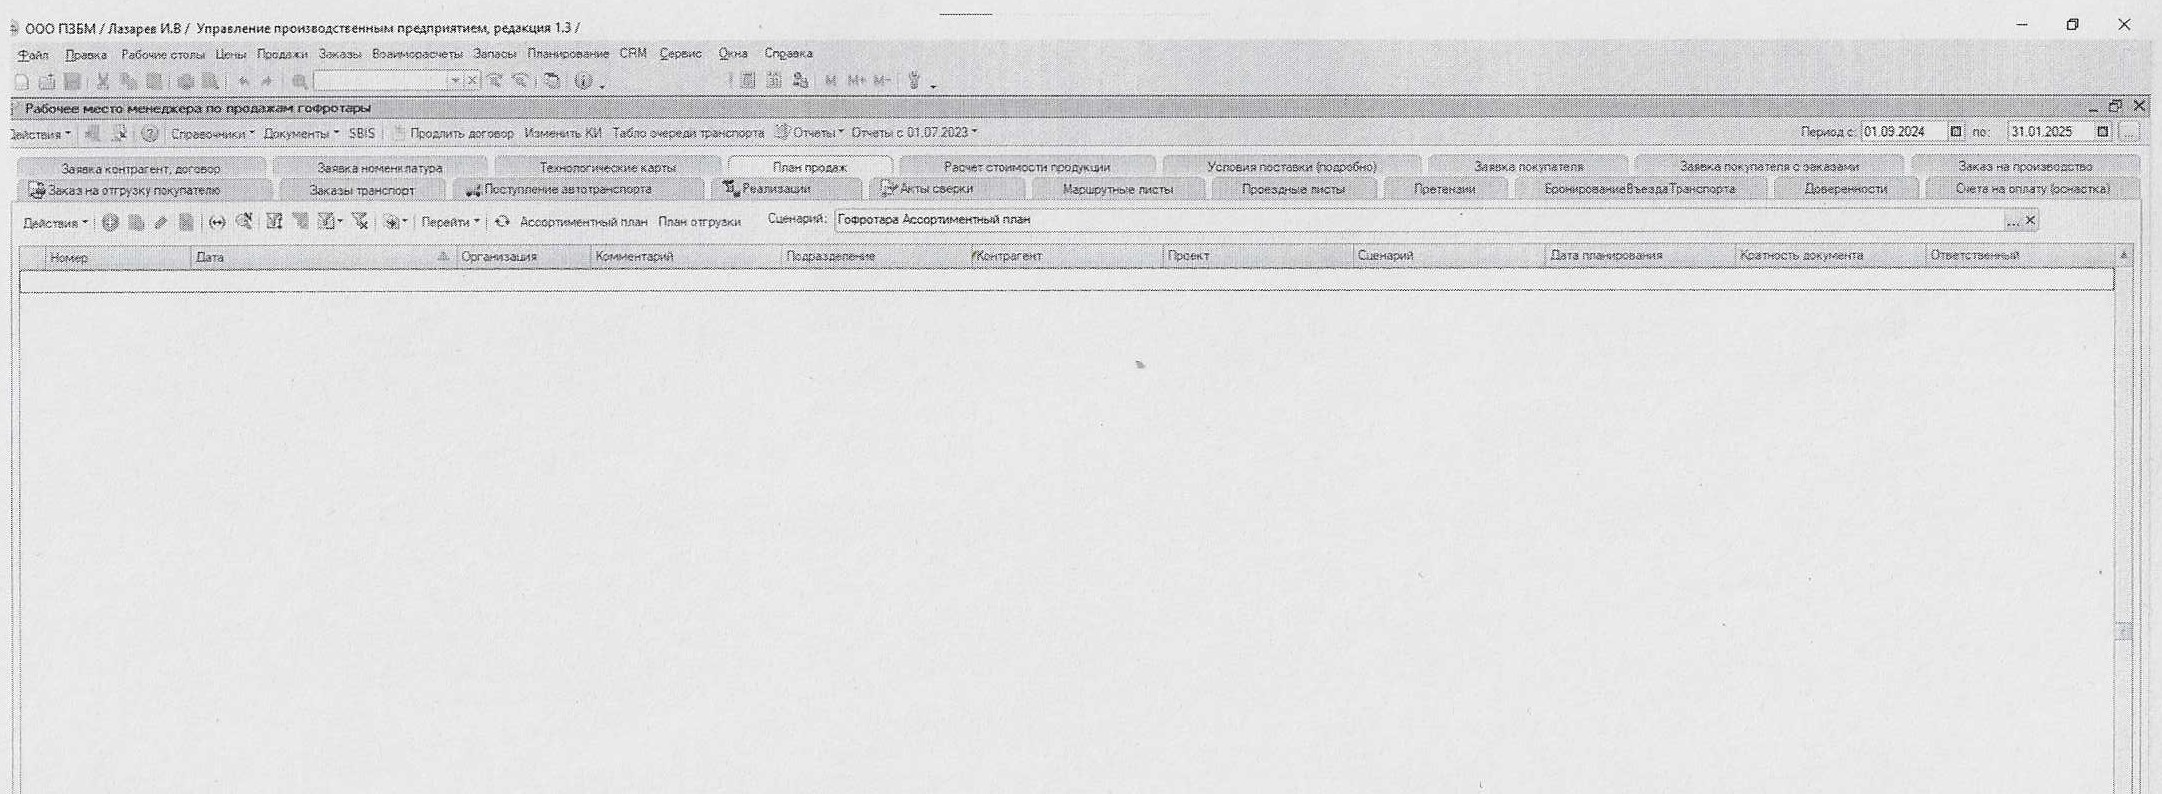
\includegraphics[height=0.25\textheight, angle=90, keepaspectratio]{Pics/Рабочее место менеджера.jpg}
\end{center}
\caption{Рабочий стол менеджера отдела продаж в 1С: УПП}
\label{pic:Рабочее место менеджера.jpg}
\end{figure}
\clearpage

%
\begin{figure}
\begin{center}
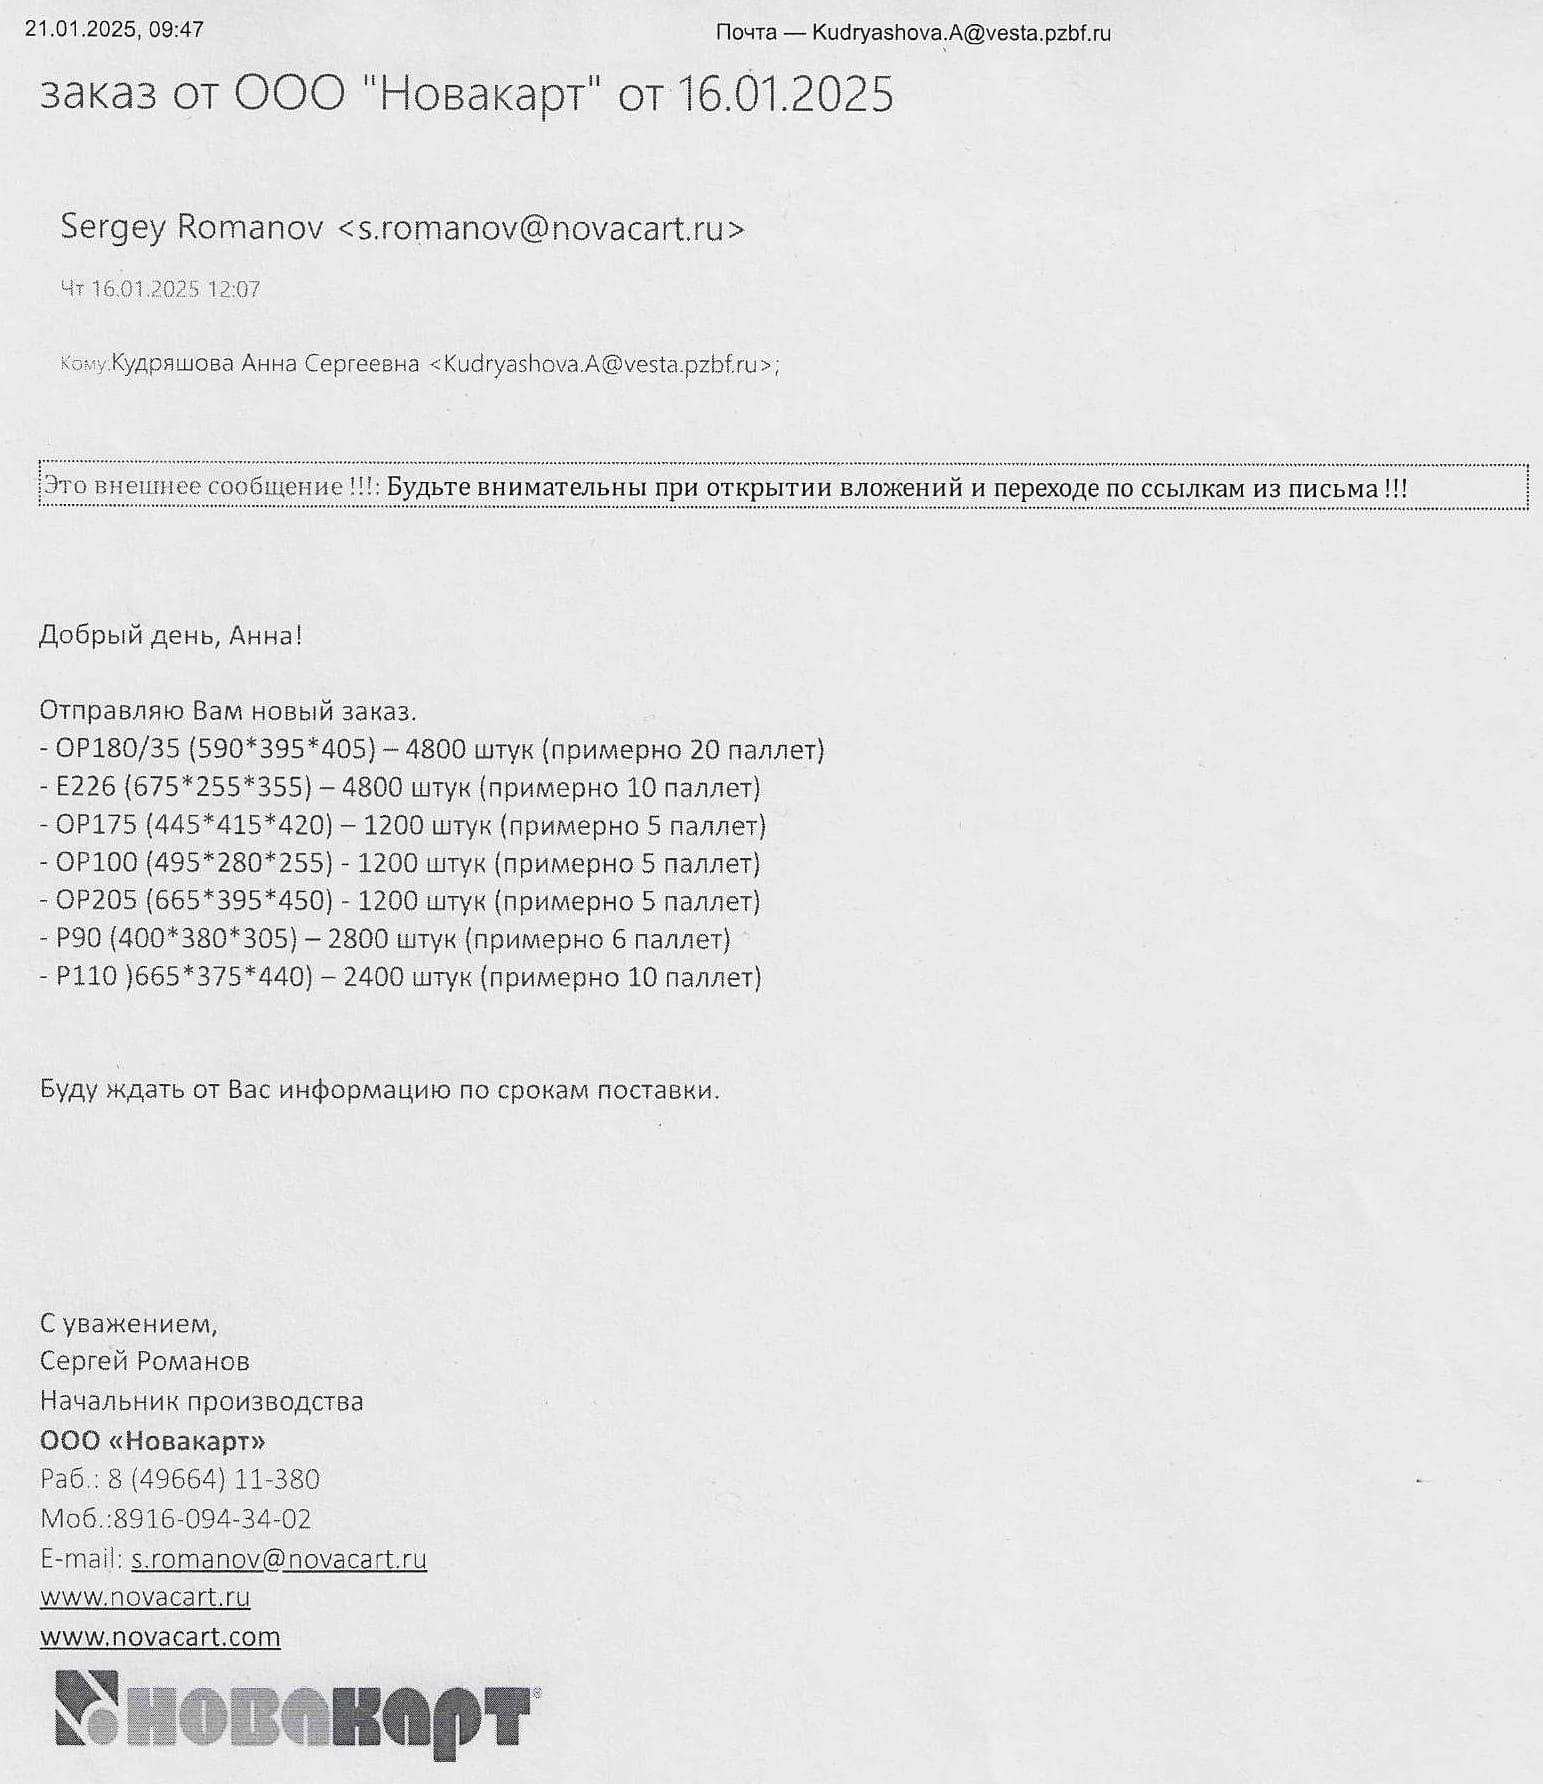
\includegraphics[height=0.7\textheight, keepaspectratio]{Pics/I.2..jpg}
\end{center}
\caption{Вид заявки от покупателя}
\label{pic:I.2.}
\end{figure}
\clearpage


\begin{figure}
\begin{center}
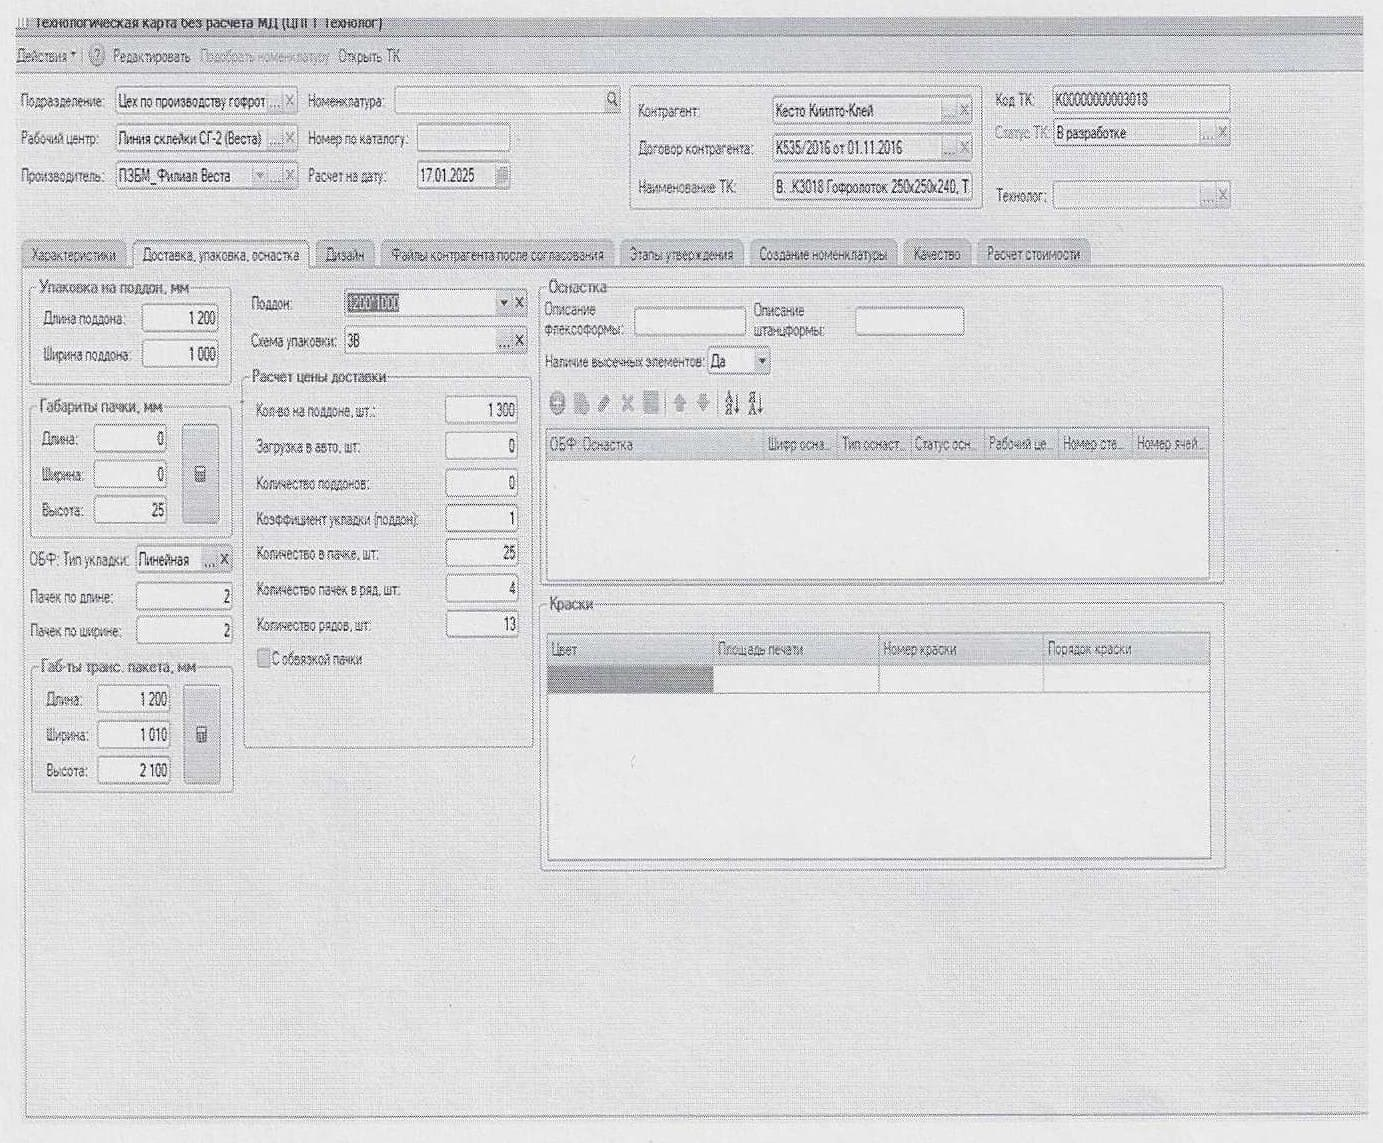
\includegraphics[height=0.5\textheight,  keepaspectratio]{Pics/II.4.jpg}
\end{center}
\caption{Форма Технологическая карта}
\label{pic:II.4.jpg}
\end{figure}
\clearpage



\begin{figure}
\begin{center}
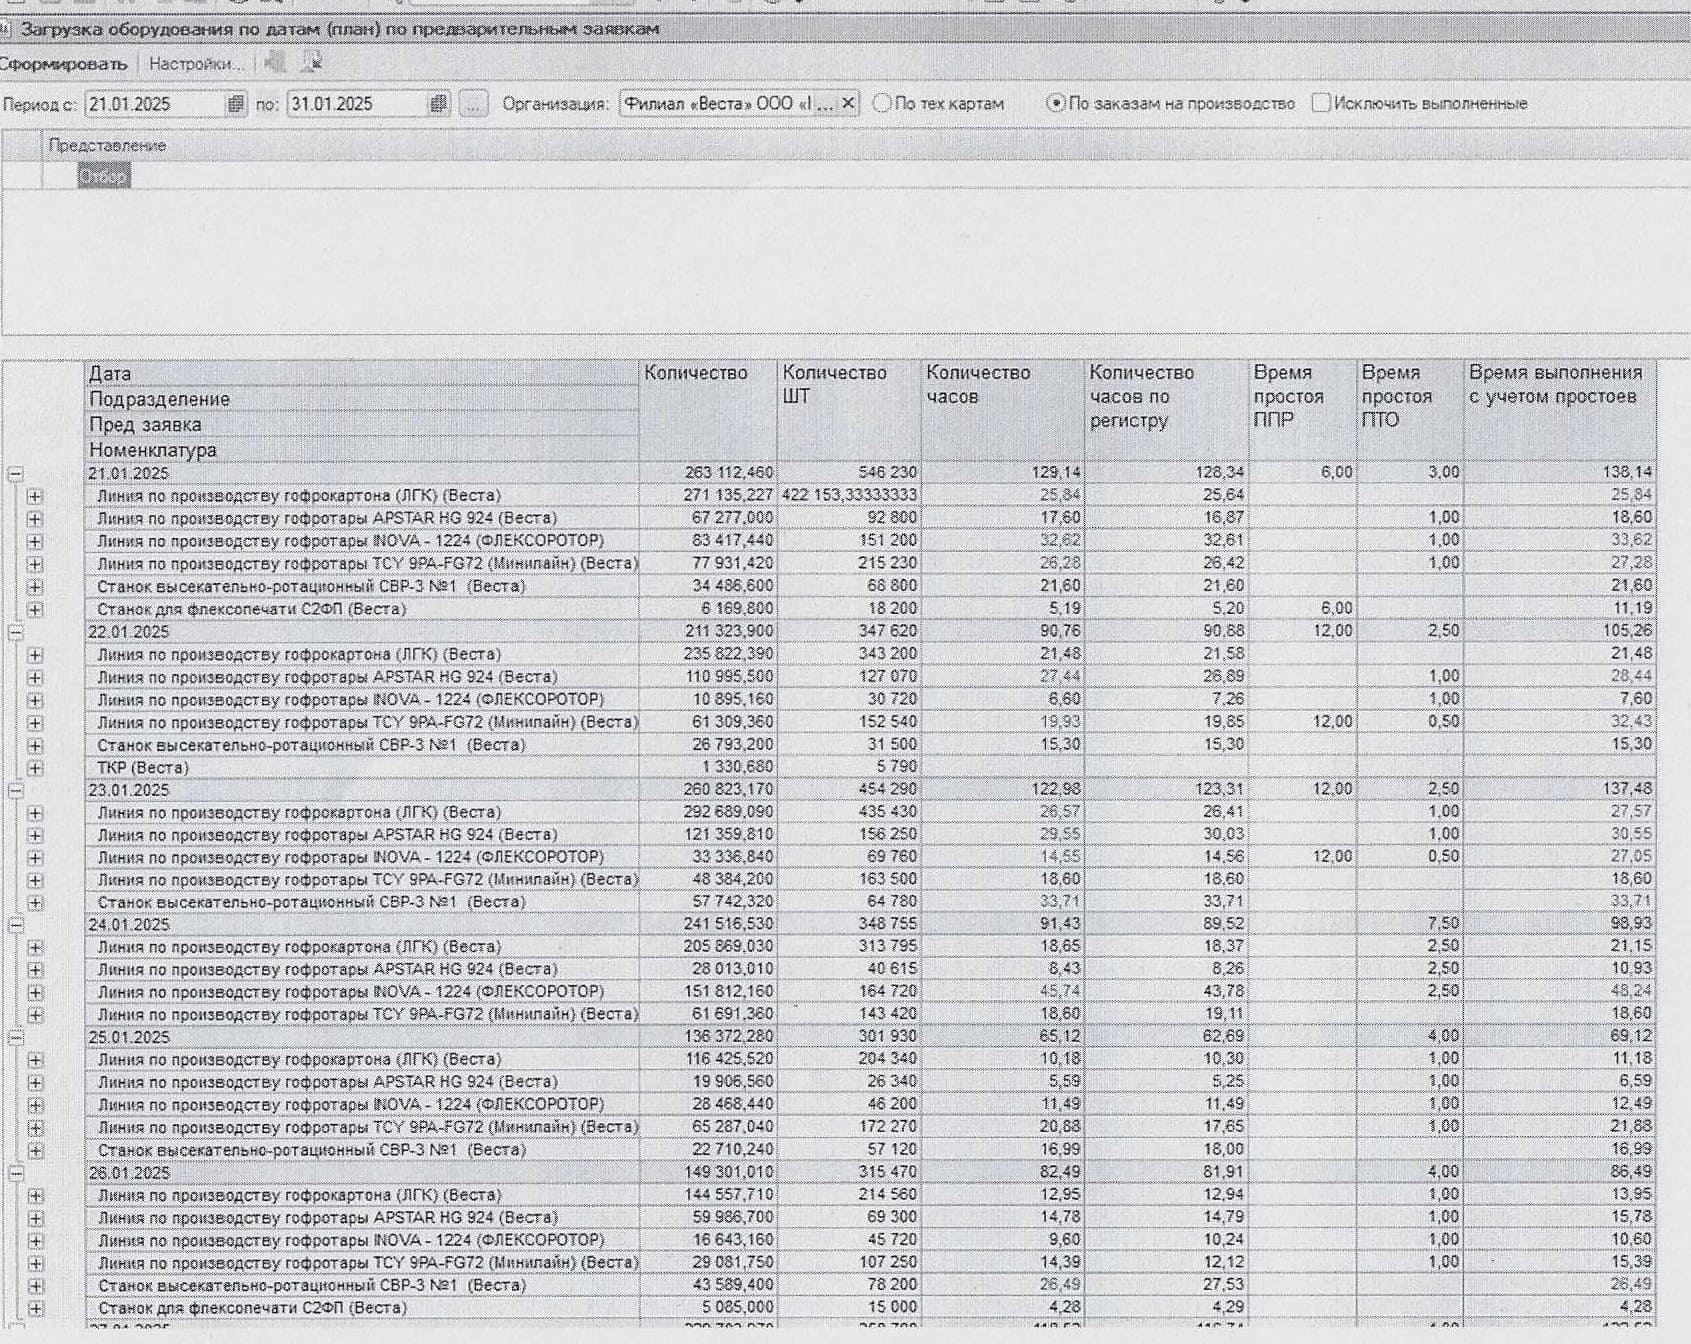
\includegraphics[height=0.5\textheight, keepaspectratio]{Pics/I.5.2...jpg}
\end{center}
\caption{Форма отчета Загрузка оборудования по предварительным заявкам}
\label{pic:I.5.2...jpg}
\end{figure}
%\clearpage



\begin{figure}
\begin{center}
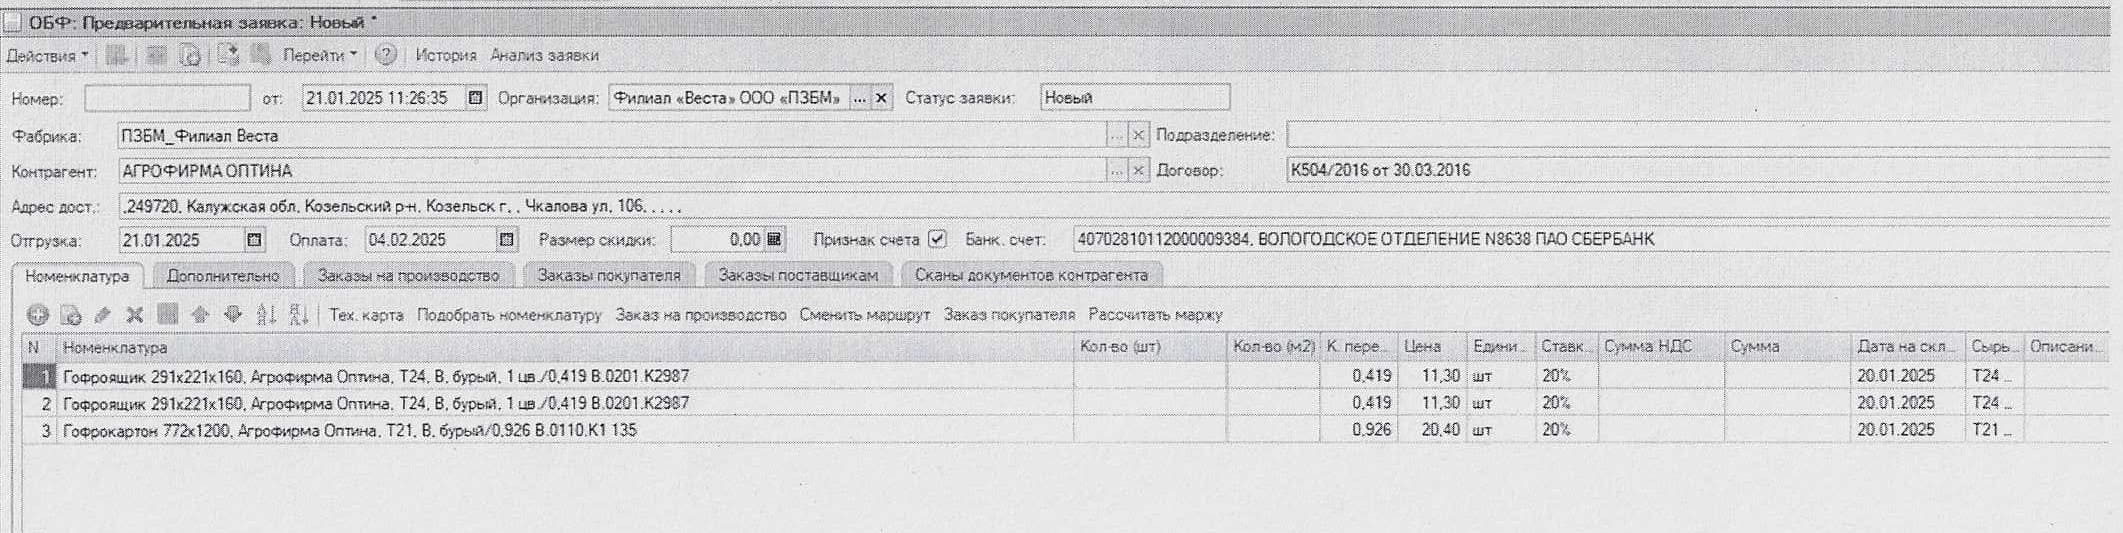
\includegraphics[height=0.15\textheight,  keepaspectratio]{Pics/I.5.jpg}
\end{center}
\caption{Форма создания предварительной заявки}
\label{pic:I.5.jpg}
\end{figure}
\clearpage

\begin{figure}
\begin{center}
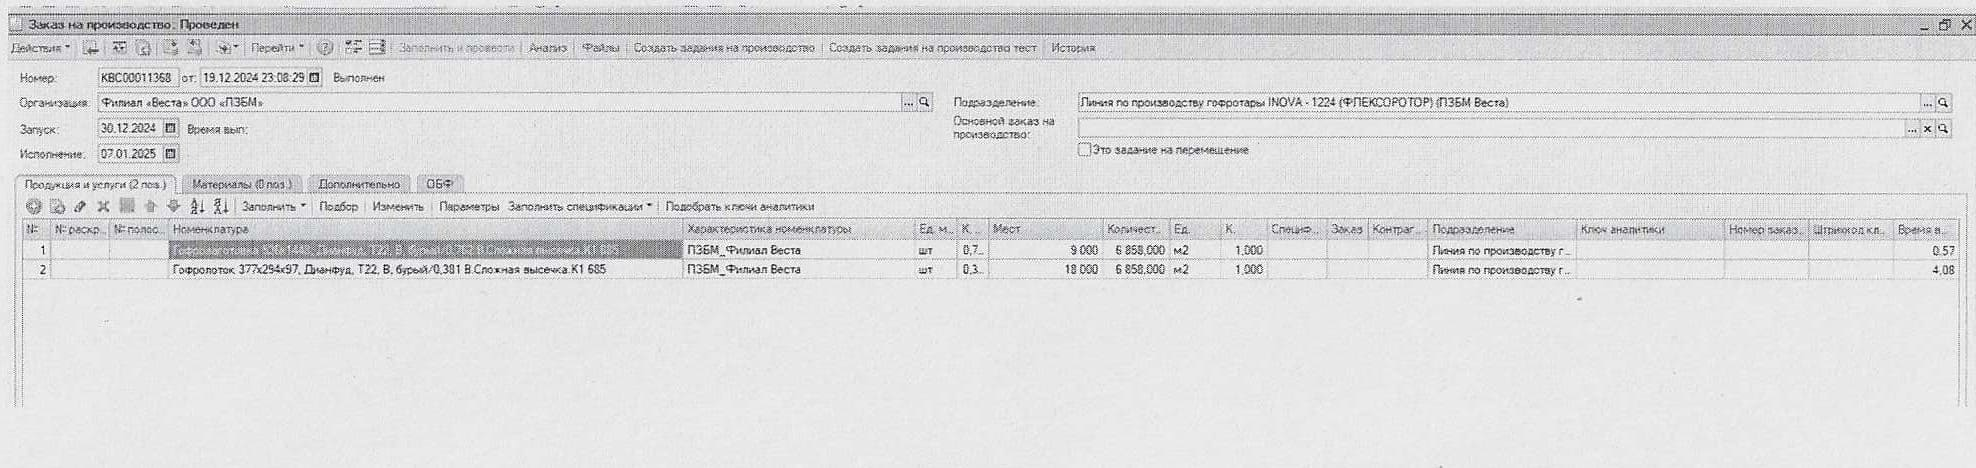
\includegraphics[height=0.15\textheight,  keepaspectratio]{Pics/I.5.4.jpg}
\end{center}
\caption{Форма заказ на производство}
\label{pic:I.5.4.jpg}
\end{figure}
%\clearpage

\begin{figure}
\begin{center}
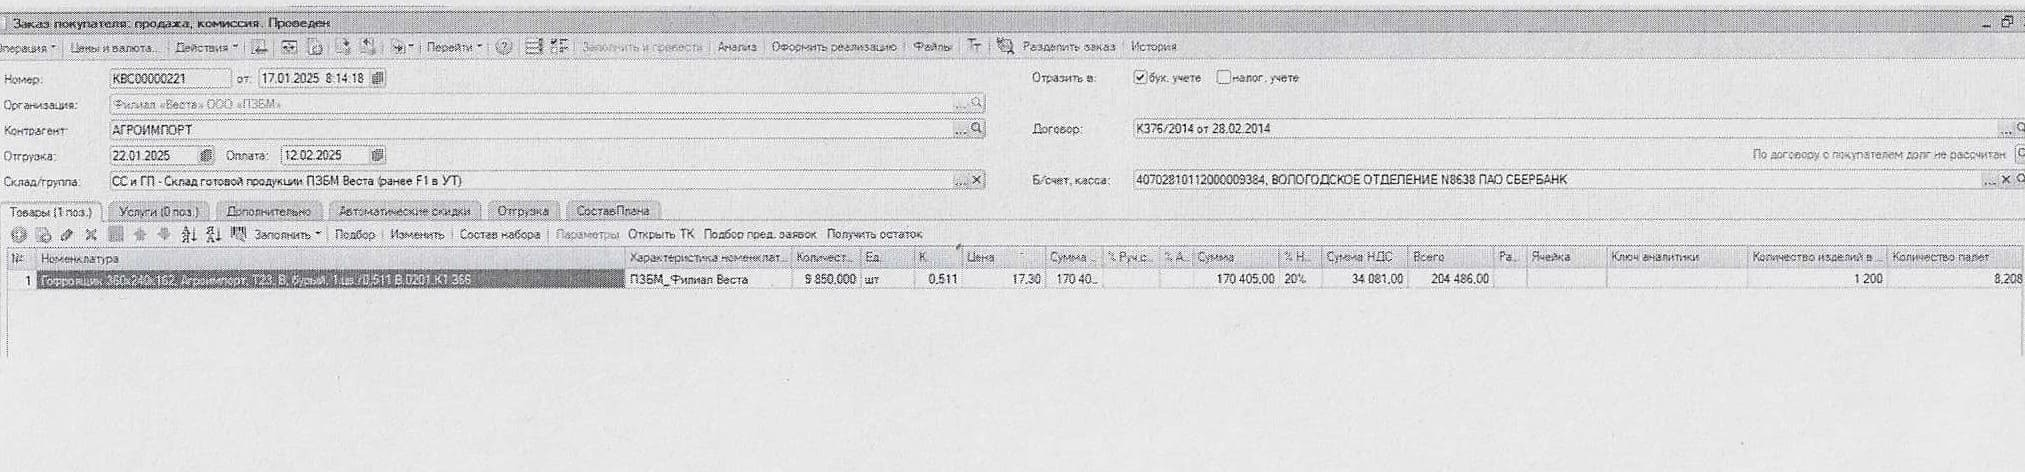
\includegraphics[height=0.15\textheight, keepaspectratio]{Pics/I.5.5.jpg}
\end{center}
\caption{Форма заявка покупателя}
\label{pic:I.5.5.jpg}
\end{figure}
\clearpage

%\begin{figure}
%\begin{center}
%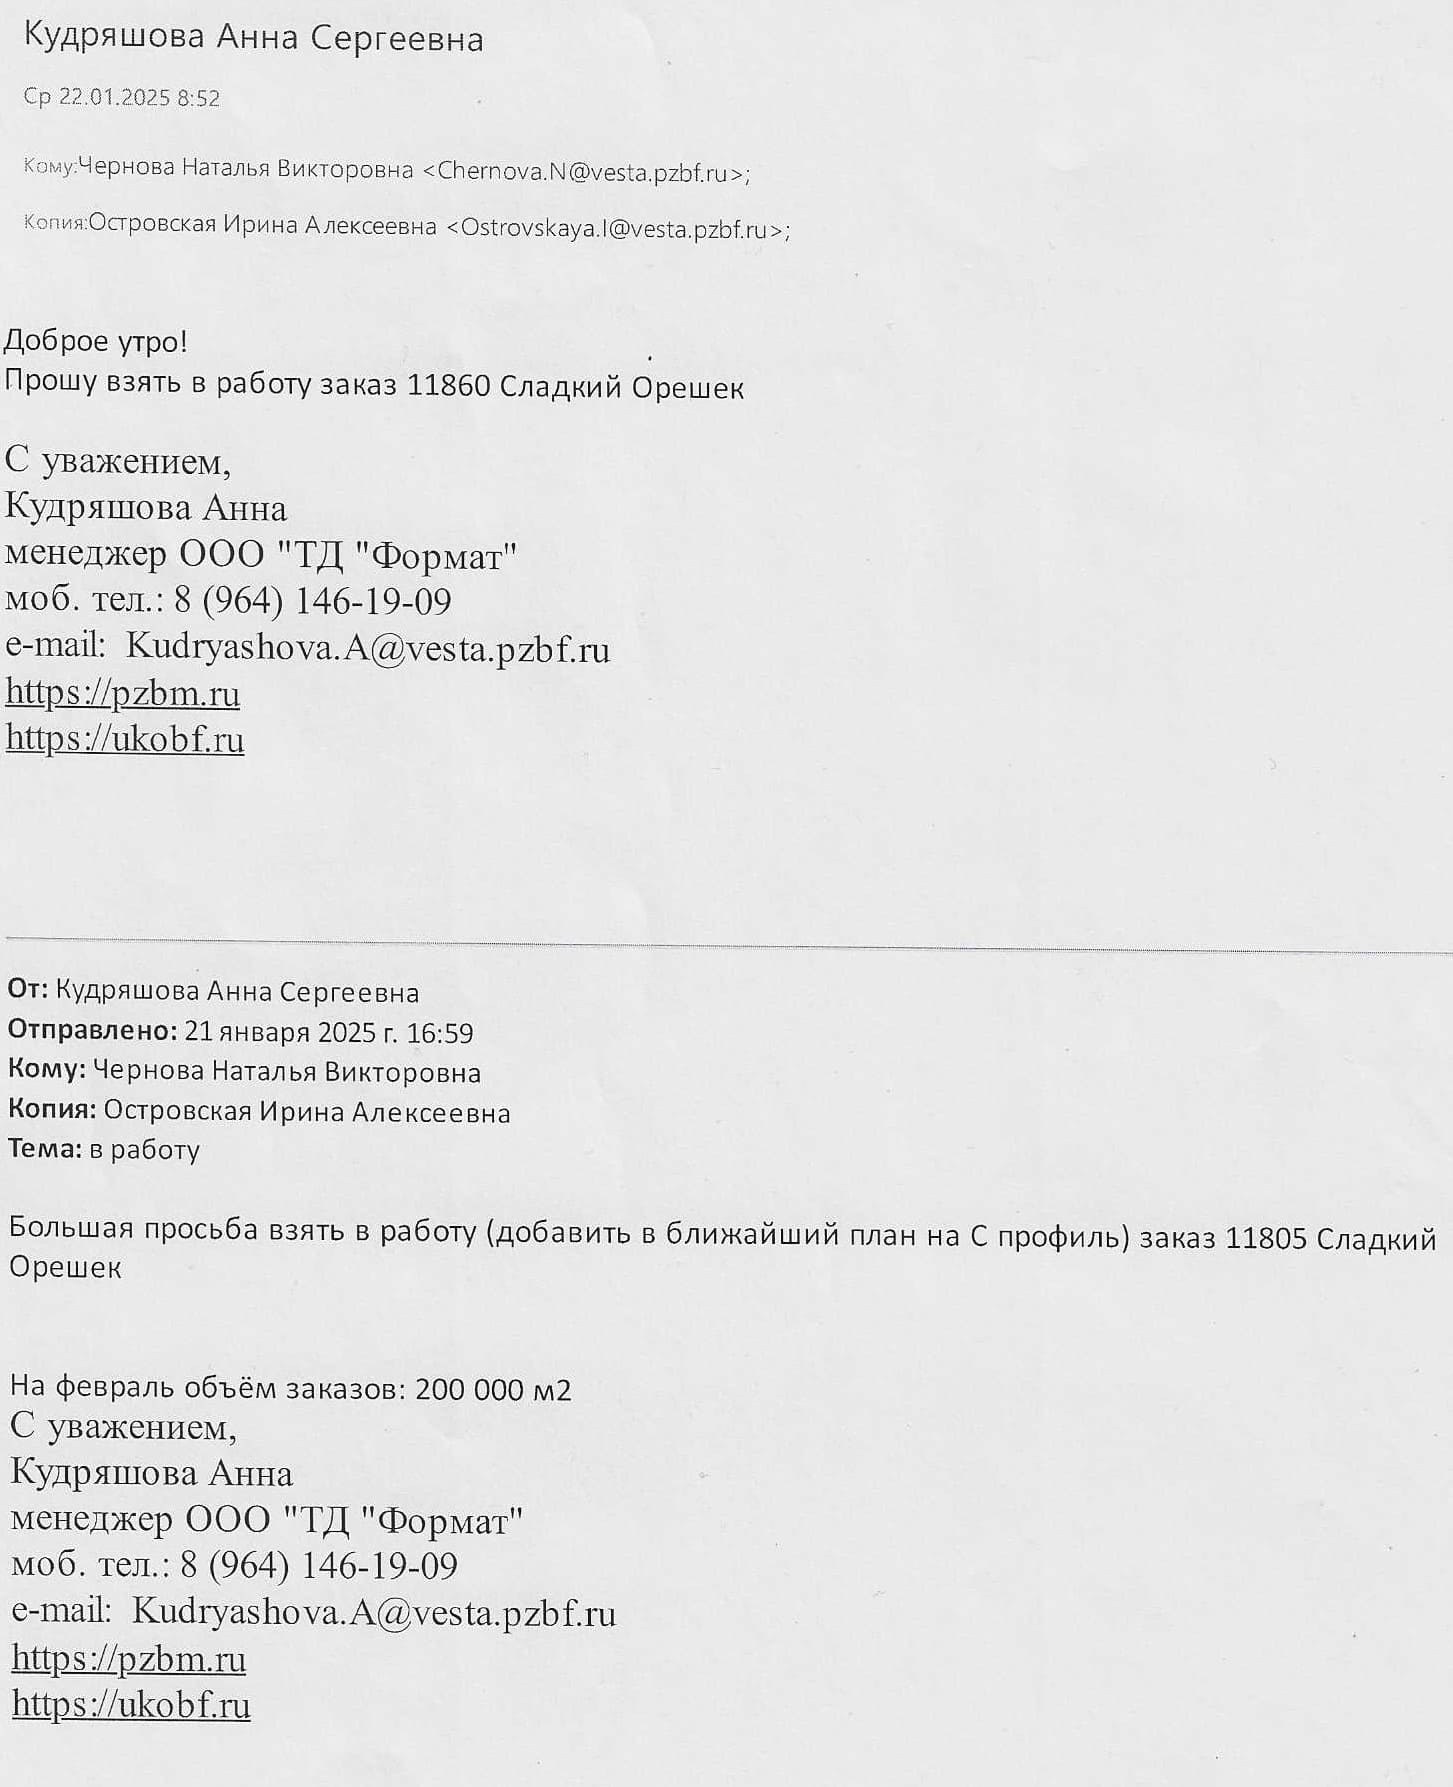
\includegraphics[height=0.7\textheight, keepaspectratio]{Pics/VII 1.jpg}
%\end{center}
%\caption{Сообщение отделу планирования о создании нового заказ}
%\label{pic:VII 1}
%\end{figure}
\clearpage

%Ежемесячно менеджеры отдела сбыта и логистики совместно с коммерческим директором разрабатывают оперативный план. 

% Разрез планирования: виды выпускаемой продукции, декада месяца.
% Показатель планирования: метры квадратные по готовой продукции.
 
%Позаказный учет отсутствует.
 
%Для каждой позиции указывается заказчик, размеры изделия, марка, оснастка, композиция сырья, план в производство и факт производства и отгрузки.

%План создается по каждому менеджеру. Оперативный план продаж является документом, по которому формируются все дальнейшие планы: план производства, план работы гофроагрегата, план работы перерабатывающих линий, план потребности в материалах, план отгрузки.
%Форма плана приведена на рис. \ref{pic:salesplan}.
%
% \begin{figure}
% \begin{center}
%  
\includegraphics[height=0.94\textheight, width=0.9\textwidth,  keepaspectratio]{Pics/Pattern.jpg}
% \end{center}
%  \caption{Форма заказа покупателя в системе СБИС}
%  \label{pic:d14}
% \end{figure}
% \clearpage


% \begin{figure}
% \begin{center}
%  \includegraphics[height=0.94\textheight, width=0.9\textwidth,  keepaspectratio]{Pics/pic.jpg}
% \end{center}
%  \caption{Цепочка заказов для планирования}
%  \label{pic:pic_d14}
% \end{figure}
% \clearpage

%
%



%Оперативное планирование определяется на основе формы \ref{pic:monthplan}, куда менеджер фиксирует все поступающие заявки.
%Производство каждый день  сообщает менеджерам коммерческого отдела  результаты работы производства. 
%При этом плановик  звонит менеджеру коммерческого отдела и говорит какие заказы приняты в производство на текущую дату.
%%Специалисты отдела планирования сообщают план выполнения на 2 дня. 
%Планировщик сообщает дату, на которую поставлен заказ. Так менеджеры узнают, когда их заявка покупателя поставлена в работу. 
%Дата (период) производства в форме плана  (см рис. \ref{pic:monthplan}) уже согласована.
%В программе 1С менеджер создает надокумент ''Счет''  и печатает форму заказа на отгрузку, в котором указывает дату отгрузки, адрес доставки, номенклатуру продукции, цены, объём. 


%\begin{figure}
%\begin{center}
%  \includegraphics[height=0.94\textheight, keepaspectratio]{Pics/prodline_loading.jpg}
%\end{center}
%  \caption{Отчет по загруженности линий}
%  \label{pic:prodline_loading}
%\end{figure}

%\clearpage
%\ifx \notincludehead\undefined
\normalsize
\end{document}
\fi
\newpage
\subsection{Расчет предварительной стоимости продукции}
\label{bp:calculation}

Расчет предварительной стоимости продукции производится в системе 1С: УПП. 

Менеджер собирает всю информацию от клиента по новому изделию. 
Менеджер получает требования от клиента, уточняет размеры, условия доставки, марки. Требования обычно приходят устно, через мессенджеры, по электронной почте.
Менеджер в системе 1С: УПП производит предварительный расчет стоимости продукции двумя способами:
\begin{enumerate}
    \item Создает документ ''Расчет стоимости продукции'' (рис. \ref{pic:I.2.4..jpg}) на основании предварительно сформированного им черновика ТК (рис. \ref{pic:II.4.jpg}) и с использованием кнопки ''Расчет стоимости'' и ''Расчет Маржи'' производит расчет.
    \item Не формируя ТК создает документ ''Расчет стоимости продукции'', заполняет все необходимые характеристики. Далее производит расчет с использованием кнопок ''Расчет стоимости'' и ''Расчет Маржи''.
\end{enumerate}

В некоторых случаях менеджер может завысить расчетную стоимость изделия. 

Результаты расчетов согласовываются с коммерческим отделом ООО ТД ''ФОРМАТ'' и только после согласования оформляется Коммерческое предложение (рис. \ref{pic:I.4.jpg}).
Заказчик ответным письмом высылает менеджеру согласованное предложение, указывает свои реквизиты 
% (рис. \ref{pic:I.2.1.jpg}) 
для заключения договора. 
% Менеджер при необходимости может запросить дополнительную информацию (рис. \ref{pic:I.2.2.jpg}), необходимую для заключения договора.

Весь внутренний документооборот фиксируется в программе ''Первая Форма'' (рис. \ref{pic:I.5.2..jpg}).
Учет договоров с контрагентами осуществляется в системе 1С: УПП.
После согласования проекта договора через программу ''Первая Форма'' менеджер должен создать заявку на заведение нового контрагента (рис. \ref{pic:I.5.2.jpg}) в системе 1С: УПП.
Нового контрагента в систему 1С: УПП заводит Бухгалтерия.

Оригиналы подписанных договоров хранятся в бухгалтерии.






%Менеджер выполняет расчет предварительной цены продажи в таблице MS Excel (рис. \ref{pic:dd5}), подбирает параметры. Цена указывается за м2 по марке картона. Четкого алгоритма расчета цены продажи не выявлено.


%Цены по стоимости за марку картона зафиксированы за 2 месяца в таблице MS Excel  (рис. \ref{pic:dd3}). Коммерческий директор выполняет расчет цены в форме файл \ref{pic:dd3} и выкладывает цены в сетевой доступ для менеджеров. Менеджер добавляет в цену расчет на упаковку, доставку и получает цену продажи.
%Менеджер формирует КП (рис. \ref{pic:dd4}). Шаблона четкого нет. 

%Менеджер высылает коммерческое предложение клиенту.  Заказчик в ответ высылает менеджеру согласованное предложение с реквизитами для заключения договора. 
%Менеджер формирует договор поставки и высылает заказчику на согласование.

%После согласования коммерческого предложения Менеджер 
%создает вручную проект договора (рис. \ref{pic:dd5}), создает карточку договора в системе СБИС.

%Номер договора присваивает юрист по запросу менеджера. Менеджер в системе СБИС создает спецификацию по клиенту, заводит в справочник Номенклатура в СБИС новую позицию, указывает размеры, площадь, тип гофры, цвет картона, размеры упаковки .
%Система СБИС присваивает номенклатурный номер.
%Менеджер заполняет спецификацию в СБИС (рис. \ref{pic:dd6_1}). Менеджер в СБИС ставит в обработку (фиксирует), печатает спецификацию в СБИС (рис. \ref{pic:dd6_1}). Менеджер создает бланк договора и спецификацию в системе СБИС. 
%Менеджер создает счет в СБИС. Номенклатура выбирается по созданной спецификации. 
%Менеджер печатает счет на оплату (рис. \ref{pic:dd8}).

%Менеджер отправляет клиенту договор с приложением в виде спецификации, счет на предоплату при необходимости.
%Клиент подписывает договор, спецификацию и оплачивает счет.



%После согласования цены Менеджер должен начать разработку ТК (см. процесс ''Подготовка производства'' \ref{bp:Prepare}).




% \begin{figure}
% \begin{center}
% 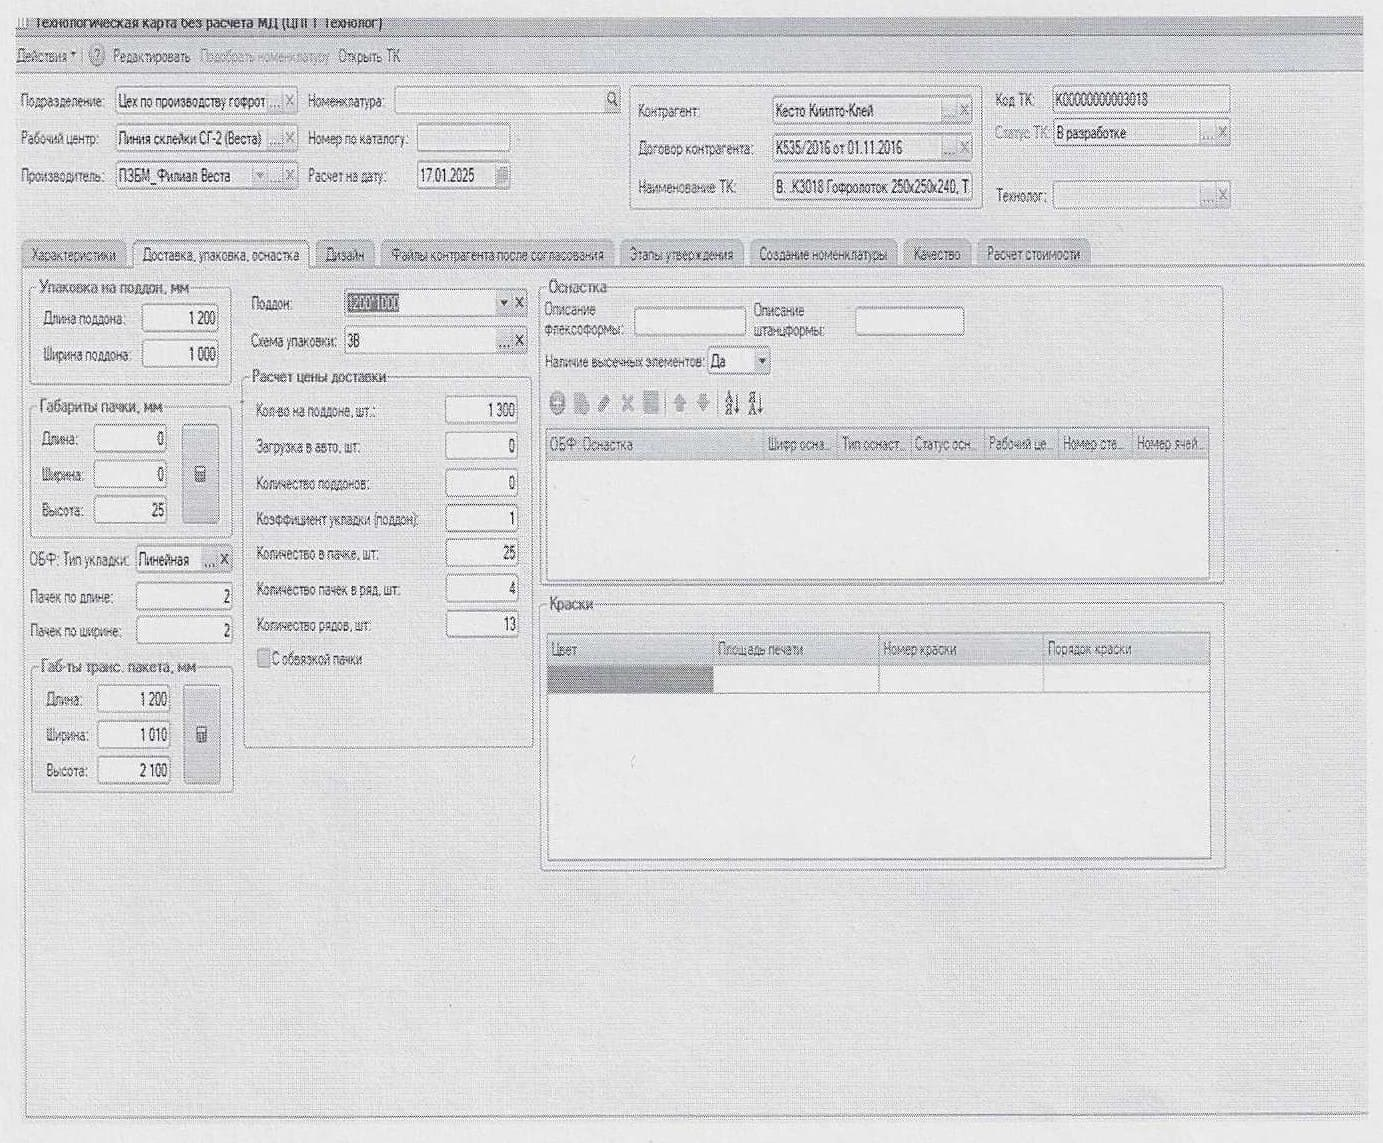
\includegraphics[height=0.5\textheight, width=1.3\textwidth, keepaspectratio]{Pics/II.4.jpg}
% \end{center}
% \caption{Форма Технологическая карта}
% \label{pic:II.4.jpg}
% \end{figure}
% \clearpage

\begin{figure}
\begin{center}
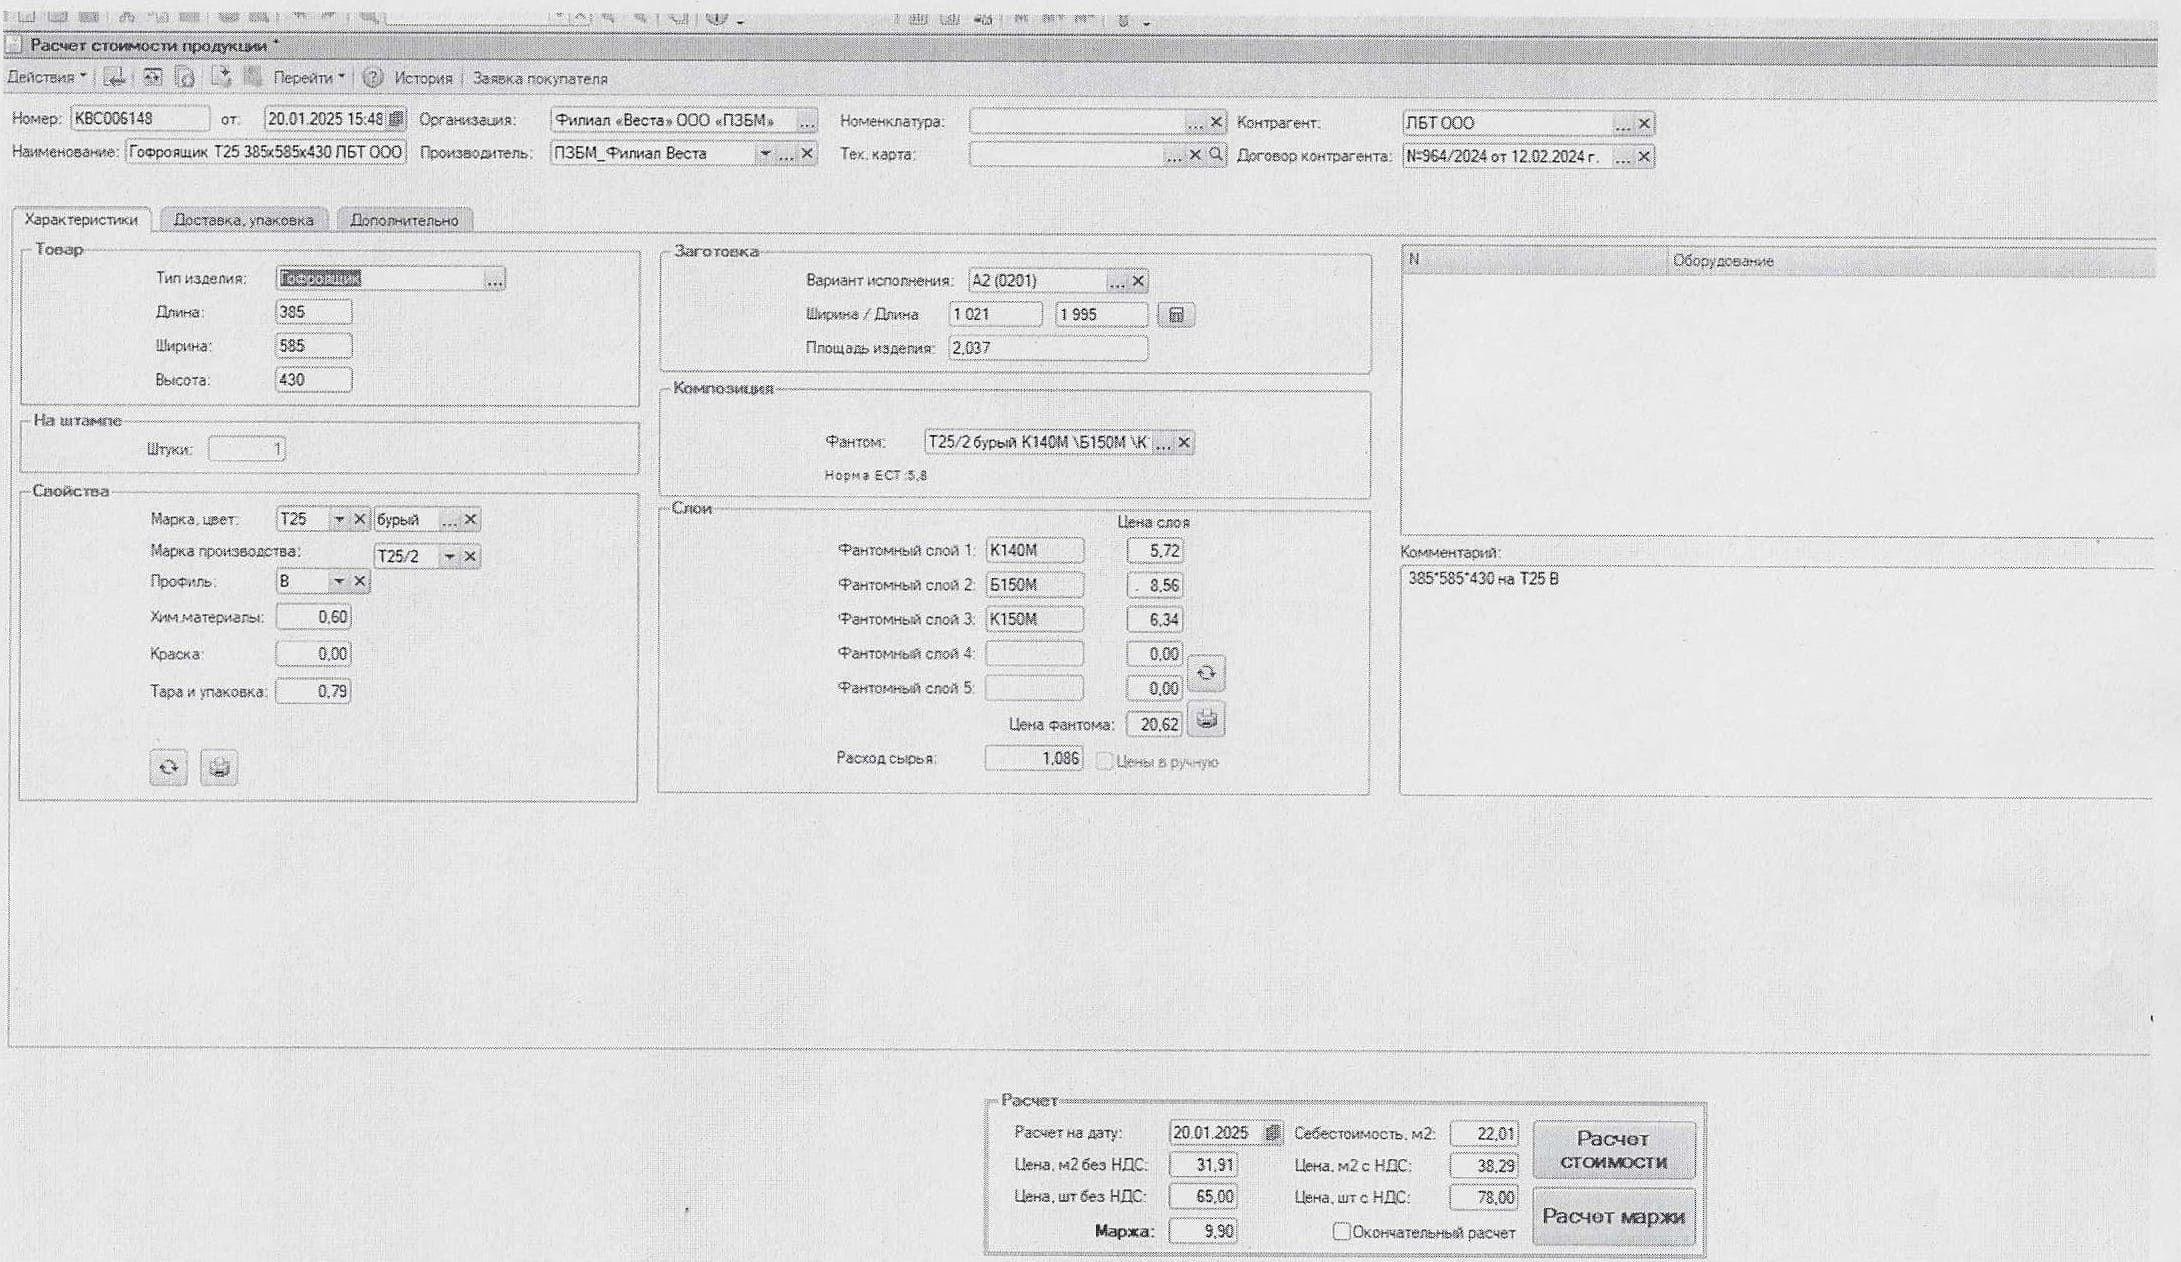
\includegraphics[height=0.38\textheight, width=1.3\textwidth, keepaspectratio]{Pics/I.2.4..jpg}
\end{center}
\caption{Расчет стоимости продукции}
\label{pic:I.2.4..jpg}
\end{figure}
\clearpage

\begin{figure}
\begin{center}
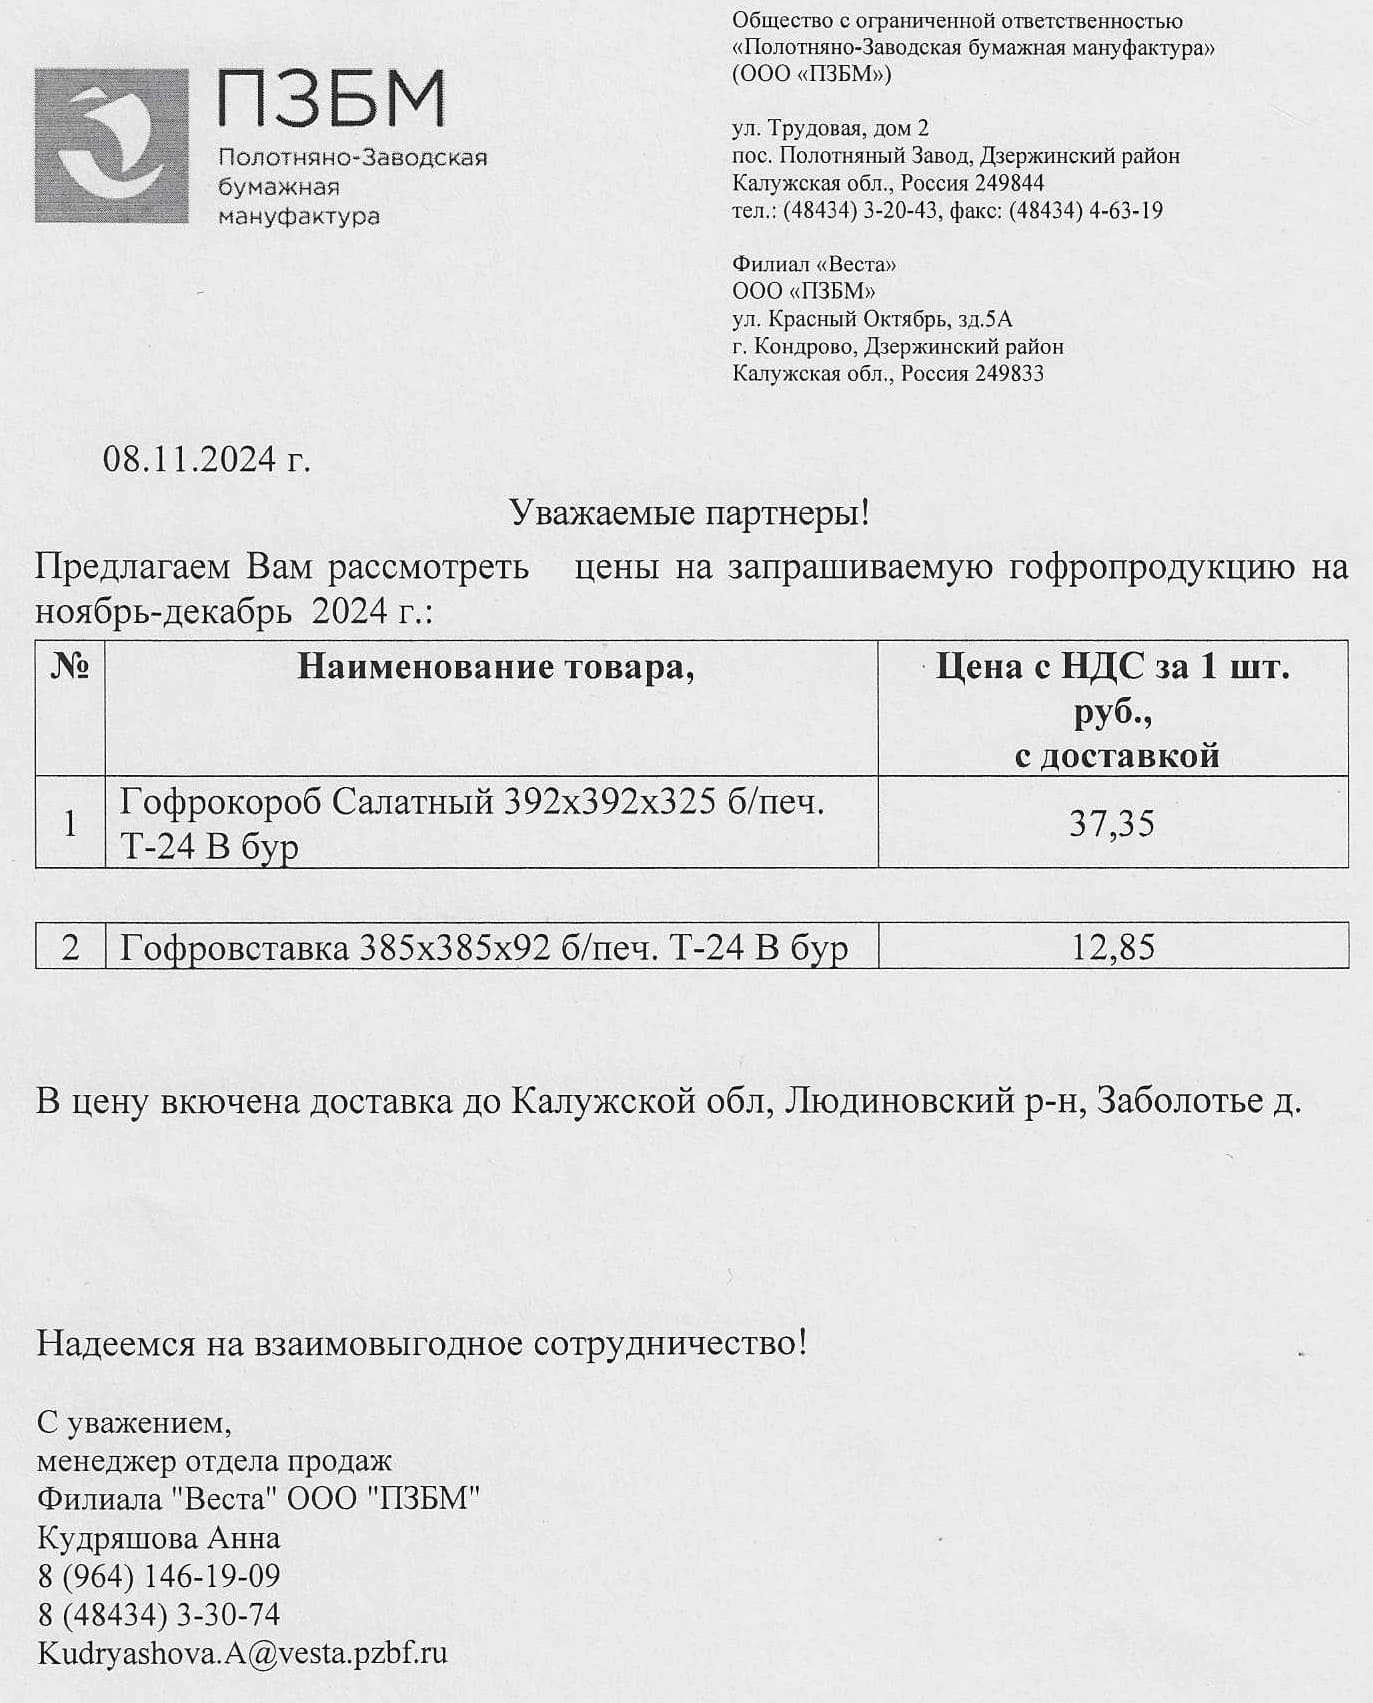
\includegraphics[height=0.8\textheight, width=1.5\textwidth, keepaspectratio]{Pics/I.4.jpg}
\end{center}
\caption{Пример Коммерческого предложения}
\label{pic:I.4.jpg}
\end{figure}
\clearpage

% \begin{figure}
% \begin{center}
% 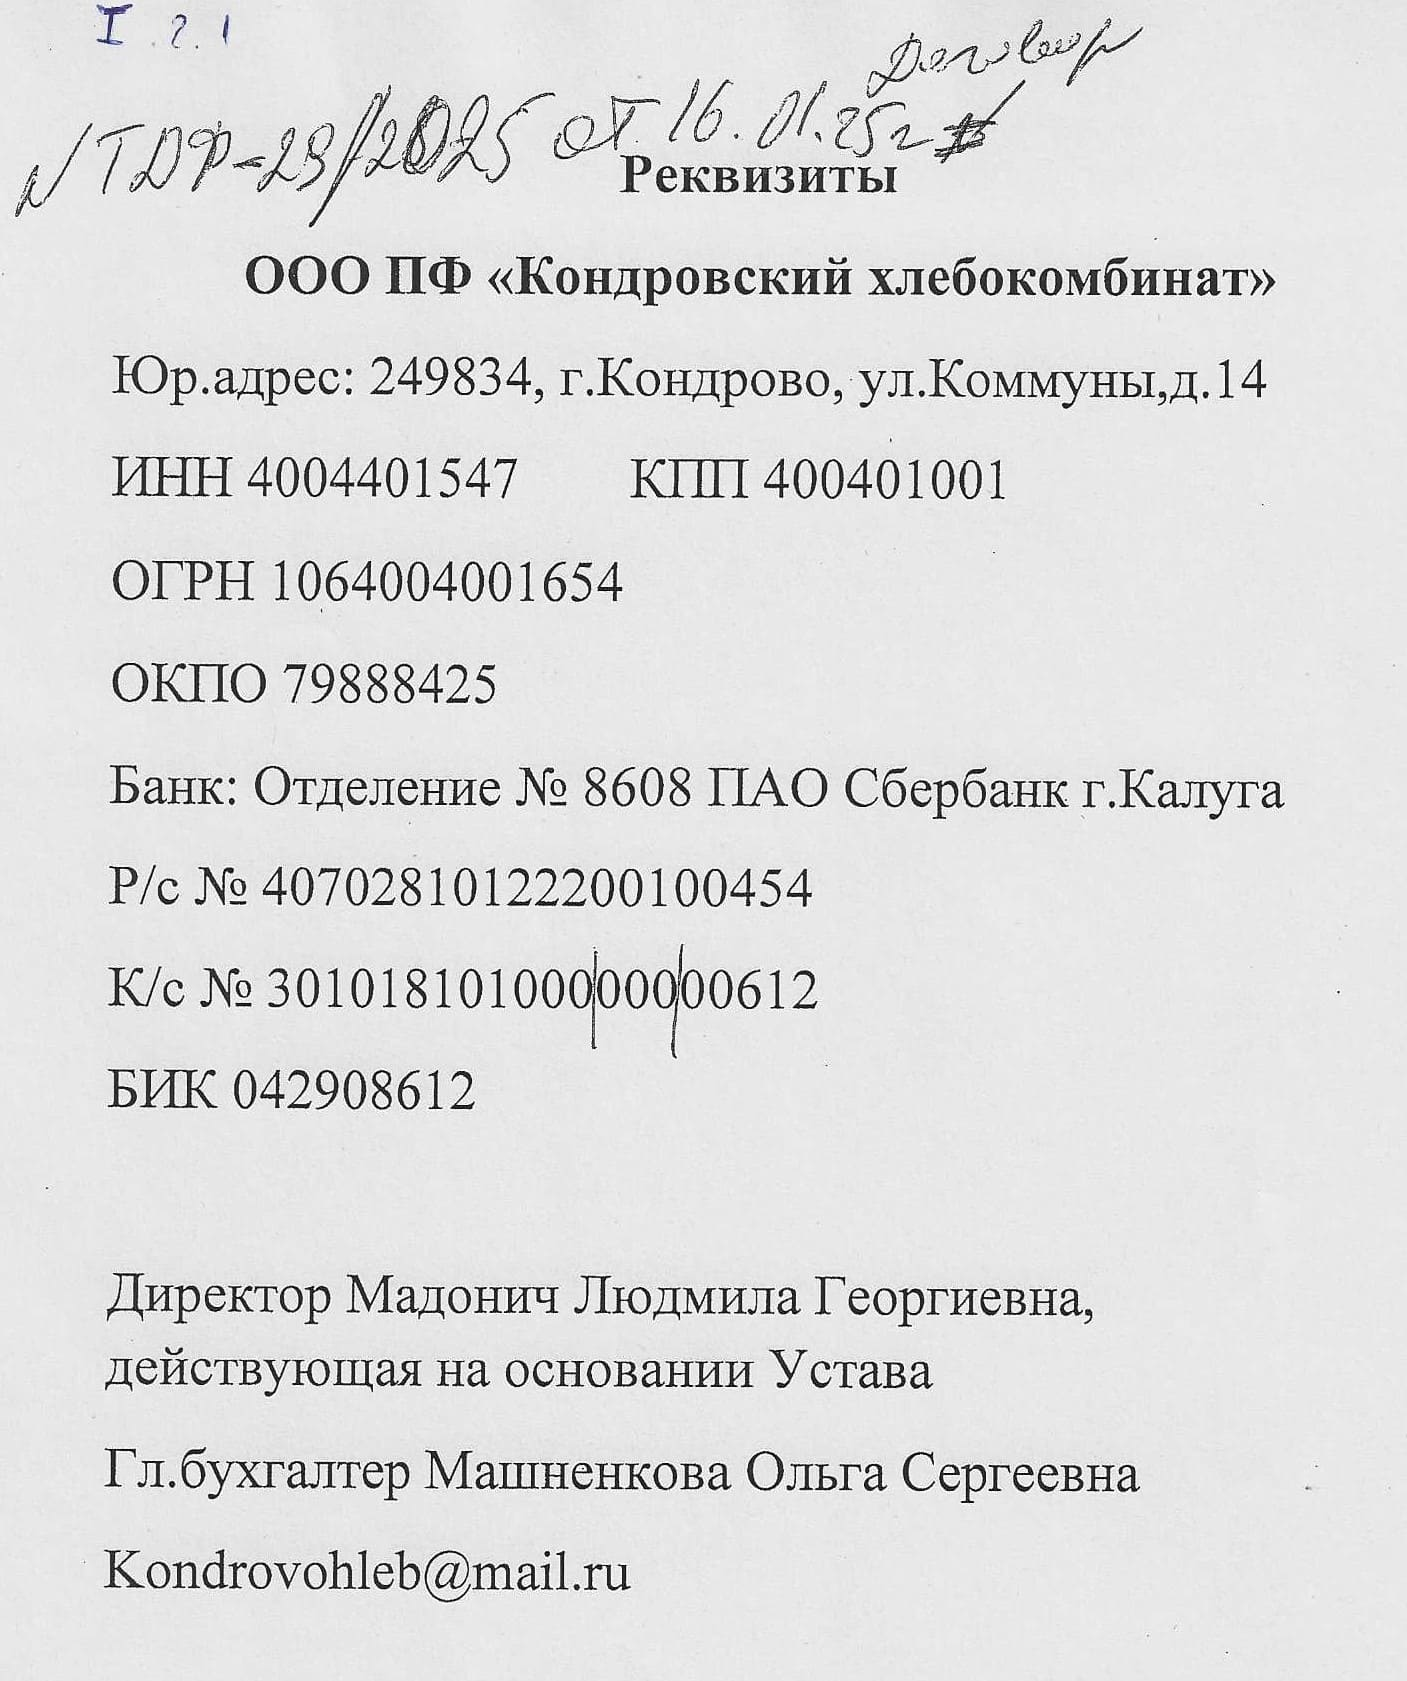
\includegraphics[height=0.6\textheight, width=1.5\textwidth, keepaspectratio]{Pics/I.2.1.jpg}
% \end{center}
% \caption{Пример реквизитов заказчика}
% \label{pic:I.2.1.jpg}
% \end{figure}
% \clearpage

% \begin{figure}
% \begin{center}
% 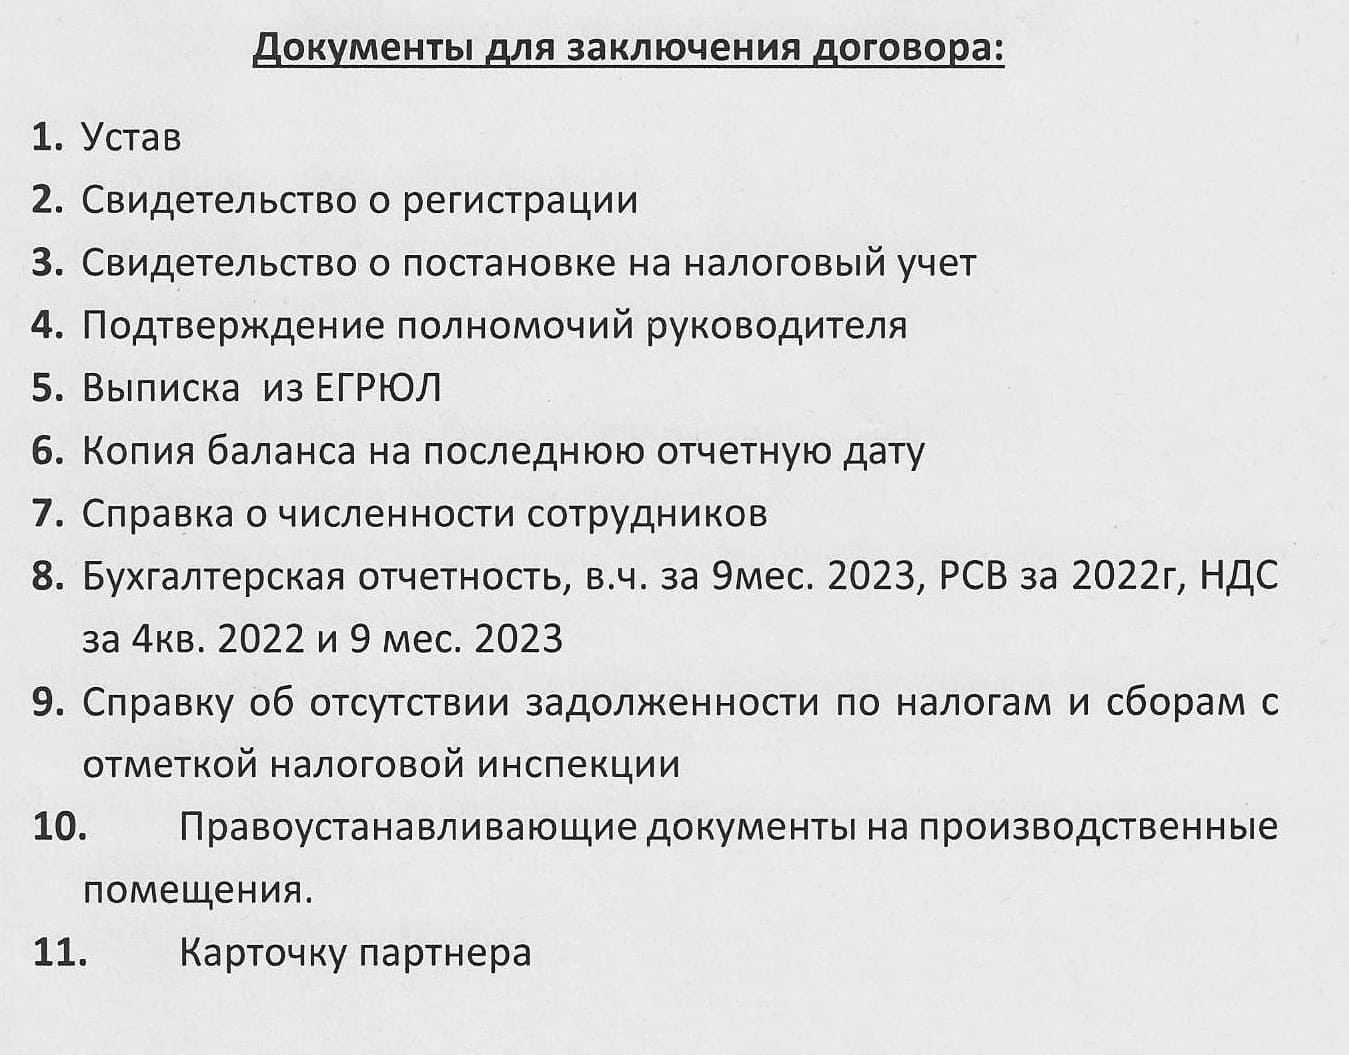
\includegraphics[height=0.45\textheight, width=1.5\textwidth, keepaspectratio]{Pics/I.2.2.jpg}
% \end{center}
% \caption{Требуемые документы для заключения договора}
% \label{pic:I.2.2.jpg}
% \end{figure}
% \clearpage


\begin{figure}
\begin{center}
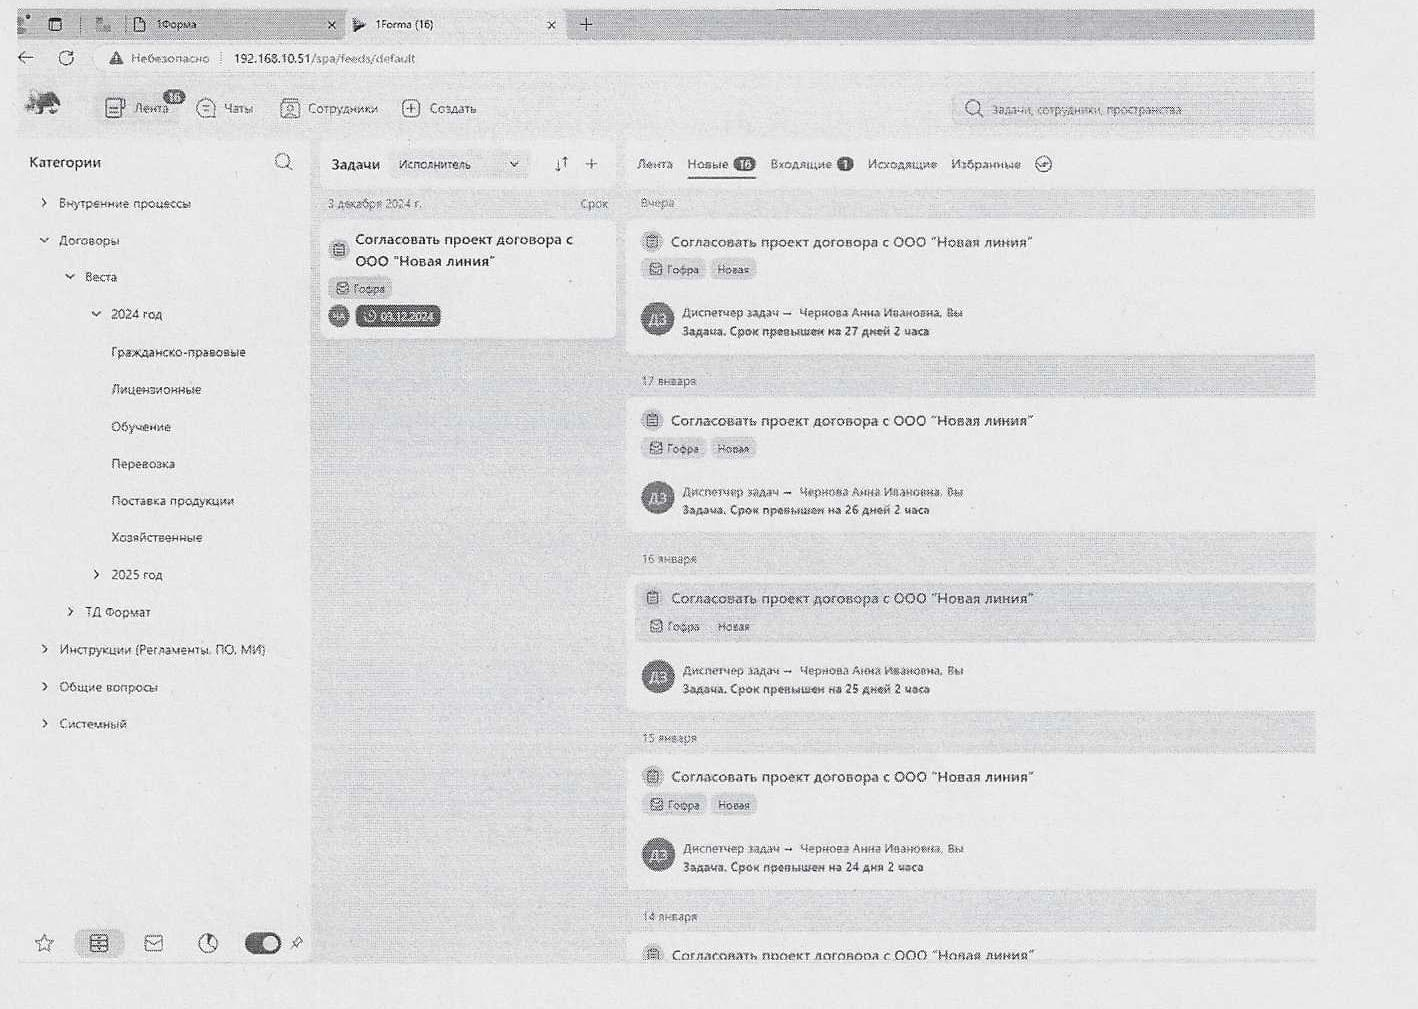
\includegraphics[height=0.45\textheight, width=1.5\textwidth, keepaspectratio]{Pics/I.5.2..jpg}
\end{center}
\caption{Программа ''Первая форма''}
\label{pic:I.5.2..jpg}
\end{figure}
\clearpage

\begin{figure}
\begin{center}
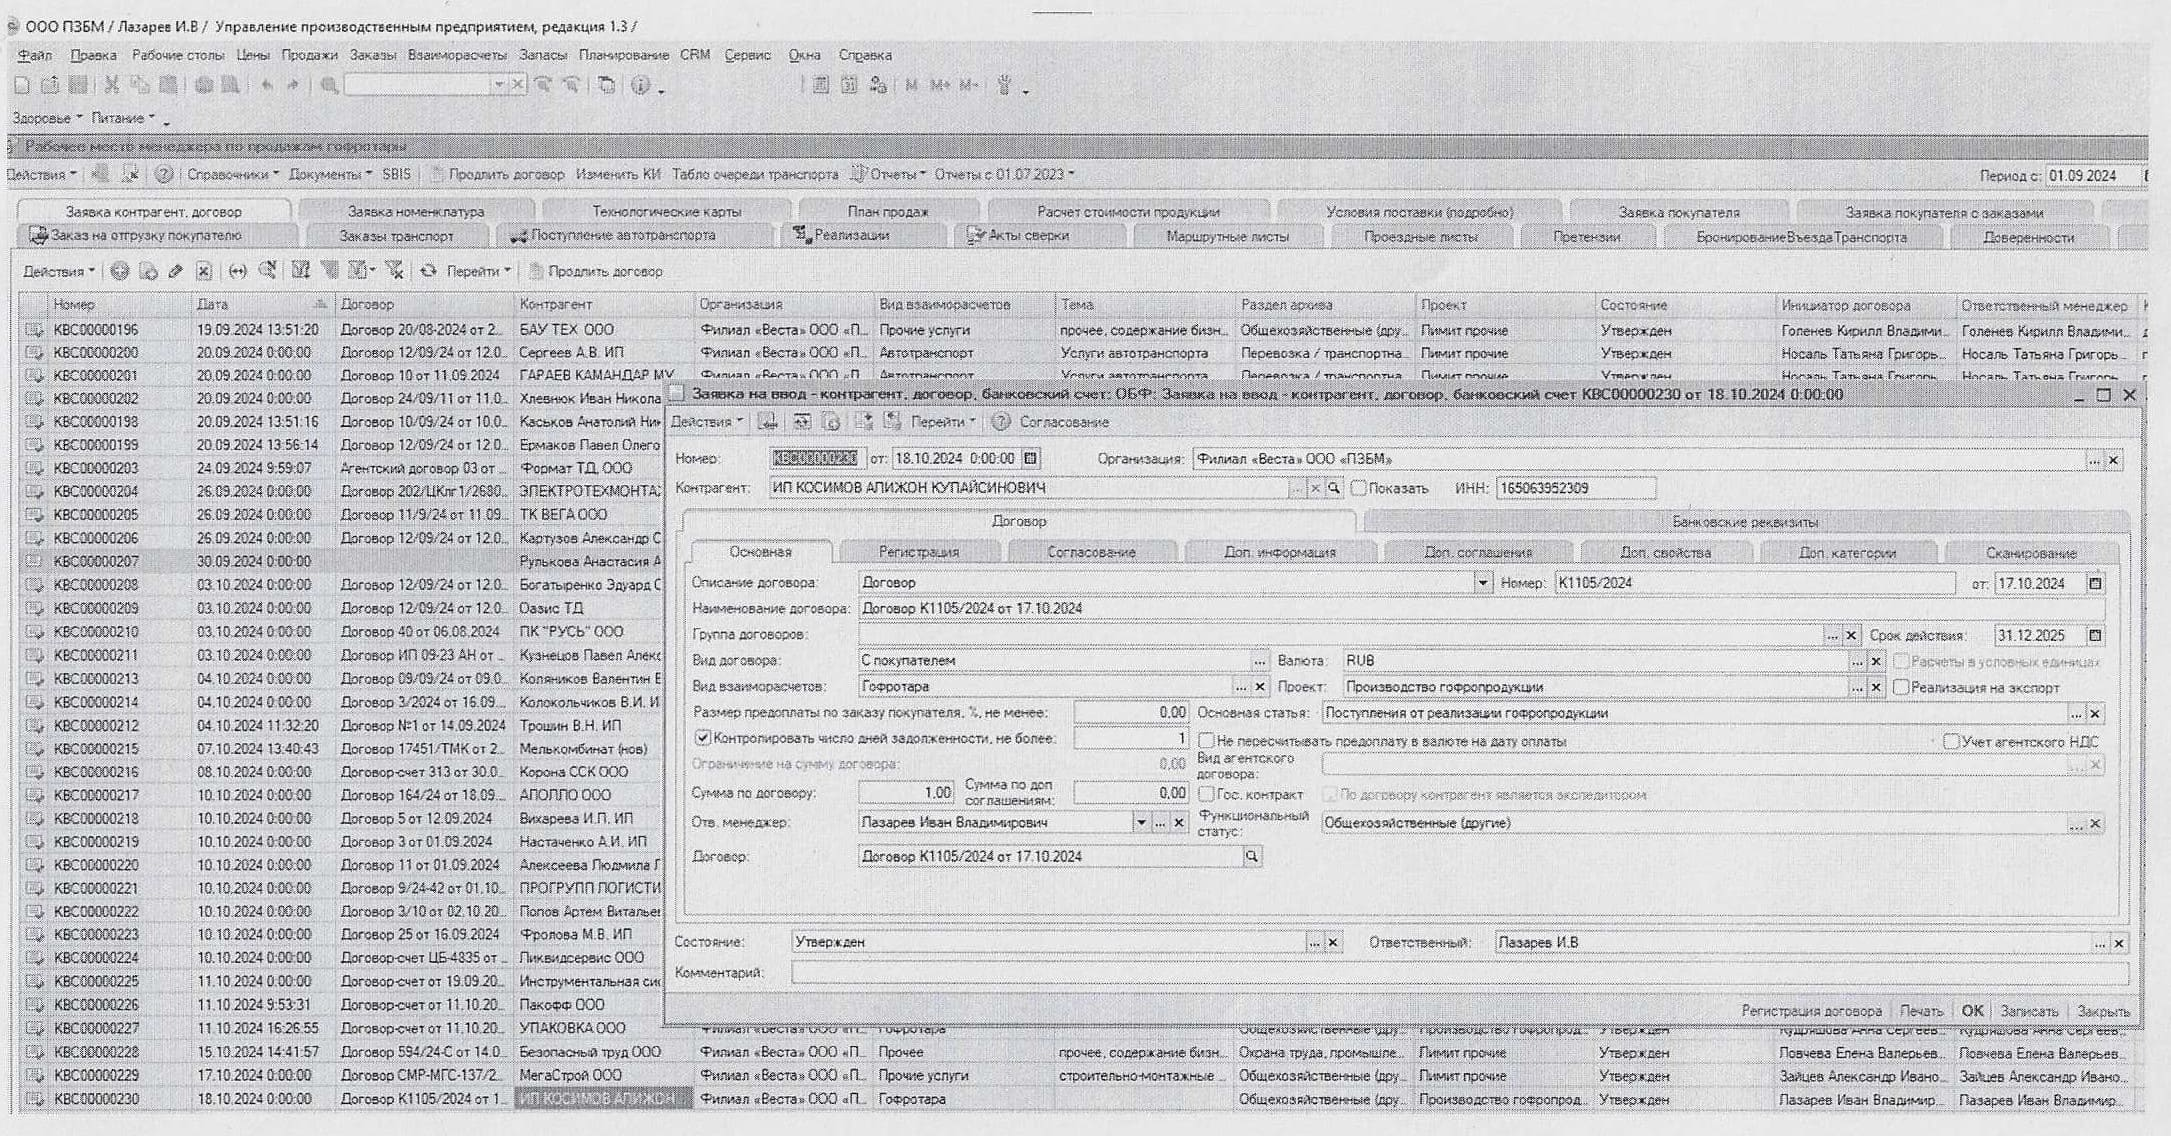
\includegraphics[height=0.35\textheight, width=1.5\textwidth, angle=90, keepaspectratio]{Pics/I.5.2.jpg}
\end{center}
\caption{Форма заявки на ввод нового контрагента в 1С: УПП}
\label{pic:I.5.2.jpg}
\end{figure}
\clearpage

% Для расчета цены менеджер использует шаблон в MS Excel (рис. \ref{pic:pic_d2}). 
% К цене сырья добавляется стоимость на сложную высечку.  Стоимость упаковки включена в цену изделия. Таким образом менеджер определяет базовую нормативную себестоимость продукции.  Цена продажи определяется менеджером исходя из себестоимости и рентабельности производства.


% Каждый менеджер ведет расчет по новым изделиям в своих файлах. Менеджер заносит в файл наименование изделия (обычно контрагент) длину, ширину, высоту (внутренние размеры изделия). По формуле будет рассчитана площадь изделия. Менеджер выбирает сырье по композиции. 
% Менеджер подбирает сырье по аналогии либо по истории такой же коробки. 

% При необходимости изготовления сложной высечки менеджер  запрашивает у контрагента чертеж или образец (процесс ''Изготовление образцов продукции'' \ref{bp:pattern}).

% На основании расчета (рис. \ref{pic:pic_d2}) менеджер формирует коммерческое предложение (рис. \ref{pic:pic_d3}). Для печати предложения используется шаблон.
% На основе полученного результата расчета себестоимости изделия менеджер  формирует коммерческое предложение и высылает его заказчику (рис. \ref{pic:pic_d3}). Для печати предложения используется шаблон. Номер КП указывается по порядку. В коммерческом предложении указывается наименование гофропродукции, марка, профиль и цена изделия. Цена актуальна в течение месяца. 
% Коммерческое предложение высылается заказчику для согласования.
% Все предложения менеджер фиксирует в таблице MS Excel предложения  (рис. \ref{pic:pic_d4}).


% Менеджер высылает КП заказчику.
% Заказчик высылает менеджеру согласованное предложение с реквизитами для заключения договора. Менеджер формирует договор поставки и высылает заказчику на согласование. В дополнение к договору менеджер формирует спецификацию на цену продукции, где указывается согласованный перечень поставляемой продукции и цены на нее (рис. \ref{pic:pic_d5}). Дополнительное соглашение является дополнением к договору. Все документы заполняются менеджером вручную.
% После согласования заказчиком коммерческого предложения менеджер запрашивает карточку контрагента для заключения договора. Менеджер отправляет в офис Московский карточку контрагента и спецификацию (рис. \ref{pic:pic_d5}) для заключения договора.

% Секретарь формирует договор с заказчиком, присваивает номер дату и высылает договор менеджеру по электронной почте. Менеджер согласует договор с заказчиком. Заказчик подписывает договор. Менеджер передает в бухгалтерию карточку заказчика и копию подписанного договора. 
% Отдел учета в системе 1С Предприятие 7.7 Бухгалтерия  создаёт  справочнике ''Контрагенты'' нового заказчика и договор.

% После выставления счета менеджер контролирует оплату от заказчика. Контроль оплаты менеджер выполняет в программе 1С 7.7. Бухгалтерия. В системе 1С 8.3 ''Бухгалтерия предприятия'' ведётся  учет поступления денежных средств на расчётный счёт, но с опозданием.
% Банк ведется в двух системах: 1С 7.7. Бухгалтерия и 1С 8.3 ''Бухгалтерия предприятия''.


%Менеджер получает запрос только по почте менеджер создает заявку на расчёт \ref{pic:calculation1}.
%Менеджер звонит на производство специалисту по планированию, который присваивает номер гофроизделия в файле ''Начало''.
%Менеджер подбирает сырье для производства изделия самостоятельно, при это есть таблица компоновок сырья \ref{pic:Layerscost}, которая не используется. Менеджер определяет количество на поддоне. При указании вида транспорта менеджер рассчитывает стоимость доставки \ref{pic:transportcost}. Менеджер рассчитывает количество поддонов, чтобы посчитать затраты на доставку. Особые условия указанной в условиях упаковке.
%
%Файл  \ref{pic:calculation1} отправляется экономисту почтой. 
%
% Расчет предварительной стоимости изделия выполняет МАП в системе 1С:УНФ при получении заявки от покупателя. Цена для продажи рассчитывается исходя из суммы следующих слагаемых.
% \begin{itemize}
% \item Стоимость гофрокартона -- рассчитывается как стоимость одного метра гофрокартона определенного профиля.
% \item Наценка за печать -- менеджер указывает примерную площадь запечатки краской в процентах. Процент запечатки учитывается при расчете затрат на печать.
% \item Паллетирование -- если для изделия требуется укладка на поддон, то стоимость паллетирования добавляется в стоимость изделий. Стоимость паллетирования одного изделия рассчитывается как стоимость паллетирования одного поддона, деленная на количество изделий на поддоне.
% \item Затраты на упаковку;
% \item Транспортировка -- стоимость доставки готовой продукции до получателя на единицу продукции.
% \end{itemize}
%
%
% \begin{figure}
% \begin{center}
%   \includegraphics[width=\linewidth, height=0.94\textheight, keepaspectratio]{Pics/d1.jpg}
% \end{center}
%   \caption{Форма расчета стоимости нового изделия}
%   \label{pic:d1}
% \end{figure}
% \clearpage
%
%
% \begin{figure}
% \begin{center}
%   \includegraphics[width=\linewidth, height=0.94\textheight, keepaspectratio]{Pics/d5.jpg}
% \end{center}
%   \caption{Форма коммерческого предложения}
%   \label{pic:d5}
% \end{figure}
% \clearpage

%
%%
% \begin{figure}
% \begin{center}
%   \includegraphics[width=\linewidth, height=0.94\textheight, keepaspectratio]{Pics/d5.jpg}
% \end{center}
%   \caption{Форма коммерческого предложения}
%   \label{pic:d3}
% \end{figure}
% \clearpage


% \begin{figure}
% \begin{center}
%   \includegraphics[width=\linewidth, height=0.94\textheight, keepaspectratio]{Pics/d6.jpg}
% \end{center}
%   \caption{Форма спецификации к договору}
%   \label{pic:d6}
% \end{figure}
% \clearpage

% \begin{figure}
% \begin{center}
%   \includegraphics[width=\linewidth, height=0.94\textheight, keepaspectratio]{Pics/pic_d5.jpg}
% \end{center}
%   \caption{Форма спецификации к договору}
%   \label{pic:pic_d5}
% \end{figure}
% \clearpage

%
%\begin{figure}
%\begin{center}
%\ifnum\pdfoutput=0
%  \includegraphics[40,0][366,292]{Pics/03_calculation2.png}
%\else 
%  \includegraphics[width=\linewidth, height=0.94\textheight, keepaspectratio]{Pics/03_calculation2.jpg}
%\fi
%\end{center}
%  \caption{Расчет стоимости изделия от экономиста.}
%  \label{pic:calculation2}
%\end{figure}
%\clearpage
%
%
%\begin{figure}
%\begin{center}
%\ifnum\pdfoutput=0
%  \includegraphics[40,0][366,292]{Pics/03_calculation3.png}
%\else 
%  \includegraphics[width=\linewidth, height=0.94\textheight, keepaspectratio]{Pics/03_calculation3.jpg}
%\fi
%\end{center}
%  \caption{Упрощенный расчет стоимости.}
%  \label{pic:calculation3}
%\end{figure}
%\clearpage
%
%
%

%
%
%\begin{figure}
%\begin{center}
%\ifnum\pdfoutput=0
%  \includegraphics[40,0][366,292]{Pics/04_KP1.png}
%\else 
%  \includegraphics[width=\linewidth, height=0.94\textheight, keepaspectratio]{Pics/04_KP1.jpg}
%\fi
%\end{center}
%  \caption{Коммерческое предложение.}
%  \label{pic:KP1}
%\end{figure}
%\clearpage
%
%
%\begin{figure}
%\begin{center}
%\ifnum\pdfoutput=0
%  \includegraphics[40,0][366,292]{Pics/34_contract.png}
%\else 
%  \includegraphics[width=\linewidth, height=0.94\textheight, keepaspectratio]{Pics/34_contract.jpg}
%\fi
%\end{center}
%  \caption{Договор поставки.}
%  \label{pic:contract}
%\end{figure}
%\clearpage
%
%
%\begin{figure}
%\begin{center}
%\ifnum\pdfoutput=0
%  \includegraphics[40,0][366,292]{Pics/07_specification_for_contract.png}
%\else 
%  \includegraphics[width=\linewidth, height=0.94\textheight, keepaspectratio]{Pics/07_specification_for_contract.jpg}
%\fi
%\end{center}
%  \caption{Спецификация к договору поставки.}
%  \label{pic:specificationforcontract}
%\end{figure}
%\clearpage
%
%
%
%
%
%
%
%
%
%
%%Расчет предварительной стоимости изделия выполняется в отделе маркетинга при получении заявки от покупателя.
%%
%%Технолог ОМ заполняет таблицу по расчету предварительной себестоимости изделия (см. рис.\ref{pic:Calculation}. Экономист в структуре ОМ выполняет по данному расчету расчет себестоимости изделия для покупателя. Для расчета используются нормативные цены для расчета стоимости изделия (рис. \ref{pic:Compound},  \ref{pic:CompoundPrint}, \ref{pic:CalculationPack}, \ref{pic:CompoundPrint}).
%%
%%На основе полученного результата расчета себестоимости изделия менеджер ОМ формирует коммерческое предложение и высылает заказчику. Согласованное заказчиком предложение с реквизитами для заключения договора покупатель высылает в ОМ. Менеджер передает заявку юристу для составления и согласования договора. Экономист в структуре ОМ формирует спецификацию к договору. В спецификации указывается условия производства, отгрузки и поставки продукции (рис. \ref{pic:Offer}).
%%
%%На основании согласованной с заказчиком и подписанной заявки технологи ОМ разрабатывают технологическую карту изделия (см. процесс ''Подготовка производства'' \ref{bp:Prepare}).
%
%%\begin{figure}
%%\begin{center}
%%  \includegraphics[height=0.94\textheight, keepaspectratio]{Pics/Calculation.jpg}
%%\end{center}
%%  \caption{Форма заполнения расчета для нового изделия}
%%  \label{pic:Calculation}
%%\end{figure}

% \clearpage
% \begin{figure}
% \begin{center}
%  \includegraphics[height=0.7\textheight, keepaspectratio]{Pics/dd5.jpg}
% \end{center}
%  \caption{Карточка организации в СБИС}
%  \label{pic:dd5}
% \end{figure}


% \begin{figure}
% \begin{center}
%  \includegraphics[height=0.5\textheight, keepaspectratio]{Pics/dd3.jpg}
% \end{center}
%  \caption{Форма расчета цены готовой продукции}
%  \label{pic:dd3}
% \end{figure}

% \begin{figure}
% \begin{center}
%  \includegraphics[height=0.94\textheight, keepaspectratio]{Pics/dd4.jpg}
% \end{center}
%  \caption{Форма коммерческого предложения}
%  \label{pic:dd4}
% \end{figure}
% \begin{figure}
% \begin{center}
%  \includegraphics[height=0.3\textheight, keepaspectratio]{Pics/dd6_1.jpg}
% \end{center}
%  \caption{Форма карточки номенклатуры готовой продукции}
%  \label{pic:dd6_1}
% \end{figure}


% \begin{figure}
% \begin{center}
%  \includegraphics[height=0.4\textheight, keepaspectratio]{Pics/dd8.jpg}
% \end{center}
%  \caption{Форма счета}
%  \label{pic:dd8}
% \end{figure}


% %
% \clearpage
% \ifx \notincludehead\undefined
\normalsize
\end{document}
\fi
\newpage
\subsection{Управление продажами}
\label{bp:SalesManagment}


Контроль за выполнением плана продаж осуществляет коммерческий отдел ООО ТД ''ФОРМАТ''.

Данные о потенциальных и существующих клиентах хранятся у каждого менеджера отдельно.
Каждый, действующий контрагент закреплен за конкретным менеджером. 

Все менеджеры отдела продаж на ПРЕДПРИЯТИИ фиксируют заявки и заказы в системе 1С: УПП. В заказе покупателя менеджер указывает условия вывоза: самовывоз или доставка производителем.
При формировании плана отгрузок заказы могут дробиться.

Менеджер контролирует складские остатки ГП.

При создании заказа покупателя менеджер проверяет дебиторскую задолженность в системе 1С: УПП. Менеджер пользуется системой электронного документооборота, в которой есть напоминание о финансовом положении клиента.

Менеджеры видят информацию по оплате покупателей в системе 1С: УПП. Каждый менеджер при необходимости обзванивает должников.



% % Менеджер заказывает заготовки точно под требуемый объем продукции и в нужный размер под готовую продукцию.
% На каждый заказ производства есть только одна заготовка.
% %Менеджер создает заказ на сторону только исходя из объема заказа на производство.
% Заказ заготовок создается точно по объему готовой продукции без дополнительных заготовок на пусконаладку. Отклонения в объеме готовой продукции прописаны в спецификациях к договору.
% % Дополнительные заготовки на пусконаладку не закупаются.
% Каждый МСЗ на основании заказа покупателя формирует заказ заготовок кратно транспортной единице (Фура). На предприятии заказывают до 12 фур в неделю заготовок. МСЗ считает загрузку транспорта вручную. Отгрузка продукции и заготовок осуществляется строго на паллетах.

% Каждое утро в 9-00 бухгалтер присылает выписки из банка. Менеджеры видят информацию по оплате покупателей в системе 1С:УНФ. Каждый менеджер при необходимости обзванивает должников. 


% Коммерческий директор ведет анализ продаж по событиям в системе 1С:УНФ.

% Покупатель может прислать дополнительную заявку кроме месячного плана.
%Все поступающие заявки менеджер фиксируют в файле “План” (рис. \ref{pic:monthplan}).

%
%Менеджер может разбить заявку покупателя на части с учётом загрузки в транспорт. 

%Менеджер печатает заявку покупателя по форме \ref{pic:SalesOrder}. В форме \ref{pic:SalesOrder} есть три экземпляра: один остается у менеджера, один передается на планирование переработки, один передается на планирование раскроя.   


%Заявку распечатанную в формате MS Excel менеджер передает экономисту для проверки задолженности. Экономист ставит свой штамп на бланке при одобрении заявки. Подписанную заявку менеджер передает в плановый отдел (плановик коммерческом отделе). Экономист может запретить запуск по контролю оплаты, плохим условиям по арбитражу у контрагента. Заявка может быть не одобрена при отсутствии подписанного договора.



%
%
%\begin{figure}
%\begin{center}
%  \includegraphics[width=\linewidth, height=0.94\textheight, keepaspectratio]{Pics/prodline_loading.jpg}
%\end{center}
%  \caption{Отчет по загруженности линий.}
%  \label{pic:prodline_loading}
%\end{figure}
%\clearpage
%%

%%
%\begin{figure}
%\begin{center}
%  \includegraphics[height=0.94\textheight, keepaspectratio]{Pics/SalesOrder.jpg}
%\end{center}
%  \caption{Форма заявки покупателя}
%  \label{pic:SalesOrder}
%\end{figure}
%\clearpage


%%
%%
%%\begin{figure}
%%\begin{center}
%%\ifnum\pdfoutput=0
%%  \includegraphics[40,0][366,292]{Pics/CostRequest.png}
%%\else 
%%  \includegraphics[height=0.94\textheight, keepaspectratio]{Pics/CostRequest.jpg}
%%\fi
%%\end{center}
%%  \caption{Форма опросного листа покупателя}
%%  \label{pic:CostRequest}
%%\end{figure}
%%\clearpage
%%
%При поступлении заявки от покупателя по существующему изделию менеджер отдела продаж принимает заявку покупателя. Единого реестра заявок  не обнаружено. 
%Менеджеры отдела продаж проверяют оплату от покупателя по условиям договора.  
%Дата отгрузки это желаемая дата клиента. Дата производства по договору это дата отгрузки минус пять дней.
%Менеджер формирует заявку в формате Word и/или в программе 1С: ERP, распечатывает, подписывает, сканирует и формате pdf выкладывает на сервер для отдела планирования. 
%
%Небольшие разовые заказы менеджер по сопровождению сразу заносит в программу 1С, распечатывает, подписывает, сканирует формат PDF и выкладывает на сервер для планировщика.
%
%Появление файла сканированного в сетевом каталоге означает запуск производства заказов производством. 
%
%% 
%%При положительном решении по оплате менеджер ОСЛ создает заказ производственный. 
%%Каждый менеджер ОСЛ фиксирует заявку в портфеле заказов (рис. \ref{pic:WorkOrderList}).
%%
%%
%%
%%
%%\begin{figure}
%%\begin{center}
%%  \includegraphics[height=0.94\textheight, keepaspectratio]{Pics/WorkOrderList.jpg}
%%\end{center}
%%  \caption{Форма портфеля заказов по менеджеру отдела сбыта и логистики}
%%  \label{pic:WorkOrderList}
%%\end{figure}
%%\clearpage
%
%
%
%%На момент обследования любое изделие из картона на предприятии рассматривается как новое изделие. Для запуска производства менеджером отдела сбыта начинается выполнение процесса ''Подготовка производства'' (см. процесс \ref{BP_Prepare}).
%%
%%В систему 1С УПП менеджеры при необходимости заводят новые позиции в справочник ''Контрагенты''.
%%На предприятии существует стандартный прайс на продукцию (рис. \ref{pic:Price}).
%%Позиции в прайсе представляют стандартные изделия, изготавливаемые на склад без заказчика.
%%
%%В отдел сбыта к менеджерам поступает заявка от заказчиков. Типовой формы заказа не существует. 
%%На основании принятой заявки от заказчика менеджер должен определить цену продажи.
%%На момент обследования любое изделие из картона на предприятии рассматривается как новое изделие. 
%%В системе 1С менеджер создает документ ''Заказ в производство'' и из программы печатает форму служебной записки (рис. \ref{pic:WorkOrder}).
%%Менеджер вручную заполняет требования к изделию в бланке (рис. \ref{pic:CostRequest}) и передает форму в отдел ТКО (см. процесс \ref{BP_Prepare}).
%%Для запуска производства менеджером отдела сбыта начинается выполнение процесса ''Подготовка производства'' (см. процесс \ref{BP_Prepare}).
%%
%%Одним из результатом процесса ''Подготовка производства'' является цена продажи готового изделия. Рассчитанная в ходе указанного процесса цена фиксируется в договоре на производство, указывается в счетах на оплату. Менеджер отдела сбыта формирует в системе 1С УПП форму договора с заказчикоми и счет на оплату.
%%При согласовании изделий и их цены менеджер также должен согласовать условия доставки. Доставка может осуществляться как собстсвенными силами заказчика, так и за счет исполнителя. Во втором случае условия доставки и стоимость прописываются в условиях договора и фиксируются в счете на оплату. 
%%
%%Контроль оплаты производится менеджерами на основании банковской выписки из клиент-банка или по данным бухгалтерии в системе 1С УПП. На момент обследования менеджеры пользуются банковской выпиской из программ клиент-банка.
%%
%%После подтверждения поступления оплаты менеджеры отдела продаж запускают производство. 
%%Служебная записка передается в ТКО для изготовления РРК. Комплект из служебной записки и РРК передается начальнику производства для запуска производства, запуская процесс ''Оперативное планирование'' (рис. \ref{bp:OperPlan}).
%%


% \begin{figure}
% \begin{center}
%  \includegraphics[height=0.4\textheight,   keepaspectratio]{Pics/d14.jpg}
% \end{center}
%  \caption{Форма заказа покупателя в системе 1С: УНФ}
%  \label{pic:d14}
% \end{figure}
% \clearpage


%\begin{figure}
%\begin{center}
 %\includegraphics[height=0.3\textheight, keepaspectratio]{Pics/dd9.jpg}
%\end{center}
% \caption{Форма заявки покупателя в системе СБИС}
% \label{pic:dd9}
%\end{figure}

%\begin{figure}
%\begin{center}
 %\includegraphics[height=0.4\textheight, keepaspectratio]{Pics/d2.jpg}
%\end{center}
 %\caption{Печатная форма заявки покупателя в системе СБИС}
 %\label{pic:d2}
%\end{figure}





%\clearpage
%\ifx \notincludehead\undefined
\normalsize
\end{document}
\fi
\newpage
\subsection{Объемное планирование производства}
\label{bp:MonthPlan}

Объемное планирование производства реализовано в 1С: УПП (см. процесс ''Оперативное планирование продаж'' \ref{bp:salesplan}).

Менеджер создает документ ''Предварительная заявка'' (рис. \ref{pic:I.5.jpg}), на резервирование времени работы требуемого для изготовления заказа оборудования.

\clearpage


%Месячное планирование производства строится на основании месячного планирования продаж из отдела продаж (см. процесс ''Оперативное планирование продаж'' \ref{bp:salesplan}).

%\begin{figure}
%\begin{center}
%\includegraphics[height=0.17\textheight, width=1.3\textwidth, keepaspectratio]{Pics/I.5.jpg}
%\end{center}
%\caption{Форма создания предварительной заявки}
%\label{pic:I.5.jpg}
%\end{figure}
%\clearpage



% \begin{figure}
% \begin{center}
%   \includegraphics[height=0.6\textheight, angle=90, keepaspectratio]{Pics/pic_d20.jpg}
% \end{center}
%   \caption{Месячный план производства}
%   \label{pic:pic_d20}
% \end{figure}
% \clearpage


% %%
% \begin{figure}
% \begin{center}
%   \includegraphics[height=0.6\textheight, angle=90, keepaspectratio]{Pics/pic_d21.jpg}
% \end{center}
%   \caption{Месячный план с детализацией по заказам}
%   \label{pic:pic_d21}
% \end{figure}
% \clearpage


%%
%%\begin{figure}
%%\begin{center}
%%\ifnum\pdfoutput=0
%%  \includegraphics[40,0][366,292]{Pics/ProdPlan2.png}
%%\else 
%%  \includegraphics[height=0.94\textheight, keepaspectratio]{Pics/ProdPlan2.jpg}
%%\fi
%%\end{center}
%%  \caption{Месячный план производства ООО «УПП КПИ» по печатному цеху.}
%%  \label{pic:prodplan2}
%%\end{figure}
%%\clearpage
% 
\newpage
\subsection{Планирование отгрузки}
\label{bp:ShipmentPlanning}

Менеджеры отдела продаж контролируют выпуск готовой продукции оперируя данными из системы 1С: УПП. 

Менеджер планирует доставку по факту наличия остатков готовой продукции на складе ГП.
Каждый менеджер самостоятельно отслеживает прохождение своих заказов в производстве.

Дата и условия доставки дополнительно согласовываются с клиентом.

Менеджер самостоятельно оформляет задание на отгрузку, на основании документа ''Заявка покупателя'', указывая номенклатуру ГП и количество.

На ПРЕДПРИЯТИИ отсутствует свой транспорт. Отгрузка готовой продукции осуществляется наемным автомобильным транспортом.

У каждого контрагента может быть несколько адресов доставки. Все адреса указаны в карточке контрагента.

%Документ ''Заявка покупателя'' менеджер может оформить в день отгрузки.

В случае отгрузки ГП транспортом заказчика предварительно запрашиваются данные о виде и номере автотранспорта, данные водителя, доверенность на получение ГП и т.д.

Менеджер нажимает кнопку ''Провести'', после этого документ ''Задание на отгрузку'' (рис. \ref{pic:Х задание на отгрузку}) создан и будет доступен/отражен в ''План отгрузок''. 

Менеджеру доступен просмотр готового плана отгрузки.

Менеджеры по логистике работают в системе 1С: УПП (рис. \ref{pic:Х рабочее место логиста}).

Каждое утро логист открывает обработку ''Рабочее место логиста'' (рис. \ref{pic:Х планирование отгрузок}), в котором содержатся все заказы покупателей и заказы поставщикам. В документе, для удобства логиста, используется следующее цветовое выделение:

\begin{itemize}
    \item Серый - отгрузка выполнена;
    \item Зеленый - отгрузка запланирована, машина найдена все документы к отгрузке готовы
    \item Красный - машина не найдена;
    \item Белый - самовывоз.
\end{itemize}

Планированием отгрузок занимается менеджер по продажам. Менеджер по логистике обеспечивает подачу транспорта. Менеджер по продажам может менять план отгрузок в день отгрузки. Менеджер по логистике формирует план отгрузок на следующие сутки.
При формировании плана отгрузок менеджер по логистике проверяет наличие продукции на складе ГП. Сверка остатков на складе производится по номенклатуре без привязки к номерам заказов. Для расчета схемы загрузки менеджер по логистике открывает технологическую карту, в которой узнает информацию о размерах транспортного пакета. 

На вкладке ''Отгрузка'' при помощи обработки ''Рабочее место логиста задание на отгрузку'' логист указывает тип автотранспорта, которым будет осуществлена доставка, выбирает типовой маршрут, проверяет соответствие расчетной стоимости доставки фактической, проверяет наличие ''номенклатуры доставки'' по данному типовому маршруту, при необходимости заводит новый типовой маршрут и создает на него номенклатуру (рис. \ref{pic:Х транспорт}).

После этого переходит во вкладку ''ЕЛУ'' - единый логистический узел.
(рис. \ref{pic:Х транспорт})


Все данные по перевозчикам хранятся у логиста. 
Есть четкая инструкция по порядку заключения договора оказания услуг с превозчиками.

Внутренне согласование происходит через ''Первую форму'' (рис. \ref{pic:Х первая форма}), в которой логист создает задачу, загружает все документы и отправляет на согласование. Нового перевозчика (справочник ''Контрагенты'') в 1С: УПП заводит бухгалтер.

Логист в ''ЕЛУ'' заполняет данные для совершения отгрузки: тип транспорта, стоимость, количество поддонов, данные водителя и т.д. Форма выбора из справочника транспортных средств представлена на рис. \ref{pic:Х справочник транспорта}.

Менеджер по логистике создают, при необходимости, схемы загрузки готовой продукции в транспорт, в отдельной разработанной на ПРЕДПРИЯТИИ программе (рис. \ref{pic:Х схемы погрузки}),  Готовая схема погрузки переносится в 1С: УПП.

Схемы погрузок хранятся в отдельном справочнике и привязаны к контрагенту. 

При формировании сборного груза очередность погрузки согласовывается с отделом продаж в устной или письменной форме по электронной почте.
В поле ''Комментарии'' документа ''План отгрузок'' информация по очередности загрузки сборных грузов вносится после согласования с отделом продаж. Информация в этом поле используется кладовщиками.

Менеджер по логистике только после согласования с перевозчиком заявки на перевозку (рис. \ref{pic:X.1}) формирует ''План отгрузки'', который распечатывается и передается на склад готовой продукции.

Менеджер по логистике, каждый день получает от отдела планирования согласованный ''План отгрузки''см. рис. \ref{pic:X.8}).
Контроль за выполнением отгрузки осуществляется ''Оперативный отчет по логистике''в 1С: УПП (рис. \ref{pic:Х отчет по логистике}).


Отгрузка ГП на ПРЕДПРИЯТИИ производится круглосуточно.

\clearpage

\begin{figure}
\begin{center}
 \includegraphics[height=0.35\textheight, keepaspectratio]{Pics/Х заказ покупателя.jpg}
\end{center}
 \caption{Заявка покупателя}
 \label{pic:Х заказ покупателя}
\end{figure}

\begin{figure}
\begin{center}
 \includegraphics[height=0.35\textheight, keepaspectratio]{Pics/Х вкладка отгрузка.jpg}
\end{center}
 \caption{Вкладка Отгрузка в заявке покупателя}
 \label{pic:Х вкладка отгрузка}
\end{figure}

\begin{figure}
\begin{center}
 \includegraphics[height=0.45\textheight, keepaspectratio]{Pics/Х задание на отгрузку.jpg}
\end{center}
 \caption{Задание на отгрузку}
 \label{pic:Х задание на отгрузку}
\end{figure}


\begin{figure}
\begin{center}
 \includegraphics[height=0.4\textheight, keepaspectratio]{Pics/Х рабочее место логиста.jpg}
\end{center}
 \caption{Рабочий стол менеджера по логистике в 1С: УПП}
 \label{pic:Х рабочее место логиста}
\end{figure}

\begin{figure}
\begin{center}
 \includegraphics[height=0.4\textheight, keepaspectratio]{Pics/Х планирование отгрузок.jpg}
\end{center}
 \caption{Планирование отгрузки в 1С: УПП}
 \label{pic:Х планирование отгрузок}
\end{figure}

\begin{figure}
\begin{center}
 \includegraphics[height=0.3\textheight, keepaspectratio]{Pics/Х транспорт.jpg}
\end{center}
 \caption{Номенклатура доставки в 1С: УПП}
 \label{pic:Х транспорт}
\end{figure}


\begin{figure}
\begin{center}
 \includegraphics[height=0.35\textheight, keepaspectratio]{Pics/Х ЕЛУ.jpg}
\end{center}
 \caption{ЕЛУ (единый логистический узел) в 1С: УПП}
 \label{pic:Х ЕЛУ}
\end{figure}

\begin{figure}
\begin{center}
 \includegraphics[height=0.35\textheight, keepaspectratio]{Pics/Х первая форма.jpg}
\end{center}
 \caption{Первая форма у логиста}
 \label{pic:Х первая форма}
\end{figure}

\begin{figure}
\begin{center}
 \includegraphics[height=0.3\textheight, keepaspectratio]{Pics/Х справочник транспорта.jpg}
\end{center}
 \caption{Справочник транспорта в 1С: УПП}
 \label{pic:Х справочник транспорта}
\end{figure}

\begin{figure}
\begin{center}
 \includegraphics[height=0.4\textheight, keepaspectratio]{Pics/Х схемы погрузки.jpg}
\end{center}
 \caption{Вид формы создания схемы погрузки в автотранспорт}
 \label{pic:Х схемы погрузки}
\end{figure}

\begin{figure}
\begin{center}
 \includegraphics[height=0.8\textheight, keepaspectratio]{Pics/X.1.jpg}
\end{center}
 \caption{Форма заявки на перевозку}
 \label{pic:X.1}
\end{figure}

\begin{figure}
\begin{center}
 \includegraphics[height=0.5\textheight, angle=90, keepaspectratio]{Pics/X.8.jpg}
\end{center}
 \caption{Подтвержденный план отгрузки от отдела планирования}
 \label{pic:X.8}
\end{figure}

\begin{figure}
\begin{center}
 \includegraphics[height=0.4\textheight, keepaspectratio]{Pics/Х отчет по логистике.jpg}
\end{center}
 \caption{Оперативный отчет по логистике в 1С: УПП}
 \label{pic:Х отчет по логистике}
\end{figure}

\clearpage
%Каждое утро менеджер видит остатки по готовой продукции на складах в системе СБИС (отчет по остаткам). Менеджер пишет задание на отгрузку в чат mail.ru инженерам по отгрузке и формирует заявку (рис. \ref{pic:d22}).

%В СБИС инженер по отгрузке создает план отгрузки (рис. \ref{pic:d22}). 
%Предприятие использует только наемный транспорт или самовывоз транспортом заказчика.
%Менеджер создает план отгрузки  (рис. \ref{pic:d23}) в конце рабочего дня с опозданием на 6 часов и передает в производство мастеру и на склад.
%План отгрузки передается мастеру производства.

%На основании плана отгрузки (рис. \ref{pic:d23}) инженер по отгрузке создает распоряжение на отгрузку в СБИС (рис. \ref{pic:d24}).


% Каждый день до 16:00 (?) МСЗ по плану производства из таблицы MS Excel планирует отгрузку в соответствии с планом производства на основании списка заказов покупателей и остатков ГП (рис. \ref{pic:d17}).
% , \ref{pic:d8}) 
%Отгрузки согласовываются с клиентом. %Менеджер планирует отгрузку (рис. \ref{pic:d17}). 


% Каждый менеджер на основании плана отгрузки (рис. \ref{pic:d17}) пишет заявку на отгрузку (рис. \ref{pic:d10}). 
%Менеджер пишет в чате или сообщает устно логисту о созданном распоряжении.
%Начальник отдела логистики в чате получает пожелания от менеджеров по отгрузке. Почти вся продукция отгружается  на поддонах.
%Начальник отдела логистики получает заявку (рис. \ref{pic:d24}) в системе СБИС.
%На предприятии выделен 1 логист (Начальник отдела логистики). Начальник отдела логистики ищет машины, создает подачи график машин.

%Начальник отдела логистики по заявке на продажу подбирает транспорт.
% и планирует подачу транспорта на предприятие, разрабатывает график отгрузки. Заявка на отгрузку создается за два дня до отгрузки.
%Начальник отдела логистики составляет план суточный по отгрузке. Время подачи машины не указывается.
% Для поиска машин для межгорода логисты используют сервис Ati.ru.

%Начальник отдела логистики считает загрузку на фуру по техкарте упаковки (рис. \ref{pic:d26_1}). Начальник отдела логистики создает заявку на транспорт в СБИС (рис. \ref{pic:d27}), вручную заносит в форму плана отгрузки MS Excel (рис. \ref{pic:d25}), передает менеджеру и на склад кладовщикам
%в системе СБИС на основе заявки на транспорт. Начальник отдела логистики указывает водителя и машину в форме \ref{pic:d24}).

%Начальник отдела логистики пишет заявку перевозчику по емайл или по телефону. 
%Факт отгрузки Начальник отдела логистики смотрит по данным системы СБИС, проверяет факт отгрузки готовой продукции.
 

%Инженер по отгрузке в системе СБИС формирует пропуск (распоряжение на отгрузку), указывает машину из формы \ref{pic:d25} в СБИС.

% %\begin{figure}
% \begin{center}
%   \includegraphics[height=0.94\textheight, width=\textwidth, keepaspectratio]{Pics/d24.jpg}
% \end{center}
%   \caption{Распоряжение на отгрузку в СБИС}
%   \label{pic:d24}
% \end{figure}



% \begin{figure}
% \begin{center}
%   \includegraphics[height=0.8\textheight, width=\textwidth, keepaspectratio]{Pics/d25.jpg}
% \end{center}
%   \caption{План отгрузки готовой продукции}
%   \label{pic:d25}
% \end{figure}

% \begin{figure}
% \begin{center}
%   \includegraphics[height=0.94\textheight, width=\textwidth, keepaspectratio]{Pics/d26_1.jpg}
% \end{center}
%   \caption{Технологическая карта на отгрузку}
%   \label{pic:d26_1}
% \end{figure}

% \begin{figure}
% \begin{center}
%   \includegraphics[height=0.94\textheight, width=\textwidth, keepaspectratio]{Pics/d27.jpg}
% \end{center}
%   \caption{Форма заявки на транспорт в СБИС}
%   \label{pic:d27}
% \end{figure}


%Менеджеры отдела продаж контролируют выпуск готовой продукции по появлению остатков ГП. Контроль остатков ведется в файле MS Excel \ref{pic:11_stockGPexcel}. 
%Остатки по ГП актуальны на следующий день после производства к 10:00. 
%Поскольку на предприятии выделены два юридических лица, то менеджеры контролируют остатки по ГП по обеим юридическим лицам. 
%
%Менеджеры отдела продаж ведут файл плана отгрузки \ref{pic:10_shipping_plan1} в электронном виде в формате Excel.
%План отгрузки менеджер формирует на основании заявок на производство \ref{pic:09_OrederToProduction}, где указана желаемая и согласованная дата отгрузки.
%
%План отгрузки в электронном виде находится в сетевом доступе.
%Согласованный план отгрузки менеджер передает логисту для планирования транспорта.
%
%Логист постоянно контролирует файл плана отгрузки \ref{pic:10_shipping_plan1}, определяет на основании плана отгрузки транспорт и формирует план отгрузки с учетом поставки транспорта \ref{pic:10_shipping_plan2}. 
%Логист корректирует планы отгрузки \ref{pic:10_shipping_plan2}, указывает транспортное средство и время прибытия, адреса доставки.
%На предприятии существует собственный транспорт. В сутки собственный транспорт делает от 4 до 10 поездок.
%Согласованный логистом план отгрузки передается на склад в электронном виде через сетевой каталог.
%
%На основании плана отгрузки \ref{pic:10_shipping_plan2} логист формирует заявки сторонним экспедиторам на поставку транспорта \ref{pic:12_application_for_forwarder}, которые отправляются по электронной почте. Логист должен заказать автотранспорт за один-два дня до отгрузки.
%
%Выделены отгрузка авто и жд транспортом (контейнеры). В месяц формируется до 8 контейнеров с ГП. При контейнерной отгрузке  логист должен заказывать у логистической компании контейнер за 10 дней до отгрузки. 
%
%
%
%Менеджер контролирует отгрузку в программе 1С по отчету по продажам либо по журналу реализации. Менеджер корректирует планы отгрузки по факту отгрузки.
%
%
% \begin{figure}
% \begin{center}
%  \includegraphics[width=\linewidth, height=0.94\textheight, keepaspectratio]{Pics/d22.jpg}
% \end{center}
%  \caption{Список заказов  для отгрузки}
%  \label{pic:d22}
% \end{figure}

% % \begin{figure}
% % \begin{center}
% %  \includegraphics[width=\linewidth, height=0.94\textheight, keepaspectratio]{Pics/d22.jpg}
% % \end{center}
% %  \caption{Заказы для отгрузки}
% %  \label{pic:d22}
% % \end{figure}

% \begin{figure}
% \begin{center}
%  \includegraphics[width=\linewidth, height=0.94\textheight, keepaspectratio]{Pics/d23.jpg}
% \end{center}
%  \caption{Планируемая отгрузка}
%  \label{pic:d23}
% \end{figure}

\newpage
\subsection{Отгрузка готовой продукции}
\label{bp:Shipment}

Кладовщик получает от логиста печатную версию плана отгрузок (рис. \ref{pic:X.2}). Но план отгрузок может быть нарушен менеджерами по продажам. Менеджер по продажам может потребовать загрузить транспорт вне очереди. 

В системе 1С: УПП производится учет простоя транспорта в ожидании погрузки/разгрузки, в котором так же фиксируется время погрузки/разгрузки.  Отчет ''Выполнение норм пребывания машин на территории ПЗБМ Филиал Веста'' представлен на рис. \ref{pic:IX.1.,.}.

Водители автотранспорта отмечают у охранника на проходной ПРЕДПРИЯТИЯ время прибытия и перед заездом на территорию получают проездной лист (создается в системе 1С: УПП) и инструкцию.
% (рис. \ref{pic:IX.2.}). 
Заезд автотранспорта осуществляется по плану погрузки.

Кладовщик совместно с водителем погрузчика находит необходимую к отгрузке готовую продукцию. Отгрузка производится по номенклатуре, а не по заказам. 

Продукция, которая была произведена ранее не будет отгружена, т.к. паллеты могут быть заставлены на складе. При этом менеджер по продажам может прислать по электронной почте требование переклеить бирки на паллетах при отгрузке, данные бирки не занесены в систему 1С: УПП и в технологические карты (рис. \ref{pic:IX.10}). В этом случае упаковка паллет вскрывается, при погрузке сканируются и изымаются первоначальные бирки и вставляются бирки, которые прислал менеджер по продажам. Кладовщики совместно с водителями погрузчиков производят повторную упаковку паллет прямо на складе (рис. \ref{pic:Х упаковка на складе}). 

При погрузке кладовщики сканируют с помощью терминала сбора данных штрих-коды  на каждой паллете. Водители погрузчиков производят расстановку паллет согласно схеме погрузки, которая создается менеджером по логистике. Кладовщик делает пометки о факте отгрузки в печатной версии плана погрузки (рис. \ref{pic:IX план погрузки}). Если упаковка и размеры паллеты не соответствуют технологической карте, то в системе 1С: УПП оформляется накладная на перемещение и паллет возвращается на производство (рис. \ref{pic:IX.13}).   Каждую операцию по погрузке/разгрузке автотранспорта фиксируют в печатном бланке ''Учет погрузочно-разгрузочных работ'' (рис. \ref{pic:IX.8}). Бланк никуда не перередается, а используется для сверки и контроля. После завершения отгрузки кладовщик формирует в системе 1С: УПП и печатает документы реализации (рис. \ref{pic:IX памятка кладовщикам}).
Ежедневно утром все документы по отгрузке и реализации за прошедшие сутки сдаются в бухгалтерию. Бухгалтер проверяет ''Расходный ордер'' созданный кладовщиком, производит выгрузку документов реализации из системы 1С: УПП в 1С: Бухгалтерия.  
Кладовщик печатает из системы 1С: УПП паспорт качества и сертификаты на готовую продукцию.
%\clearpage
%Инженер по отгрузке передает план отгрузки на склад кладовщику.  Инженер в СБИС формирует пропуск (распоряжение), указывает машину из системы СБИС .


%Водитель едет на склад с распоряжением, передает распоряжение кладовщику. Кладовщик проверяет остатки по готовой продукции в системе СБИС и в распоряжении, делает копию распоряжения. С копией распоряжения кладовщик выполняет погрузку готовой продукции в транспорт. Кладовщик находит паллеты с готовой продукцией на складе согласно распоряжения.

%На бирке с готовой продукцией нет полной информации по продукции.
%Кладовщик ищет только по наименованию заказчика и наименованию изделия. Нередко кладовщику приходится вскрывать упаковки для сверки наименования печати изделия. Кладовщик указывает водителю погрузчика какие паллеты грузить в транспорт.


%Кладовщики в системе СБИС создает на основании распоряжения на отгрузку документ ''Расходная накладная''. Строки документа будут скопированы автоматически. Кладовщик из системы СБИС печатает сопроводительные документы: ТН, ТТН, паспорт качества.

%\newpage

\begin{figure}
\begin{center}
 \includegraphics[height=0.5\textheight, angle=90, keepaspectratio]{Pics/X.2.jpg}
\end{center}
 \caption{План отгрузки}
 \label{pic:X.2}
\end{figure}

\begin{figure}
\begin{center}
 \includegraphics[height=0.5\textheight, angle=90, keepaspectratio]{Pics/IX.1.,..jpg}
\end{center}
 \caption{Выполнение норм пребывания машин}
 \label{pic:IX.1.,.}
\end{figure}

% \begin{figure}
% \begin{center}
%  \includegraphics[height=0.8\textheight, keepaspectratio]{Pics/IX.2..jpg}
% \end{center}
%  \caption{Инструкция для водителя}
%  \label{pic:IX.2.}
% \end{figure}

\begin{figure}
\begin{center}
 \includegraphics[height=0.7\textheight, keepaspectratio]{Pics/IX.10.jpg}
\end{center}
 \caption{Новая бирка}
 \label{pic:IX.10}
\end{figure}

\begin{figure}
\begin{center}
 \includegraphics[height=0.7\textheight, keepaspectratio]{Pics/Х упаковка на складе.jpg }
\end{center}
 \caption{Паллетировщик на складе}
 \label{pic:Х упаковка на складе}
\end{figure}

%\begin{center}
% \includegraphics[height=0.4\textheight, keepaspectratio]{Pics/Х схемы погрузки.jpg }
%\end{center}
% \caption{Справочник схем погрузки в 1С: УПП}
% \label{pic:Х схемы погрузки}
%\end{figure}

\begin{figure}
\begin{center}
 \includegraphics[height=0.4\textheight, keepaspectratio]{Pics/IX план погрузки.jpg }
\end{center}
 \caption{План погрузки с отметками кладовщика}
 \label{pic:IX план погрузки}
\end{figure}

\begin{figure}
\begin{center}
 \includegraphics[height=0.22\textheight, keepaspectratio]{Pics/IX.13.jpg }
\end{center}
 \caption{Накладная на перемещение}
 \label{pic:IX.13}
\end{figure}

\begin{figure}
\begin{center}
 \includegraphics[height=0.4\textheight, keepaspectratio]{Pics/IX.8.jpg }
\end{center}
 \caption{Учет погрузочно-разгрузочных работ}
 \label{pic:IX.8}
\end{figure}

\begin{figure}
\begin{center}
 \includegraphics[height=0.6\textheight, keepaspectratio]{Pics/IX памятка кладовщикам.jpg}
\end{center}
 \caption{Памятка кладовщикам}
 \label{pic:IX памятка кладовщикам}
\end{figure}

\clearpage
% Графика подачи машин не выявлено. Машины на погрузку подъезжают в порядке очереди.
% По факту поступления машины кладовщик принимает машину. 
% Кладовщик грузит готовую продукцию по факту на основании плана погрузки и заявки из 1С. Остатки могут остаться на складе. 
% Кладовщик отмечает в заявке покупателя факт отгрузки, передает в отдел учета.

% Кладовщик по отгрузке или мастер смены ночью пишет накладную (рис. \ref{pic:d17}).
% Машина ночью грузится, но ее не отпускают.
% Кладовщик на площадке 1 пишет накладную (рис. \ref{pic:d18}), сканирует и высылает в отдел складской логистики. 
%  По второй площадке Кладовщики пишут заявку покупателя. 
% % (рис. \ref{pic:d19}).
% Кладовщик сам печатает другие бирки на складе по готовой продукции, меняет дату, клиента (рис. \ref{pic:d40}).

% В Google Tab Кладовщики меняет списание по факту.
% Существуют заявки от менеджеров, где указывается количество листов по готовой продукции (рис. \ref{pic:d41}).
% Менеджер может попросить отгрузить другое количество, чем указано в упаковке на паллете (рис. \ref{pic:d42}). Кладовщик может разукомплектовать чужой паллет при необходимости. При этом перепечатывает бирку.

 
% Кладовщик пишет накладную (рис. \ref{pic:d43}), сканирует, отправляет оператору по емайл. Оператор 1С создает в системе 1С: Бухгалтерия накладную, печатает сопроводительные документы, передает водителю.


% Отдел складской логистики на основании накладных (рис. \ref{pic:d17}, \ref{pic:d18})
% % или \ref{pic:d19}) 
% выписывает расходную накладную в системе 1С: Бухгалтерия (упр) и в реальной 1С: Бухгалтерия по юридическому лицу, указанному в заявке.
% В заявке на поставку указано юридическое лицо, от которого будет реализация.
% Отдел логистики печатает расходную накладную и при необходимости пакет сопроводительных документов.

% Паспорта качества по готовой продукции не печатаются.

% В течение дня 
% % по форме \ref{pic:d19}
% оператор 1С создает документ ''Отчет производства за смену''. На основании документа ''Реализация'' учетчик создает в системе 1С Бухгалтерия документ ''Перемещение'' с производства на склад и документ ''Реализация'' по факту отгрузки.

% По площадке 1 учетчик получает заявку на отгрузку. В системе 1С Бухгалтерия создает документ ''Поступление ТМЦ'', ''Перемещение'' и ''Реализация''. Форму накладной отсылает почтой на склад.
% Учетчик регистрирует поступление готовой продукции только в системе 1С Бухгалтерия (Упр). В информационной базе 1С по 
% ИМ Макаров учетчик создает только документ ''Реализация''. В информационной базе 1С по фирме  Норд-Пак учетчик создает документ ''Отчет производства за смену'' и документ ''Реализация''.




% \begin{figure}
% \begin{center}
%   \includegraphics[height=0.94\textheight, keepaspectratio]{Pics/d17.jpg}
% \end{center}
%   \caption{Накладная на отгрузку готовой продукции площадка 3}
%   \label{pic:d17}
% \end{figure}

% \begin{figure}
% \begin{center}
%   \includegraphics[height=0.94\textheight, keepaspectratio]{Pics/d18.jpg}
% \end{center}
%   \caption{Накладная на отгрузку готовой продукции площадка 1}
%   \label{pic:d18}
% \end{figure}




% \begin{figure}
% \begin{center}
%   \includegraphics[height=0.94\textheight, keepaspectratio]{Pics/d43.jpg}
% \end{center}
%   \caption{Накладная на отгрузку готовой продукции площадка 2}
%   \label{pic:d43}
% \end{figure}

%\clearpage
\newpage
\subsection{Планирование сырья}
\label{bp:RawMaterialPlanning}

\textbf{Планирование бумаги и картона}

Макулатурное сырье поступает с ООО ''ПЗБМ''. Целлюлозное сырье поступает от сторонних производителей АО ''АЦБК'' и  АO ''CЛПК''.

Планирование основного сырья (бумага и картон) происходит один раз месяц.
Планированием бумаги и картона и крахмала занимается начальник отдела планирования. 
Отдел планирования ведет контроль за уже размещенными заявками (рис. \ref{pic:VII 6}) в MS Excel.

Поставщики требуют размещения заявок на производство до 20 числа каждого месяца. На ПРЕДПРИЯТИИ принято иметь страховой запас как минимум на 1,5 месяца. Потребность в сырье определяется на основании статических данных за расчетный период. 

Заявки оформляются в MS Word. 

Все заявки согласовываются с директором ПРЕДПРИЯТИЯ.

Заявка на АО ''АЦБК'' размещается (отправляется по почте) на месяц без указаний весовых характеристик и форматов (рис. \ref{pic:VII 7}).  Еженедельно с поставщиком утверждается граммаж (вес м2), формат и количество рулонов.
Заявка на АO ''CЛПК'' размещается на месяц с указанием граммажа (вес м2)  и форматов (рис. \ref{pic:VII 8}). Еженедельно согласовывается и корректируется с поставщиком план отгрузок по размещенной заявке.

Начальник отдела планирования производит расчет месячной потребности в сырье, производимом ООО ''ПЗБМ''. Для этого начальник отдела планирование собирает информацию из разных отчетов в системе 1С: УПП.
Расчет потребности в сырье, производимом ООО ''ПЗБМ'', производится в MS Excel.
Расчет выполняется на основе текущих остатков по сырью из отчета из 1С: УПП по рулонам (рис. \ref{pic:VII 9}).

На ПРЕДПРИЯТИИ используются утвержденные композиции (рис. \ref{pic:VII 3}). Фантомы сырьевых номенклатур представлены на рис. \ref{pic:VII 2}.

Сформированная заявка на поставку ролевой продукции ООО ''ПЗБМ'' согласовывается с директором ПРЕДПРИЯТИЯ.


 \clearpage
 
\begin{figure}
\begin{center}
 \includegraphics[height=0.35\textheight, angle=90, keepaspectratio]{Pics/VII 6.jpg}
\end{center}
 \caption{График поставок ролевого сырья от поставщика АО ''АЦБК''}
 \label{pic:VII 6}
\end{figure}


\begin{figure}
\begin{center}
 \includegraphics[height=0.6\textheight, keepaspectratio]{Pics/VII 7.jpg}
\end{center}
 \caption{Заявка на поставку ролевого сырья АО ''АЦБК''}
 \label{pic:VII 7}
\end{figure}

\begin{figure}
\begin{center}
 \includegraphics[height=0.6\textheight, keepaspectratio]{Pics/VII 8.jpg}
\end{center}
 \caption{Заявка на поставку ролевого сырья Монди}
 \label{pic:VII 8}
\end{figure}

\begin{figure}
\begin{center}
 \includegraphics[height=0.25\textheight, keepaspectratio]{Pics/VII 9.jpg}
\end{center}
 \caption{Отчет по рулонам за определенный период в 1С: УПП}
 \label{pic:VII 9}
\end{figure}

\begin{figure}
\begin{center}
 \includegraphics[height=0.8\textheight, keepaspectratio]{Pics/VII 3.jpg}
\end{center}
 \caption{Утвержденные фантомные композиции}
 \label{pic:VII 3}
\end{figure}

\begin{figure}
\begin{center}
 \includegraphics[height=0.8\textheight, keepaspectratio]{Pics/VII 2.jpg}
\end{center}
 \caption{Утвержденное наполнение фантомных композиций}
 \label{pic:VII 2}
\end{figure}

\clearpage

















% Планирование основного сырья (бумага и картон) выполняет генеральный директор.
% На гофроагрегате при использовании сырья разработан нормативный документ по возможным заменам сырья. 
% Планирование сырья выполняется в конце месяца на будущий месяц.
% Генеральный директор из системы СБИС формирует отчет по остаткам картона (рис. \ref{pic:d31}). На основании отчета \ref{pic:d31} генеральный директор руками создает отчет по потребностям в сырье в таблице MS Excel (рис. \ref{pic:d30}).
% Генеральный директор на основании созданной формы выполняет расчет в потребностях и формирует заявки на закупку сырья поставщикам.
% Заявки в виде писем по емайл рассылаются поставщикам. В случае отказа поставщика генеральный директор выбирает другого альтернативного по данному виду сырья. Генеральный директор оговаривает цену с поставщиками. Заявка поставщику отсылается по электронной почте (рис. \ref{pic:d32}).






















% \textbf{Планирование закупки заготовок}

% На производстве выделены популярные позиции заготовок, по которым имеется складской запас. 


% По таким изделиям МСЗ контролируют объем неснижаемого запаса вручную и при необходимости создают заказы покупателя на контрагента ООО ''Рускартон'' (на склад). 
% Остальные заготовки поступают сразу в производство под конкретный производственный заказ.
% МСЗ на основании заказа покупателя создает заказ на бронь по складским свободным остаткам. Остатки МСЗ может узнать по отчету в 1С:УНФ «Остатки ГП». В момент отгрузки менеджер снимает с резерва свободные остатки в разрезе заказа покупателя.

% Планированием закупки заготовок занимается инженер по планированию.
% Заказ от менеджера поступает в системе 1С:УНФ инженеру по планированию, который на основании плана производства в таблице MS Excel (рис. ??) создает в системе 1С:УНФ документ ''Заявка на продажу'' (рис. \ref{pic:d17}). 

% % \todo{перечитать с планированием}

% При создании заказа менеджеры стараются создавать заказ на производство кратно поддону. 
% Инженер по планированию ставит в системе 1С:УНФ у документа ''Заказ на производство'' статус «В работе» и заказывает заготовки у поставщиков согласно заказам на производство. Объем заказа заготовок в точности совпадает с объемом заказа на производство.
% На основании формы \ref{pic:d15} инженер по планированию формирует заявку на производство (заготовки) и заявку на ресурсе поставщика.

\textbf{Планирование вспомогательных материалов}



На ПРЕДПРИЯТИИ существует отлаженная система поставщиков по всем видам вспомогательных материалов. Каждое подразделение в зоне ответственности за основное производство сам занимается контролем/планированием/закупкой/заменой/ремонтом и т.д. с соответствующим поиском поставщиков/подрядчиков. Все новые договора с поставщиками, подрядчиками, контрагентами и т.д. контролируются через ''ПЕРВАЯ ФОРМА''. По каждому направлению утверждена группа, которая имеет право согласовывать закупки. 









% Планированием и закупкой вспомогательных материалов занимается отдел снабжения.

% Каждый день техник по учету определяет остатки по крахмалу и другим материалам (Пленка, скотч и др.) в производстве и сообщает по телефону в отдел снабжения остатки на складе. 25 числа каждого месяца менеджер по снабжению заказывает поставки крахмала на следующий месяц. Объемы заказа определяются коллективно с техником по учету. Менеджер отдела снабжения обзванивает поставщиков по ценам, формирует заявку в свободной форме. Поставки крахмала выполняются 2-3 раза в месяц.

% В системе СБИС хранятся текущие остатки на складах, но отдел снабжения не использует систему СБИС.


% По закупке других материалов (СИЗ, спецодежда, комплектующие и запчасти) отдел снабжения собирает заявки от подразделений, обрабатывает их, ищет поставщиков и производит закупку.


% Поддоны.

% Начальник склада каждый вечер определяет потребность по поддонам и сообщает по телефону в отдел снабжения, где менеджеры отдела снабжения фиксирует вручную объемы потребности.
% Коммерческий отдел и отдел снабжения совместно определяют потребность в поддонах исходя из плана производства и текущих остатков на складах и заказывают поддоны у производителей.
% Менеджеры отдела снабжения создают заявку на закупку поддонов и спецподдонов. Все поддоны невозвратные.
% Поддоны принимаются на складе. Учет поступления фиксируется в системе СБИС.


\textbf{Планирование краски }

%\todo{ПИСАТЬ}

На ПРЕДПРИЯТИИ установлена станция краскосмешения. Расчет потребности в краске отсутствует. Заказывают пигменты и сами готовят краску по рецептам. Контроль за остатками и заказом пигментов осуществляет технологический отдел.  





% Краску заказывает техник УВФ. Остатки основы и пигментов краски техник определяет визуально и по опыту заказывает необходимый объем напрямую у поставщика.



%Оснастку тоже.

% Закупками краски занимается инженер по планированию. Краска в цеху списывается ежедневно. Инженер по планированию ориентируясь на недельный план в таблице MS Excel, составляет потребность в краске на неделю и сравнивает с остатками в 1С (рис. \ref{pic:a80}). При наличии нужного пантона менее 20 кг (1 ведра), заказывается еще 20 кг.

% \begin{figure}
% \begin{center}
%   \includegraphics[height=0.6\textheight, keepaspectratio]{Pics/a80.jpg}
% \end{center}
%   \caption{Остатки по краске}
%   \label{pic:a80}
% \end{figure}
% \clearpage

% \textbf{Планирование вспомогательных материалов }

% Вспомогательные материалы закупает инженер по планированию. Списание на производстве происходит в конце месяца. По просьбе инженера по планированию кладовщик может пересчитать и предоставить остатки на бумаге (\ref{pic:a57}). Ориентируясь на них инженер по планированию закупает необходимые материалы. Клей закупает на месяц 240 кг (1 бочка).

% Мастер производства заказывает поддоны  по телефону, контролирует остатки  и заказывает недостающее количество. Перемещение поддонов выполняет  бухгалтер по накладной (\ref{pic:a31}). Поддоны от поставщиков (приходит заготовка) сразу увозят на другую площадку для сортировки. 

% \begin{figure}
% \begin{center}
%   \includegraphics[height=0.6\textheight, keepaspectratio]{Pics/d31.jpg}
% \end{center}
%   \caption{Отчет по остаткам картона}
%   \label{pic:d31}
% \end{figure}
% \clearpage

% \begin{figure}
% \begin{center}
%   \includegraphics[height=0.6\textheight, keepaspectratio]{Pics/d30.jpg}
% \end{center}
%   \caption{Форма для планирования потребности в бумагие и картоне}
%   \label{pic:d30}
% \end{figure}
% \clearpage

% \begin{figure}
% \begin{center}
%   \includegraphics[height=0.6\textheight, keepaspectratio]{Pics/d32.jpg}
% \end{center}
%   \caption{Форма заявки поставщику}
%   \label{pic:d32}
% \end{figure}
% \clearpage


% %
% \clearpage
% \ifx \notincludehead\undefined
\normalsize
\end{document}
\fi
%\newpage
\subsection{Оперативное планирование производства}
\label{bp:OperPlan}

Оперативным планированием производства занимается отдел планирования производства. 

Состав отдела планирования на момент проведения аудита: начальник отдела, старший специалист по планированию производства, специалист по планированию производства. График работы 5/2.

Планирование происходит в системе 1С: УПП, обработка ''Рабочее место планирование гофротара'' (рис. \ref{pic:VII 12}).


Специалист по планированию производства в начале рабочего дня в системе 1С: УПП формирует отчет ''Загрузка оборудования по датам (план) по заданиям на производство'' (рис. \ref{pic:ПЛ1}). Структура отчета - дерево с группировками по каждой линии в отдельности (рис. \ref{pic:ПЛ2}). 

Отставание или опережение корректируется в ручную, при этом отставание добавить на ЛГК в текущие сутки программа не позволяет, специалист рассчитывает отставание по времени и это отставание корректирует (убирает раскрои из действующих суток).

Специалист по планированию на опыте или по согласованию с технологическим отделом может поменять маршрут изготовления, внеся изменения в документ ''Заказ на производство'' (рис. \ref{pic:ПЛ3} - \ref{pic:ПЛ4}).

При завершении выполнения заказа на основании отчета ''Отчет Анализ предварительных заявок'' (рис. \ref{pic:ПЛ5}) специалист по планированию в отчете выделяет нужную строку в табличной части и применяет команду ''Завершить заказ на производство'' (рис. \ref{pic:ПЛ6}). 

После того как все линии переработки скорректированы, специалист начинает планирует раскрои на ГА.
Для этого специалист открывает форму ''Помощник планирования раскроев гофротары (гофроагрегат)'' (рис. \ref{pic:ПЛ7}), в которой вручную формирует раскрои с помощью перебирания позиций и расчетов, производимых на калькуляторе. 

Горизонт планирования ГА и линий переработки не ограничен, все зависит от количества невыполненных производством заказов. Возможность внесения изменений в композиционный состав представлена на рис. \ref{pic:ПЛ8} - \ref{pic:ПЛ10}, вносить изменения в справочник композиций специалист по планированию не может.

Сменные задания на ГА формируются из расчета на 12 часов работы (рис. \ref{pic:ПЛ11}). 
Задания на ГА и на ПЛ распечатывается и передается в производство (рис. \ref{pic:ПЛ12}). После того как план на ГА сформирован, специалист по планированию приступает к планированию ПЛ (рис. \ref{pic:ПЛ14}), при этом не производится сверка по простоям (рис. \ref{pic:ПЛ13}). Сформированное сменное задание выводится на печать и передается на производство.
Менеджер по логистике

Каждый день отдел планирования в 10-00 и в 15-00 выгружает из 1С: УПП ''План отгрузки'', подтверждает  либо не подтверждает готовность тех или иных заказов в указанные сроки на определенную дату и отправляет это менеджеру по логистике.

При любом изменении, снятии, корректировке, сменные задания заново распечатываются и передаются на производство.


\clearpage




\begin{figure}
\begin{center}
 \includegraphics[height=0.4\textheight, keepaspectratio]{Pics/VII 12.jpg}
\end{center}
 \caption{Рабочее место планирование гофротара в 1С: УПП}
 \label{pic:VII 12}
\end{figure}



\begin{figure}
\begin{center}
 \includegraphics[height=0.35\textheight, keepaspectratio]{Pics/ПЛ1.jpg}
\end{center}
 \caption{Отчет Загрузка оборудования по датам (план) по заданиям на производство}
 \label{pic:ПЛ1}
\end{figure}


\begin{figure}
\begin{center}
 \includegraphics[height=0.45\textheight, angle=90, keepaspectratio]{Pics/ПЛ2.jpg}
\end{center}
 \caption{Отчет Загрузка оборудования по датам (план) по заданиям на производство-расширенный}
 \label{pic:ПЛ2}
\end{figure}


\begin{figure}
\begin{center}
 \includegraphics[height=0.35\textheight, keepaspectratio]{Pics/ПЛ3.jpg}
\end{center}
 \caption{Заказ на производство в 1С: УПП}
 \label{pic:ПЛ3}
\end{figure}


\begin{figure}
\begin{center}
 \includegraphics[height=0.35\textheight, keepaspectratio]{Pics/ПЛ4.jpg}
\end{center}
 \caption{Помощник планирования производства (линии переработки)}
 \label{pic:ПЛ4}
\end{figure}

\begin{figure}
\begin{center}
 \includegraphics[height=0.35\textheight, keepaspectratio]{Pics/ПЛ5.jpg}
\end{center}
 \caption{Отчет Анализ предварительных заявок}
 \label{pic:ПЛ5}
\end{figure}

\begin{figure}
\begin{center}
 \includegraphics[height=0.35\textheight, keepaspectratio]{Pics/ПЛ6.jpg}
\end{center}
 \caption{Завершение заказа на производство}
 \label{pic:ПЛ6}
\end{figure}


\begin{figure}
\begin{center}
 \includegraphics[height=0.45\textheight, angle=90, keepaspectratio]{Pics/ПЛ7.jpg}
\end{center}
 \caption{Помощник планирования раскроев гофротары (гофроагрегат)}
 \label{pic:ПЛ7}
\end{figure}


\begin{figure}
\begin{center}
 \includegraphics[height=0.35\textheight, keepaspectratio]{Pics/ПЛ8.jpg}
\end{center}
 \caption{Изменение композиции в раскрое}
 \label{pic:ПЛ8}
\end{figure}

\begin{figure}
\begin{center}
 \includegraphics[height=0.35\textheight, keepaspectratio]{Pics/ПЛ9.jpg}
\end{center}
 \caption{Выбор раскроя для изменения номенклатуры в композиции}
 \label{pic:ПЛ9}
\end{figure}


\begin{figure}
\begin{center}
 \includegraphics[height=0.35\textheight, keepaspectratio]{Pics/ПЛ10.jpg}
\end{center}
 \caption{Выбор номенклатуры слоя в композиции для раскроя}
 \label{pic:ПЛ10}
\end{figure}


\begin{figure}
\begin{center}
 \includegraphics[height=0.35\textheight, keepaspectratio]{Pics/ПЛ11.jpg}
\end{center}
 \caption{Количество сменных заданий на производство на ГА}
 \label{pic:ПЛ11}
\end{figure}

\begin{figure}
\begin{center}
 \includegraphics[height=0.35\textheight, keepaspectratio]{Pics/ПЛ12.jpg}
\end{center}
 \caption{Отправка на печать задание на производство для ГА}
 \label{pic:ПЛ12}
\end{figure}



%\begin{figure}
%\begin{center}
% \includegraphics[height=0.35\textheight, keepaspectratio]{Pics/ПЛ12.jpg}
%\end{center}
% \caption{Отправка на печать задание на производство для ГАа}
% \label{pic:ПЛ12}
%\end{figure}

\begin{figure}
\begin{center}
 \includegraphics[height=0.45\textheight, angle=90, keepaspectratio]{Pics/ПЛ14.jpg}
\end{center}
 \caption{Планирование работы линии переработки}
 \label{pic:ПЛ14}
\end{figure}


\begin{figure}
\begin{center}
 \includegraphics[height=0.35\textheight, keepaspectratio]{Pics/ПЛ13.jpg}
\end{center}
 \caption{Планировании работы линии переработки с учетом простоя}
 \label{pic:ПЛ13}
\end{figure}

\clearpage
% Все заявки от покупателей  менеджеры отдела продаж регистрируют в системе СБИС.

% Менеджер выгружает в отдел планирования в системе СБИС заявки покупателей. 
% Отдел БППП формирует список заказов из системы СБИС. Менеджер должен завести заявки клиентов до 15.00 рабочего дня. Заявки, заведенные после этого времени, будут переведены на следующий день. Инженер БППП ориентируется на желаемую дату производства, которую указал менеджер. 
% Инженер в системе СБИС выгружает заявки в систему планирования PMASC. 
% Система СБИС выгружает заявку полностью. В заявке может быть несколько строк (заказов). В систему PMASC заявка загружается с номером СБИС, номер заказа указывается как номер заявки СБИС + номер строки в заявке.
% Менеджеры могут прикрепить в СБИС файлы с макетами и оснасткой.


% Система PMASC позволяет для загруженных заявок сформировать оптимальные схемы раскроя гофрополотна по заданным параметрам.
% В системе по умолчанию инженер БППП указывает дату между заказами в раскрое 1 день. Это позволяет кроить заказы, которые менеджеры поставили в один желаемый день производства. Крой выполняется по марке. Оперативные остатки по сырью (бумага и картон) инженер БППП получает из системы СБИС (рис. \ref{pic:d6}).   

% В ходе обследования выявлены нормативные марки и состав композиций  (рис. \ref{pic:d7}).  
% Нормативы по композициям устаревшие и требуют обновления.
% Далее инженер БППП в системе PMASC выполняет автоматический поиск раскроев, редактирует список раскроев и подбирает композиции сырья вручную. 
% Сохраненные и принятые в работу раскрои инженер БППП экспортирует из системы
%  PMASC в систему СБИС через файлы обмена формата xml. 
% Загруженные раскрои в системе СБИС находятся в журнале раскроев (рис. \ref{pic:d7}). 
% В системе СБИС есть возможность смотреть план, но менеджеры не используют эту возможность, потому как нужно переключать модуль в виду отсутствия возможности работы одновременно в разных режимах.

% Инженер БППП печатает крой (рис. \ref{pic:dd10}) в количестве 9 экземпляров.
% Задание (крой) передается в коммерческий отдел для планирования производства.
% Менеджеры коммерческого отдела выбирают в заданиях в крой те заказы, которые нужно брать в работу с учетом желаемой даты производства.
% Раскрои с датами заместитель директора по производству возвращает от менеджеров в БППП.
% Заместитель директора по производству указывает композицию сырья в раскроях по плану и передает задание на гофроагрегат в цех, через мастера производства.


% Планирование линий переработки

% Каждый день инженер БППП создает отчет по заготовкам, выпущенным с гофроагрегата (рис. \ref{pic:d14}) вручную. 
% Инженер БППП в системе PMASC создает план на переработку вручную: план на ящики, отдельно план на сложную высечку, отдельно план на изготовление решетки и прокладки.
% Инженер БППП печатает задание на линию из системы PMASC (рис. \ref{pic:d15}) и передает мастеру производства. 
% Мастер производства при получении плана работы самостоятельно распределяет задания по линиям исходя из загруженности линий, возможности производства.
% Задания передаются операторам линий переработки. 





% %\todo{Добавить планирование в плановом отделе, планирование линий}

% %Также на основании рапортов с производства планировщик ведет отчеты в таблицах MS Excel на сервере: 
% %\begin{enumerate}
% %     \item Отчет по %производству за период (рис. \ref{pic:pic_a23}).
% %     \item Отчет по %выработке ГА и линий (рис. \ref{pic:pic_a24}).
% %     \item Отчет по %простоям (рис. \ref{pic:pic_a25}).
% % \end{enumerate}

% %Кто-то??? распечатывает ярлыки на товарный картон (Кто?). 


% % \begin{figure}
% % \begin{center}
% %   \includegraphics[height=0.8\textheight, width=0.94\textwidth, keepaspectratio]{Pics/Pattern.jpg}
% % \end{center}
% %   \caption{Заявка на приобретение продукции}
% %   \label{pic:d16}
% % \end{figure}
% % % \clearpage

% \begin{figure}
% \begin{center}
%   \includegraphics[height=0.8\textheight, width=0.94\textwidth, keepaspectratio]{Pics/d6.jpg}
% \end{center}
%   \caption{Остатки по рулонам}
%   \label{pic:d6}
% \end{figure}

% \begin{figure}
% \begin{center}
%   \includegraphics[height=0.8\textheight, width=0.94\textwidth, keepaspectratio]{Pics/d7.jpg}
% \end{center}
%   \caption{Принятые композиции по сырью}
%   \label{pic:d7}
% \end{figure}

% \begin{figure}
% \begin{center}
%   \includegraphics[height=0.8\textheight, width=0.94\textwidth, keepaspectratio]{Pics/dd10.jpg}
% \end{center}
%   \caption{Раскрои гофрокартона}
%   \label{pic:dd10}
% \end{figure}

% \begin{figure}
% \begin{center}
%   \includegraphics[height=0.8\textheight, width=0.94\textwidth, keepaspectratio]{Pics/d15.jpg}
% \end{center}
%   \caption{Задание на линию из системы PMASC}
%   \label{pic:d15}
% \end{figure}

% \begin{figure}
% \begin{center}
%   \includegraphics[height=0.8\textheight, width=0.94\textwidth, keepaspectratio]{Pics/d14.jpg}
% \end{center}
%   \caption{Отчет по заготовкам с ГА}
%   \label{pic:d14}
% \end{figure}

% \clearpage

% \ifx \notincludehead\undefined
\normalsize
\end{document}
\fi
%\newpage
\subsection{Подготовка производства}
\label{bp:Prepare}


Технолог-конструктор работает в системе 1С: УПП, используя обработку ''Рабочее место технолог-конструктор гофротара'' (рис. \ref{pic:II.2}).

Технолог-конструктор после получения информации от менеджера о создании новой технологической карты открывает ее (рис. \ref{pic:II.2.} - \ref{pic:II.4..}) и перепроверяет все заполненные поля менеджером.

Технолог-конструктор создает номенклатуру на оснастку в системе 1С: УПП. 

На вкладке ''Этапы утверждения'' (рис. \ref{pic:II.4...}) технолог-конструктор, используя команду ''Запустить в работу'', активирует ТК.

В системе 1С: УПП созданы справочники оснастки (рис. \ref{pic:II.5.3..}), доступно формирование отчета ''Реестр оснастки'' (рис. \ref{pic:II.5.3.}. 

Форма элемента справочника ''Оснастка'' приведена на рис. \ref{pic:II.5.3.}.

В системе 1С: УПП можно сформировать печатную форму ТК (рис. \ref{pic:II.5.4.}, \ref{pic:II.5.4}).

На ПРЕДПРИЯТИИ организован участок по изготовлению ротационной высечной оснастки. Разработкой чертежей для изготовления штанцформ занимается инженер-конструктор и техник-конструктор. Все чертежи хранятся в компьютерах конструкторов. 
На участке по изготовлению работают два мастера по ремонту и изготовлению оснастки, они же занимаются изготовление образцов ГП на плоттере. Реестр заданий на изготовления штанцформ ведется в MS Excel.

Разработкой макета печати занимаются сотрудники поставщика фотополимерных форм. Постановка задачи на разработку макета печати (рис. \ref{pic:II.8.7}) осуществляется в письменном виде по электронной почте. Реестр заданий на изготовление фотополимерных форм ведется MS Excel (рис. \ref{pic:II.8.7}). Все данные хранятся у технолога-конструктора.

Подготовкой краски в работу (ПРЕДПРИЯТИЕ оснащено станцией смещения красок) занимается специалист по подготовке производства. Также в его обязанности входит приемка ФПФ после выпуска ГП.




\clearpage

%\begin{figure}
%\begin{center}
% \includegraphics[height=0.4\textheight, keepaspectratio]{Pics/II.1.jpg}
%\end{center}
% \caption{Пример запроса менеджера технологу по подготовке производства}
% \label{pic:II.1}
%\end{figure}

\begin{figure}
\begin{center}
 \includegraphics[height=0.35\textheight, keepaspectratio]{Pics/II.2.jpg}
\end{center}
 \caption{Рабочий стол технолога по подготовке в 1С: УПП}
 \label{pic:II.2}
\end{figure}


\begin{figure}
\begin{center}
 \includegraphics[height=0.4\textheight, keepaspectratio]{Pics/II.2..jpg}
\end{center}
 \caption{Форма технологическая карта для проверки технологом по подготовке}
 \label{pic:II.2.}
\end{figure}

\begin{figure}
\begin{center}
 \includegraphics[height=0.4\textheight, keepaspectratio]{Pics/II.4.jpg}
\end{center}
 \caption{Вкладка ''Доставка, Упаковка, Оснастка'' в технологической карте}
 \label{pic:II.4.}
\end{figure}

\begin{figure}
\begin{center}
 \includegraphics[height=0.4\textheight, keepaspectratio]{Pics/II.4..jpg}
\end{center}
 \caption{Форма технологическая вкладка Дизайн}
 \label{pic:II.4..}
\end{figure}


\begin{figure}
\begin{center}
 \includegraphics[height=0.4\textheight, keepaspectratio]{Pics/II.4...jpg}
\end{center}
 \caption{Форма технологическая карта этапы утверждения статуса}
 \label{pic:II.4...}
\end{figure}

\begin{figure}
\begin{center}
 \includegraphics[height=0.4\textheight, keepaspectratio]{Pics/II.5.3...jpg}
\end{center}
 \caption{Форма справочник оснастки в 1С: УПП}
 \label{pic:II.5.3..}
\end{figure}

\begin{figure}
\begin{center}
 \includegraphics[height=0.4\textheight, keepaspectratio]{Pics/II.5.3.jpg}
\end{center}
 \caption{Отчет Реестр оснастки }
 \label{pic:II.5.3}
\end{figure}

\begin{figure}
\begin{center}
 \includegraphics[height=0.4\textheight, keepaspectratio]{Pics/II.5.3..jpg}
\end{center}
 \caption{Карточка оснастки}
 \label{pic:II.5.3.}
\end{figure}

\begin{figure}
\begin{center}
 \includegraphics[height=0.4\textheight, keepaspectratio]{Pics/II.5.4..jpg}
\end{center}
 \caption{Печатная форма технологической карты}
 \label{pic:II.5.4.}
\end{figure}

\begin{figure}
\begin{center}
 \includegraphics[height=0.4\textheight, keepaspectratio]{Pics/II.5.4.jpg}
\end{center}
 \caption{Печатная форма технологической карты, вид упаковки}
 \label{pic:II.5.4}
\end{figure}

\begin{figure}
\begin{center}
 \includegraphics[height=0.4\textheight, keepaspectratio]{Pics/II.8.7.jpg}
\end{center}
 \caption{Задание на разработку дизайна поставщику ФПФ}
 \label{pic:II.8.7}
\end{figure}

\begin{figure}
\begin{center}
 \includegraphics[height=0.3\textheight, keepaspectratio]{Pics/II.5.5.jpg}
\end{center}
 \caption{Реестр изготовления фотополимерных форм}
 \label{pic:II.5.5}
\end{figure}





% Клиент присылает требования на изготовления продукции в любом виде.
% Опросного листа не выявлено.
% Заказчики могут принести образец продукции, по которому инженер-конструктор производит замеры размеров или может выполнить расчет размеров короба по готовой продукции.
% % (рис. \ref{pic:a8}, \ref{pic:a9}). 

% Общее количество технологических карт на предприятии около 2500 шт. 
% Системы нумерации не выявлено.

% В производстве и в отделе подготовки производства технологические карты пользователи ищут по размерам изделия и по наименованию контрагента, что может привести к ошибке. 

% % Новых изделий ОПП заводят от 2 до 40 шт в день. 
% % Пример полного комплекта технологической карты приведен на форме \ref{pic:a5}.
% %Требования по новому изделию хранятся локально у МАП на компьютере или в почте. 

% %%
% %После согласования цены на основании калькуляции (рис. \ref{pic:d1}) МСЗ создает в таблице MS Excel техническое задание для дизайнера по шаблону. 
% %МСЗ в сети создает папку с новым номером изделия из 4 цифр. МСЗ создает новое техническое задание на разработку нового изделия, присваивает новый номер. 
% %Номер технологической карты --- это номер карты раскроя (рис. \ref{pic:d7}).
% %Номер ТК МСЗ переносит в калькуляцию вручную. Номер МСЗ указывает в форме спецификации (рис. \ref{pic:d6}). 
% %По наличию номера в печатной форме технологической карты МСЗ проверяет ее наличие.
% %МСЗ отправляет клиенту проект договора, спецификацию к договору и список технологических карт.
% %МЗС сохраняет предоставленные клиентом файлы в папку с технологическими картами. 

% %После согласования цены на основании калькуляции (рис. \ref{pic:d1}) МСЗ создает в таблице MS Excel техническое задание (рис. \ref{pic:d7}) на разработку технологической карты дизайнеру и сохраняет в папке с номером ТК. Номер присваивает МСЗ и создает папку с новым номером изделия из 4 цифр.
% %Номер технологической карты --- это номер карты раскроя (рис. \ref{pic:d7}).
% %Номер ТК МСЗ переносит в калькуляцию вручную. Номер МСЗ указывает в форме спецификации (рис. \ref{pic:d6}). 

% Менеджер при приемке нового изделия согласовывает возможность изготовления продукции по таблице (рис. \ref{pic:d28}). 
% Если есть вопросы по изготовлению, то  менеджер создает вопрос в техотдел. 
% % (рис. \ref{pic:d28}).

% При поступлении заявка на производство от отдела продаж (рис. \ref{pic:d2}) с пометкой «новая» в технологическом отделе сотрудники начинают разработку новой технологической карты (ТК).

% Разработкой ТК на четырехклапанный короб занимается инженер-конструктор технологического отдела. В шаблон ТК таблицы MS Excel инженер указывает  размеры четырехклапанного короба (рис. \ref{pic:a2}) и через формулы просчитывает необходимые параметры. Инженер создает ТК на четырехклапанный короб. Папка с созданными ТК на четырехклапанные короба хранится на сервере.
% % (рис. \ref{pic:a1}). 
% Папки разделены по клиентам. При отсутствии папки по клиенту менеджеры создают нового клиента и новую ТК. 

% Отдельно от ТК инженер ОПП разрабатывает схему упаковки и расчет укладки на поддон  в формате MS Excel (рис. \ref{pic:f3}). Схемы укладки хранятся отдельно в папке на сервере (рис. \ref{pic:d26_1}). 

% Также в технологическом отделе разрабатывают бирку на ГП и их хранят тоже отдельно в папке на сервере (рис. \ref{pic:a4}).

% При разработке нового дизайна менеджер присылает письмо на электронную почту художнику-конструктору с требованием о разработке дизайна нового изделия. 
% Художник-конструктор разрабатывает макет на основании данных присланных в письме, готовый макет высылает менеджерам для согласования с клиентом. 
% После согласования макета с клиентом художник-конструктор делает заказ клише в «Колор Стандарт Сервис» (см. процесс ''Учет технологической оснастки и краски'' \ref{bp:rigging}). Сканы подписанных клиентом макетов с дизайном хранятся на сервере в папках в сетевом доступе. % ф 3,4. 
% Художник-конструктор разрабатываем макеты в пакете CОRЕL DRAW. 

% Разработку конструкции сложной высечки выполняет инженер-конструктор. 
% Инженер-конструктор разрабатывает макет высечки в пакете AutoCAD (рис. \ref{pic:f10}). На предпритии в ходе обследования выявлена база наработок, чертежей, которые хранятся в сети. % ПК ф.12. 
% Макет конструкции инженер-конструктор согласовывает с клиентом через менеджера. 
% Согласованный чертеж инженер-конструктор отсылает в «РастрТехнологии» (см. процесс ''Учет технологической оснастки и краски'' \ref{bp:rigging}), где чертеж проверяют и наносят «шапку» % ф. 11, 
% и с присвоенными данными по чертежу высылают макет назад. Изготовитель штампа также высылает счет. %, после чего заказывается штамп. 
% Готовые чертежи хранят на сервере. 
% На сложную высечку ТК  хранятся отдельно.

% При изменении в ТК старая форма изымается из производства. 
% Технологичекие карты в печатном виде хранятся на участоке вырубных форм (рис. \ref{pic:f5}). % Ф. 6,7 ТК редко используемые хранятся отдельно. 

% Отдельно готовая технологическая карта с клиентом не согласовывается.



% %МСЗ сообщает дизайнеру о появлении технического задания.
% %В техническом задании МСЗ  указывает тип изделия и внутренние размеры. Заказчик может предоставить уже готовый чертеж, тогда МЗС  прикладывает дизайн от клиента. 
% %Созданное техническое задание на разработку изделия МСЗ  высылает дизайнеру на почту. 
% %Дизайнер разрабатывает ТК для основных изделий: гофроящик, лоток, решетка, гофролист.
% %Дизайнер разрабатывает ТК по запросу (рис. \ref{pic:d8}) в системе Corel Draw. Размеры изделия дизайнер указывает в программе Corel Draw по факту в миллиметрах. Дизайнер разрабатывает только простые изделия и макет печатной формы, выполняет расчет размеров заготовки вручную, в следствие чего существует большая вероятность появления ошибки. Дизайнер вручную рассчитывает размер поддона, рисует схему погрузки продукции в транспорт.

% %Дизайнер при необходимости разрабатывает дизайн печати на изделии. 
% %Дизайнер в программе Corel Draw рисует коробки, решетки для изготовления штанц-формы. Разработка конструкции сложной высечки не выполняется.
% %После разработки макета технологической карты дизайнер сообщает МСЗ о ее готовности по телефону или мессенджеру.






% %Менеджер в системе 1С CRM заполняет опросный лист (1). У инженера загорается задача в системе 1С CRM (ф1), при дальнейшей работе с этим опросным листом меняются автоматически статусы (ф2).

% %Для 4-х клапанного короба по опросному листу инженер смотрит применение коробки и присваивает ТУ, ТУ 068 – пищевой короб, ТУ 069- промышленный короб (ф3). Далее смотрят размеры, был ли короб ранее с такими размерами, если был, то ищут на сервере в таблице EXCEL (ф4) присвоенный ему номер, если не было ранее такого короба, то ему присваивают номер. Далее в EXCEL шаблоне создают ТК (ф5). В 1С CRM автоматически формируется артикул, который состоит из ТУ, размеров короба и варианта исполнения. (ф4а), (3,4).

% %Для проверки технологичности и возможности изготовления короба, применяют расчетный шаблон в EXCEL (ф5а), если проверку не прошло, но у инженера есть предположения, что данный короб могут изготовить, то отсылают на согласование на производство.

% %Иногда менеджер может принести образец от клиента и тогда инженер производит замеры и подбирают нужный короб. Для замеров решетки, могут принести пустые бутылки.
% %Если есть комплектующие, то в опросном листе 1С CRM будет указано к коробу есть решетка или решетка к коробу №….

% %На сложную высечку могут дать ссылку в каталоге FEFCO или принести чертеж от клиента. При обращении клиента через личный кабинет, и отсутствии чертежей, общение с клиентом может осуществлять инженер через личный кабинет, предлагая различные варианты. Могут прислать фото короба (ф6).

% %Сложную высечку чертят в программе AUTOCADE. (ф 6а). После разработки чертежа в 1С CRM в опросном листе, в графе ОПЗ присваивают номер чертежа (ф 7а). Переводят чертеж в PDF и прикрепляют в опросный лист для согласования. После согласования с клиентом, менеджер в программе 1С CRM запускает процесс заказа штампа. Служебная записка проходит согласование разных служб, в ней указывается доходность этого короба, для принятия решения руководителю. (ф 10). После согласования в AUTOCADE разрабатывают чертеж заготовки и раскладку на штампе (ф 11,12), присваивают им номера чертежей. Указывают направление гофры по сторонам (длинна или ширина) (ф 13). Далее присваивают номер ящика, если он был размерным, находят по номер по размеру. (ф 7,8). Все файлы прикрепляют в опросном листе в графе «файл» (ф 9, 14), затем отправляют на согласование в производство (ф 15). 

% %После согласования производства, в EXCELE таблице (ф 16) на сервере по линиям создают папку с номером ящика, куда вкладывают все чертежи для заказа штампа. Если штамп заказывают за счет клиента, то после оплаты заказывают штамп. Папку с чертежами отправляют в Растр технологии или Лазер Пак. (ф 16а). Изготовители присваивают номер заказа и перечерчивают чертеж штампа с указанием всех параметров (ф 17а), отправляют на согласование. Далее инженер согласовывает в программе 1С CRM (ф 17б) и отправляет назад согласованный чертеж штампа. Ожидают счет на оплату (ф 17в) и при его поступлении вкладывают в файл в папку снизу опросного листа, не для видимости клиента (ф 17г). 

% %О приходе штампа сообщает технолог из цеха или отслеживают сами. После прихода штампа заполняют таблицу EXCEL на сервере (ф 18а) и в папке паспорта (ф 19) создают паспорт на штамп (ф 20). После заполнения все чертежи отправляют в цех технологам, где они заполняют «эксплуатацию штампа».

% % При разработке макета печати используют файлы, вложенные в опросном листе (ф 21), реже подбирают логотипы из интернета или обрисовывают в CorelDRAW, масштабируют по коробу. Дизайн не разрабатывают. Рисунки от клиентов необходимы в векторном файле, если рисунок пришел не в соответствующем разрешении или более 3-х цветов, то отправляют на корректировку клиенту. 
 
% % Если все данные подходят, то из таблицы EXCEL на сервере (ф 22) берут порядковый номер и в программе 1С CRM занимают место с этим номером. 
 
% % Эскиза печати загружают в опросный лист в 1С CRM и отправляют на согласование в производство. (ф 23, 23а). После согласования производством, эскизы отправляют на согласование с клиентом, в личном кабинете или через менеджера.
 
% % Согласованные эскизы печати выкладывают на сервер в папку CDR (ф 24а), оттуда инженер берет эскизы и накладывает на ящик при создании ТК.
 
% % По согласованию с клиентом, на все короба ставят номерной штамп. На этом штампе меняют площадь и номер короба. (ф 24).
 
% % Затем менеджер создает заявку на заказ клише. Если в заявке стоит галочка «счет на клише» - это означает, что это клише необходимо заказать, если такой галочки нет, значит клише есть на производстве. (ф 25а).
 
% % После согласований, приходит задача дизайнеру на заказ клише в 1С CRM. Дизайнер готовит пакет чертежей и нужную документацию (ф 25, 25б). Если короб сложной высечки, то прикладывают чертёж заготовки. Создают заявку (ф 26) и весь пакет документов отправляют по электронной почте в РЕПРОПАРК. После обработки РЕПРОПАРК высылает макет на согласование и счет.
 
% % На ГЦ2 в основном заказывают полимеры, т.к. есть свой отдел по подготовки оснастки, где монтажисты наклеивают полимеры на фартук, на ГЦ1 такой отдел отсутствует и клише, адресованные на эту площадку, заказывают уже готовым комплектом.
 
% % Далее делается чертеж монтажа полимеров, который отправляют по электронной почте монтажистам. Все согласованные чертежи выкладывают на сервер (ф 26а).
 
% % После заказа оснастки, менеджер по работе с поставщиками отдела подготовки производства, отслеживает приход, о котором сообщат по электронной почте или в таблице.
 
% % Перед приходом оснастки, распечатывают счет (ф 27а), заносят в 1С участок вырубных форм и дублируют в EXCEL таблице на сервере (ф 27). При поступлении оснастки заносят приход в 1С участок вырубных форм, а в EXCEL таблицу вносят УПД.
 
% % Списание оснастки происходит по акту от производства (ф 28).
 
% % Один раз в пол года проводят инвентаризацию оснастки. В таблицу EXCEL вносят оснастку, не использованную за последние два года и отправляют менеджерам, для пометки о ее дальнейшей судьбе – отдать клиенту, оставить или утилизировать. 
 
% % При разработке ТК на 4-х клапанный короб, карта упаковки разрабатывается сразу в EXCEL. При сложной высечки, карта упаковки разрабатывается позже. После прикрепления чертежа в опросный лист, поступает задача инженеру на разработку упаковки. Инженер заполняет в 1С CRM габариты пачки (ф 29) и программа автоматически рассчитывает укладку на паллет, высоту паллеты и т.д. (ф 30). Номер карты упаковки формируется автоматически.
 
% % После инженер создает заявку на номенклатуру, она создается в 1С участок вырубных форм отделом планирования ГОЛОВАНОВО. В 1С участок вырубных форм карта упаковки загружается спецификацией. 
 
% % При планировании в отделе планирования видят поступление нового заказа без ТК, заходят в 1C CRM APM технологическая документация, по номенклатуре или артикулу находят необходимую ТК и подгружают ее (ф 31), также руками переносят в PC Topp. 
 
% % Общее количество ТК не известно, за последний год было разработано 5867 ТК.
% %Штампов более 1200, клише более 2000 штук.


% %Менеджер получает запрос на разработку нового изделия только по почте от клиента.

% %Заявка на изготовление нового изделия поступает от менеджера к дизайнеру в журнале MS Exсel.
% %При отсутствии на заявке артикула отдел учёта создаёт новое здание. Для существующих изделий присвоен артикул, который менеджер указывает в комментарии в заявке .

% %Менеджер формирует заявку (рис. \ref{pic:pic_d7}), высылает в отдел учета.  Отдел учёта создает номенклатуру в программе 1С: 7.7. Бухгалтерия по требованиям менеджера (рис. \ref{pic:pic_d7}). При отсутствии номенклатуры отдел учета создает новую номенклатуру в системе 1С: 7.7. Бухгалтерия и заявку в справочнике заявок. 

% %Отдел учета в системе 1С: 7.7. Бухгалтерия и в таблице MS Excel указывает категорию цены, которая зависит от периода.

% % При разработке сложного изделия с печатью менеджер формирует заявку дизайнеру на изготовление клише. Дизайнер разрабатывает макет клише в программе CorelDraw.  Готовый макет дизайнер высылает менеджеру в формате JPEG. 
% % Менеджер согласовывают с клиентом макет печати технологической карты  изделия.

% %Менеджер выставляет счёт покупателю на изготовление клише при необходимости. Дизайнер заказывает  изготовления печатной формы у стороннего производителя (см. процесс ''Учет оснастки \ref{bp:rigging}). 

% % При разработке нового изделия сложной высечки менеджер создает задание на разработку штанцформы дизайнеру на разработку и чертёж от клиента  в электронном виде. Форма заявки на разработку нового изделия пересылается менеджером по электронной почте или Skype дизайнеру Московский офис. 
% %Дизайнер в свою очередь передает задание конструкторское бюро конструктору для разработки штанцформы \ref{pic:pic_a36}.  Конструктор разрабатывает в программе AutoCAD  макет штанцевальной формы.  После согласования макет конструктор распечатывает  чертеж на большем принтер-плоттере в масштабе 1:1, прилагает чертёж на формате А4 и передает в отдел штампов.

% %Менеджер контролирует изготовление макета штанцевальной формы. 
% %Готовый макет конструктор высылает дизайнеру, дизайнер проверяет макет и высылает менеджеру (рис. \ref{pic:pic_d16.1}). 
% %Менеджер согласует конструкцию изделия с покупателем эскиз \ref{pic:pic_a3}. 
% %Стоимость штампа почти всегда за счёт заказчика.
% %При поступлении новой заявки с использованием штампа или/и клише, дизайнер, ориентируясь на технические параметры линий, распределяет на ту или иную перерабатывающую линию.

% % При необходимости печати на ящике менеджер создает заявку на изготовление печатной формы по форме \ref{pic:pic_d17}. Заявка с файлом дизайна от клиента высылается дизайнеру по электронной почте. Дизайнер размещает печать на штампе в программе Corel Draw или Adobe Illustrator.  Готовый макет дизайнер высылает менеджеру для согласования с клиентом. Менеджер согласует с клиентом технологическую карту (рис. \ref{pic:pic_d18}) макета печати на изделии. Стоимость изготовления печатной формы чаще всего включена в стоимость изделия. Заявки на изготовление штампа и печатной формы менеджер сохраняет в файлах в сетевой папке.
% % Дизайнер раскладывает эскиз на цвета, делает монтажный чертеж (рис. \ref{pic:pic_a7}).
% %Эскиз %согласовывают в увеличенном виде с каждой стороны короба форма \ref{pic:pic_a8}.


% %Дизайнер %%заказывает шаблоны для изготовления клише \ref{pic:pic_a7}. Дизайнер заносит информацию по клише в таблицу MS Excel в сетевой папке \ref{pic:pic_a2} и в локальную базу данных на Dephi.
% %Протяжки и буквы (сменность машинистов) также заказывает дизайнер, но их учет не ведется.

% % Дизайнер печатает технологическую карту в 3 экземплярах: одна остаётся в дизайнера, 1 передается начальнику участка флекс-форм, 1 передаётся в цех на линию. Дизайнер готовит чертежи для монтажа флекс-форм.

% %При изменении в дизайне в номер клише дизайнер прописывает цифру изменения (6514. 6 или 2), старая нумерация из базы удаляется. Само клише переклеивается фрагментами и всегда актуальное. При износе или повреждении клише из отдела монтажистов дизайнеру приходит служебная записка (рис. \ref{pic:pic_a11}) и заказывается новое.

% %Колорист разрабатывает рецептуры красок на новые заказы, делает выкраски на образцах и отдает менеджеру на согласование. На каждую рецептуру делается паспорт (рис. \ref{pic:photo66}), ведется реестр паспортов на краску (\ref{pic:photo67}). Колорист присутствует при выпуске первого заказа и изготавливает образец, который хранится в колировочной и выдается как эталон в дальнейшем на линии. 

% %Служба качества разрабатывает варианты упаковки по форме \ref{pic:pic_a47} и укладки на паллеты. %(44, 45,46). 
% %Бланки с вариантами упаковки хранятся на линиях. Служба качества распечатывает ярлыки на готовую продукцию (рис. \ref{pic:pic_a35}), на котором указывается вариант упаковки и укладки на паллет,  формат паллета.  Количество ярлыков на паллете определяется требованиями заказчика.

% % \begin{figure}
% % \begin{center}
% %   \includegraphics[height=0.94\textheight, width=0.94\textwidth, keepaspectratio]{Pics/a12.jpg}
% % \end{center}
% %   \caption{Дизайн печати на изделии}
% %   \label{pic:a12}
% % \end{figure}

%
\clearpage
\ifx \notincludehead\undefined
\normalsize
\end{document}
\fi
\newpage
\subsection{Учет технологической оснастки }
\label{bp:rigging}
%
Технологическая оснастка необходима для изготовления готовой продукции. Заказ ФПФ производится у  сторонних производителей: ООО ''АРТМАШ ГРУПП'' и ООО ''ТМ-Москва''. Штанцевальные формы производятся самостоятельно, но в редких случаях возможен заказ у ООО «РАСТР—технология» или ООО «ЛАЗЕРПАК».   

При получении требований от клиента менеджер узнает о необходимости использования оснастки при производстве продукции. Возможность изготовления нового изделия на производстве определяет менеджер. В случае сомнения изготовления изделия менеджер согласует возможность с технологическим отделом.
%Если МСЗ сомневается в возможности производства продукции, он задает вопрос на производство инженеру-технологу или директору по  производству. 

\textbf{Учет печатных форм}

Менеджер создает заявку в технологический отдел на создание макета по электронной почте, исходные данные для макета предоставляет заказчик. Технолог по подготовке производства при необходимости дополняет заявку и отправляет ее по электронной почте производителю оснастки (рис. \ref{pic:II.8.3}). Изготовитель оснастки после создания макета высылает его технологу по подготовке производства (рис. \ref{pic:II.8.4}) для проверки. Далее макет пересылается контрагенту на согласование. После получения от контрагента согласованного макета технолог по подготовке производства создает  заявку на изготовление оснастки. Клише приходит с документами. Технолог по подготовке производства производит осмотр и прием оснастки и подписывает выставленный счет (рис. \ref{pic:II.8.9}). Технолог по подготовке производства передает документы в бухгалтерию для оформления поступления ТМЦ. Специалист по подготовке производства размещает оснастку в ячейке для хранения (рис. \ref{pic:II.5.7.}).  

%Предприятие использует одного поставщика флекс-форм. 
%Для заказа флекс-формы художник-конструктор использует согласованный дизайн макет, отправляет его по емайл.%, заявку на изготовление флекс-формы. 
%МСЗ и МАП проверяют внешний вид печати в файле согласованной технологической карты.

%Учет заявок на изготовление печатных флекс-форм не ведется. 
%При изготовлении печатной флекс-формы за счет клиента менеджер выставляет счет на изготовление оснастки.

%При поступлении на производство оснастка не проверяется. 

%Номер печатной формы присваивает участок вырубных форм на производстве в момент первого запуска и при нахождении свободной ячейки для хранения . 

%Ремонтом флекс-форм занимаются в основном на УВФ.

%На предприятии выделено место хранения флекс-форм (рис.  %, 32, 33
%При поступлении оснастки МСЗ принимает ее совместно с комплектовщиком, проверяют качество, присваивают номер.
%Номер определяется по файлу в формате MS Excel, где ведется список используемых на предприятии флекс-форм.

%После принятия к учету флекс-форм МСЗ сообщает дизайнеру о поступлении устно или через мессенджеры о необходимости добавления номера поступившей оснастки в разработанную технологическую карту.
%Комплектовщик принимает флекс-форму и размещает в ячейке для хранения. Место хранения флексо-форм  разделено по линиям (\ref{pic:a15}).  


\textbf{Учет штанцевальных форм.}

Менеджер создает заявку на изготовление оснастки и направляет по электронной почте технологу по подготовке производства. Перед началом изготовления штанцевальной формы создается чертеж образца изготовляется образец на плоттере. Образец изделия и чертеж направляются клиенту на согласование. После согласования с клиентом, технолог по подготовке производства оформляет заявку на изготовление штанцевальной формы и мастера по ремонту и изготовлению оснастки изготавливают оснастку. Технолог по подготовке производства принимает штанцевальную форму. Специалист по подготовке производства определяет место хранения и размещает оснастку у соответствующей линии (рис. \ref{pic:II.5.7}).  
%На предприятии используются только роторные штанцевальные формы.
Любым ремонтом оснастки занимаются мастера по ремонту и изготовлению оснастки.
%Клиент предоставляет макет по изготовлению изделия для сложных изделий. Дизайнер на предприятии не разрабатывает макет высекательных штанцевальных форм.
Журналы выдачи оснастки не ведутся. Вся оснастка находится у линий переработки.

 \textbf{Учет краски}.

 Краска приобретается в виде пигментов. В системе 1С: УПП технологическим отделом  оформляется документ ''Заказ поставщику''. Поставщик присылает счет на оплату. Краска принимается технологом по подготовке производства. Далее все документы передаются в бухгалтерию.  








\clearpage



\begin{figure}
\begin{center}
 \includegraphics[height=0.4\textheight, keepaspectratio]{Pics/II.8.3.jpg}
\end{center}
 \caption{Заявка на макет производителю}
 \label{pic:II.8.3}
\end{figure}

\begin{figure}
\begin{center}
 \includegraphics[height=0.3\textheight, keepaspectratio]{Pics/II.8.4.jpg}
\end{center}
 \caption{Ответ производителя оснастки}
 \label{pic:II.8.4}
\end{figure}

%\begin{figure}
%\begin{center}
% \includegraphics[height=0.45\textheight, keepaspectratio]{Pics/II.8.7.jpg}
%\end{center}
 %\caption{Заявка на изготовление оснастки}
 %\label{pic:II.8.7}
%\end{figure}

\begin{figure}
\begin{center}
 \includegraphics[height=0.9\textheight, keepaspectratio]{Pics/II.8.9.jpg}
\end{center}
 \caption{Счет на оснастку}
 \label{pic:II.8.9}
\end{figure}


\begin{figure}
\begin{center}
 \includegraphics[height=0.7\textheight, keepaspectratio]{Pics/II.5.7..jpg}
\end{center}
 \caption{Ячейки для хранения оснастки}
 \label{pic:II.5.7.}
\end{figure}


\begin{figure}
\begin{center}
 \includegraphics[height=0.8\textheight, keepaspectratio]{Pics/II.5.7.jpg}
\end{center}
 \caption{Ячейки для хранения оснастки}
 \label{pic:II.5.7}
\end{figure}

\clearpage
% \begin{figure}
% \begin{center}
%   \includegraphics[height=0.94\textheight, width=0.94\textwidth, keepaspectratio]{Pics/a7.jpg}
% \end{center}
%   \caption{Отчет по краске в системе}
%   \label{pic:a7}
% \end{figure}

% \begin{figure}
% \begin{center}
%   \includegraphics[height=0.94\textheight, width=0.94\textwidth, keepaspectratio]{Pics/a9.jpg}
% \end{center}
%   \caption{Отчет по поступлению краски}
%   \label{pic:a9}
% \end{figure}





% \begin{figure}
% \begin{center}
%   \includegraphics[height=0.94\textheight, width=0.94\textwidth, keepaspectratio]{Pics/pic_d41.jpg}
% \end{center}
%   \caption{Форма  оснастки монтажистам}
%   \label{pic:pic_d41}
% \end{figure}
% \clearpage
%
% 

\clearpage
\ifx \notincludehead\undefined
\normalsize
\end{document}
\fi

\clearpage
% \ifx \notincludehead\undefined
\normalsize
\end{document}
\fi


\newpage
\subsection{Управление и диспетчеризация производства}
\label{bp:production}

% На производстве работает 16 машинистов, 2 погрузчика (водителя), 1 грузчик, 1 инженер технолог, 1 инженер качества, 1 комплектовщик оснастки, 1 мастер смены.


%Производство работает в четыре смены. Смены обозначают буквами «А», «Б», «В» и «Г».

%На предприятии разработаны планы по производительности на месяц по сменам (рис. \ref{pic:f35}, \ref{pic:f36}).

\textbf{Выработка гофроагрегата}

Бригада гофроагрегата состоит из 7 человек.

Все задания на гофроагрегат отдел планирования производства передает бригадиру в печатном виде (рис. \ref{pic:Задание на ГА}). Задание печатается из системы 1С: УПП. Реализовано несколько печатных форм для более удобного просмотра информации по количеству, рилевкам, сырью. Бригадир на основе информации по остаткам сырья записывает для водителя погрузчика план подачи рулонов. 

На сухой части ввод заданий и контроль по рилевкам, полосам, размерам и количеству заготовок осуществляется машинистом в ручную на пультах управления гофроагрегатом (рис. \ref{pic:V задание на резке}, \ref{pic:V задание рилевки}). Факт записывается по счетчику и заносится машинистом в систему 1С: УПП (рис. \ref{pic:Vвнесениевыработки}). Перевыпуск по заданию возможен в случае брака или необходимости доработать рулон. Машинист на сухой части производит печать бирок на полуфабрикаты и товарный гофрокартон (рис. \ref{pic:V.10}) из системы 1С: УПП. Высота стопы на съеме определяется машинистами самостоятельно, кроме товарного листа, в этом случае информация берется из ТК.
На мокрой части в системе 1С: УПП фиксируются рулоны по каждому раскату отдельно. При этом в первую очередь перерабатываются частично переработанные рулоны.

Машинист фиксирует все простои гофроагрегата в специальном бланке, указывает причину, также в данном бланке ставит подписи дежурный ремонтный персонал. 

Машинисты ведут журнал технологических параметров (рис. \ref{pic:V журнал техн параметров}). 

Машинисты ведут специальный журнал, где фиксируются замечания по работе оборудования.
Бригада гофроагрегата постоянно взаимодействует с отделом управления качеством. Контролеры ОУК берут на анализ образцы с каждого задания и затем сообщают результаты бригадиру. 

Водители погрузчиков забирают поддоны с заготовками и ориентируясь на маршрут, указанный на бирке отвозят заготовки к соответствующим линиям. Но периодически они вынуждены складировать заготовки на любое свободное место в цехе. Наиболее часто данная ситуация возникает, если гофроагрегат дополнительно работал в ночную смену.    
%Бригадир ГА получает На план у мастера смены (если до этой смены на ГА был выходной или это делает предыдущая смена), раскладывает задания по тому порядку, как удобно выпускать на ГА, просчитывает необходимое сырье для начала работы. Сырье на ГА доставляется грузовой машиной со склада (см. процесс ''Списание сырья'' \ref{bp:MatOutput}). 




\textbf{Выработка линии переработки}

Машинист линии переработки получает задание от отдела планирования производства в бумажном виде (рис. \ref{pic:VI задание для переработки}). 
Краску привозит на линию специалист по подготовке производства.
Оснастка находится в стеллажах у каждой линии переработки (рис. \ref{pic:II хранение фпф}).

После завершения работ по настройке оборудования машинист начинает выпуск изделий, не дожидаясь разрешения контролера ОУК, т.к. один контролер не успевает на все линии. Но машинист всегда оставляет образец для контроля (рис. \ref{pic:V образцы для ОТК}). Машинист совместно с контролером ОУК заполняют специальный бланк по контролю качества по каждому заданию (рис. \ref{pic:VI}).   
Машинист фиксирует факт выработки в системе 1С: УПП (рис. \ref{pic:VI рабочее место машиниста}). Машинист печатает в системе 1С: УПП  бирки на готовую продукцию (рис. \ref{pic:III.10}). После того как бирка напечатана, продукция считается перемещенной на склад, хотя физически она может быть не еще не произведена. 
Дополнительно машинисты фиксируют факт выработки в журнале (рис. \ref{pic:VI журнал машинистов}).
Простои оборудования машинист фиксирует на специальном бланке, который заполняет совместно с дежурным персоналом (аналогично ЛГК).
Замечания по работе также фиксируются в специальном журнале.

\textbf{Мастер}

Мастер осуществляет контроль за работой производства используя различные отчеты  в системе 1С: УПП (рис. \ref{pic:III отчеты 2}).
Мастер  осуществляет контроль за работой ручных линий переработки и фиксирует выработку в системе 1С: УПП. Мастер с печатает бирки на готовую продукцию.
Мастер формирует в системе 1С: УПП отчет по выработке по ручным операциям и сдает его в бухгалтерию. 
Мастер формирует в системе 1С: УПП ''Сменно-суточный рапорт'' (рис. \ref{pic:III.6}). 
Мастер заполняет в системе 1С: УПП электронный табель и сдельные наряды (рис. \ref{pic:IIIсдельныйнаряд}).
Дополнительно данные по выработке производства за смену мастера фиксируют в журнале (рис. \ref{pic:IIIжурналмастера}).
%Каждую смену прессовщики передают мастеру бланки с указанием количества тюков макулатуры (рис. \ref{pic:III.3}). Мастер в системе 1С: УПП формирует акт.
Мастер каждую смену печатает графики простоев по каждому рабочему центру.

% Первые коробки принимает ОТК. Контролер ОТК заполняет и ставит подпись в бланке ф.23, который хранится в ОТК. Брак, внесенный в бланк, руками не пересчитывается, т.к. один контролер не успевает на все линии, заполняет по мере возможности. 

\clearpage



\begin{figure}
\begin{center}
 \includegraphics[height=0.38\textheight, keepaspectratio]{Pics/V Задание на ГА.jpg}
\end{center}
 \caption{Задание на ГА}
 \label{pic:Задание на ГА}
\end{figure}

\begin{figure}
\begin{center}
 \includegraphics[height=0.38\textheight, keepaspectratio]{Pics/V задание на резке.jpg}
\end{center}
 \caption{Ввод заданий на гофроагрегате}
 \label{pic:V задание на резке}
\end{figure}

\begin{figure}
\begin{center}
 \includegraphics[height=0.38\textheight, keepaspectratio]{Pics/V задание рилевки.jpg}
\end{center}
 \caption{Ввод заданий на гофроагрегате}
 \label{pic:V задание рилевки}
\end{figure}

\begin{figure}
\begin{center}
 \includegraphics[height=0.4
 \textheight, keepaspectratio]{Pics/Vвнесениевыработки.jpg}
\end{center}
 \caption{Внесение факта выработки}
 \label{pic:Vвнесениевыработки}
\end{figure}

\begin{figure}
\begin{center}
 \includegraphics[height=0.6\textheight, keepaspectratio]{Pics/V.10.jpg}
\end{center}
 \caption{Бирки на полуфабрикаты}
 \label{pic:V.10}
\end{figure}

\begin{figure}
\begin{center}
 \includegraphics[height=0.7\textheight, keepaspectratio]{Pics/V журнал техн параметров.jpg}
\end{center}
 \caption{Журнал технологических параметров}
 \label{pic:V журнал техн параметров}
\end{figure}

\begin{figure}
\begin{center}
 \includegraphics[height=0.5\textheight, keepaspectratio]{Pics/VI задание для переработки.jpg}
\end{center}
 \caption{Задание на линию переработки}
 \label{pic:VI задание для переработки}
\end{figure}

\begin{figure}
\begin{center}
 \includegraphics[height=0.8\textheight, keepaspectratio]{Pics/II хранение фпф.jpg}
\end{center}
 \caption{Оснастка у линий переработки}
 \label{pic:II хранение фпф}
\end{figure}

\begin{figure}
\begin{center}
 \includegraphics[height=0.5\textheight, keepaspectratio]{Pics/V образцы для ОТК.jpg}
\end{center}
 \caption{Образцы для ОУК}
 \label{pic:V образцы для ОТК}
\end{figure}

\begin{figure}
\begin{center}
 \includegraphics[height=0.9\textheight, keepaspectratio]{Pics/VI.jpg}
\end{center}
 \caption{Лист контроля качества}
 \label{pic:VI}
\end{figure}

\begin{figure}
\begin{center}
 \includegraphics[height=0.5\textheight, keepaspectratio]{Pics/VI рабочее место машиниста.jpg}
\end{center}
 \caption{Внесение факта выработки}
 \label{pic:VI рабочее место машиниста}
\end{figure}

\begin{figure}
\begin{center}
 \includegraphics[height=0.9\textheight, keepaspectratio]{Pics/III.10.jpg}
\end{center}
 \caption{Бирки на готовую продукцию}
 \label{pic:III.10}
\end{figure}

\begin{figure}
\begin{center}
 \includegraphics[height=0.9\textheight, keepaspectratio]{Pics/VI журнал машинистов.jpg}
\end{center}
 \caption{Журнал машинистов}
 \label{pic:VI журнал машинистов}
\end{figure}

\begin{figure}
\begin{center}
 \includegraphics[height=0.32\textheight, keepaspectratio]{Pics/III отчеты 2.jpg}
\end{center}
 \caption{Отчеты в системе 1С: УПП}
 \label{pic:III отчеты 2}
\end{figure}

\begin{figure}
\begin{center}
 \includegraphics[height=0.5\textheight, keepaspectratio]{Pics/III.6.jpg}
\end{center}
 \caption{Сменно-суточный рапорт}
 \label{pic:III.6}
\end{figure}

\begin{figure}
\begin{center}
 \includegraphics[height=0.35\textheight, keepaspectratio]{Pics/IIIсдельныйнаряд.jpg}
\end{center}
 \caption{Сдельный наряд}
 \label{pic:IIIсдельныйнаряд}
\end{figure}

\begin{figure}
\begin{center}
 \includegraphics[height=0.5\textheight, keepaspectratio]{Pics/IIIжурналмастера.jpg}
\end{center}
 \caption{Журнал мастеров}
 \label{pic:IIIжурналмастера}
\end{figure}


\clearpage
\newpage
\subsection{Изготовление образцов продукции}
\label{bp:pattern}

% Вырезание образцов на плоттере. Оператору на плоттер приходит задание с чертежами в AUTOCADE по электронной почте. Заготовка попадает в план на гофроагрегат. Оператор плоттера смотрит план и ориентируется на графу «номенклатура» и «упаковка». Если они не заполнены, значит это заготовки на плоттер (ф 86). Далее он переносит чертеж из AUTOCADE в свою программу Impact (ф 89) и вырезает образцы. Далее, при необходимости склеивает их, упаковывает, прикрепляет ярлык (ф 88) и передает на склад готовой продукции, заполнив отчет (ф 90), который служит подтверждением передачи на склад. После заполняет отчет на сервере (ф 87) по которому ориентируются о выполнении заказчики образцов.




При необходимости выпуска образцов изделий для клиента (до 10 шт.) менеджер создает заявку в MS Excel на изготовление образцов (рис. \ref{pic:I.3}), которую передает в технологический отдел. 

При поступлении заказа на образцы мастер по ремонту и изготовлению оснастки разрабатывает чертеж изделия и затем  вырезает необходимое количество образцов на плоттере (рис. \ref{pic:II плоттер}).

На ПРЕДПРИЯТИИ для изготовления образцов предусмотрен плановый выпуск листового картона разных марок (рис. \ref{pic:II заготовки для образцов}).   
%Конструктор на основании полученной служебной записки и макета вырезает на плоттере образец. 

На плоттере можно вырезать партию до 50 штук (по согласованию с директором филиала). При необходимости большего объема менеджер создает  заявку для производства заготовок на гофроагрегате под образцы.
%Менеджер самостоятельно опрашивает конструктора о готовности образцов.
После изготовления требуемого количества образцов мастер по ремонту и изготовлению оснастки фиксирует в MS Excel  факт выполнения заявки. 

Образцы производятся за счет Предприятия.

%Менеджер при обращении покупателя создаёт служебную записку на изготовление образцов (форма \ref{pic:pic_d1}). Образцы продукции изготавливает вручную специалист в конструкторском отделе.  %Максимальное количество образцов изготавливается до 10 штук. Менеджер оставляет копию служебной записки у себя для контроля производства образцов. 
%Журнал учёта образцов не ведётся. 
%Вырезается на один образец больше. Дополнительный образец хранится в отделе штампов до принятия окончательного решения заказчиком. Готовые образцы передаются менеджерам с ярлыком. 
\newpage
\begin{figure}
\begin{center}
 \includegraphics[height=0.16\textheight, keepaspectratio]{Pics/I.3.jpg}
\end{center}
 \caption{Заявки на изготовление образцов}
 \label{pic:I.3}
\end{figure}

\begin{figure}
\begin{center}
 \includegraphics[height=0.6\textheight, keepaspectratio]{Pics/II плоттер.jpg}
\end{center}
 \caption{Плоттер}
 \label{pic:II плоттер}
\end{figure}

\begin{figure}
\begin{center}
 \includegraphics[height=0.5\textheight, keepaspectratio]{Pics/II заготовки для образцов.jpg}
\end{center}
 \caption{Заготовки для изготовления образцов изделий}
 \label{pic:II заготовки для образцов}
\end{figure}
\clearpage
\ifx \notincludehead\undefined
\normalsize
\end{document}
\fi
\newpage
\subsection{Запуск опытной партии}
%

%Менеджер при разработке опытной партии на момент обследования создает задание на изготовление технологической карты. 

%При изготовлении опытной партии (первый запуск) менеджер заключает договор с покупателем. При этом будет разрабатываться технологическая карта (см. процесс Подготовка производства \ref{bp:Prepare}).

Опытная партия проводится как обычный производственный заказ, но возможно производство без оформления и подписания договора. При этом технологическая карта разрабатывается в любом случае.


\clearpage

\ifx \notincludehead\undefined
\normalsize
\end{document}
\fi

\newpage
\subsection{Учет отходов производства (макулатуры)}

 

Вся макулатура в виде отходов производства передается в пресс. Прессовщик взвешивает получившийся после пресса тюк макулатуры. Тюк вывозится для хранения в специально отведенное место.  
Каждую смену прессовщики передают мастеру бланки с указанием количества произведенных тюков макулатуры (рис. \ref{pic:III.3}). Мастер в системе 1С: УПП формирует акт.
Бухгалтер на основании акта ставит макулатуру на приход в системе 1С: УПП. Макулатура перерабатывается на ООО ''ПЗБМ''.



\textbf{Учет брака}

Брак, выявленный на складе, возвращается в производство на основании акта, составленного ОУК. 

Отгрузка готовой продукции со склада выполняется по факту (за вычетом брака).
%Зависшие остатки и брак кладовщик списывает в системе СБИС документом “Списание со склада”. 
%После списания брака кладовщик составляет и передает в ОТК  отчет  для расчета брака %(рис. \ref{pic:d31}).



% Мастер смены смотрит по наполнению, заказывают фуру и отгружает по мягкой накладной. Могут отвозить на другую площадку газелью и оттуда уже отгружать на продажу.
% Вся макулатура с обеих цехов привозится на пресс.
% В макулатурном прессу ведется журнал учета макулатуры (рис. \ref{pic:photo19}). На тюки крепится ярлык с весом и числом. При отгрузке макулатуры на склад выписывается форма (рис.  \ref{pic:pic_a33_1}), т.ж. каждый день подаются сведения в Отдел ГОГП (рис.  \ref{pic:pic_a34}).


% %  êîíöå ñìåíû ïðåñîâùèê ôîðìèðóåò îò÷åò (ñì. ôîðìó ''Îò÷åò ïî çàïðåñîâàííîé ìàêóëàòóðå çà ñìåíó'' \ref{pic:WasteReport2}). Îò÷åò ïåðåäàåòñÿ ìàñòåðó ïðîèçâîäñòâà.


\clearpage
\begin{figure}
\begin{center}
 \includegraphics[height=0.5\textheight, keepaspectratio]{Pics/III.3.jpg}
\end{center}
 \caption{Паспорт упаковки макулатуры}
 \label{pic:III.3}
\end{figure}
% \begin{figure}
% \begin{center}
%   \includegraphics[height=0.6\textheight, keepaspectratio]{Pics/pic_a33_1.jpg}
% \end{center}
%   \caption{Рапорт по отгрузке макулатуры}
%   \label{pic:pic_a33_1}
% \end{figure}
%\clearpage

% \begin{figure}
% \begin{center}
%   \includegraphics[height=0.6\textheight, keepaspectratio]{Pics/pic_a34.jpg}
% \end{center}
%   \caption{Рапорт машиниста по макулатуре}
%   \label{pic:pic_a34}
% \end{figure}
% \clearpage


\clearpage
\ifx \notincludehead\undefined
\normalsize
\end{document}
\fi
 \newpage
\subsection{Учет готовой продукции}
\label{bp:readygoods}

Приемка готовой продукции на склад кладовщиками не осуществляется. Документы о приемке на склад кладовщиками не оформляются. Готовая продукция считается переданной на склад, после того как машинист линии переработки в системе 1С: УПП произведет печать бирки со штрих-кодом на паллет. Учетчики ежедневно сверяют в системе 1С: УПП документы выработки производства и остатки на складе и при необходимости вносят корректировки. 

Водитель погрузчика перемещает паллеты на склад, но из-за нехватки площадей на складе готовая продукция часто остается в цехе. Адресное хранение готовой продукции отсутствует. Водители погрузчиков сообщают кладовщикам о местонахождении той или иной продукции.
%Съемщик на линии пишет рапорта (рис. \ref{pic:dd11}) и сдаточные акты (рис. \ref{pic:d17}) по изготовленной готовой продукции.
%Карщик привозит продукцию на склад со сдаточным актом от съемщика. На складе выделены примерные зоны размещения продукции по клиентам. Карщик знает зоны, где требуется разместить готовую продукцию на паллетах. Кладовщики не принимают участия в расстановке готовой продукции.

%На 2 этаж перемещается продукция только по выделенным клиентам. На предприятии выделено 4 зоны отгрузки: одна без пандуса, остальные с пандусом.

%Приемка продукции на склад выполняется кладовщиком по сдаточным актам от съемщика. 
%В течение дня кладовщик из сдаточного акта заносит в систему СБИС документ Выпуск изделий. Кладовщик в системе СБИС выбирает заявку клиента близкую по дате производства, которая по размерам и наименованию подходит к параметрам принимаемой продукции. Кладовщик в системе СБИС выбирает в заявке позицию и вводит принимаемое количество продукции, проводит (в обоработку). 
% Проводит часто. 
Поиск продукции для отгрузки выполняется кладовщиком только по наименованию продукции. 











\newpage
\subsection{Поступление материалов}
\label{bp:MatInput}
%


\subsubsection{Поступление бумаги и картона}

Рулоны бумаги и картона принимаются кладовщиками на склад ролевой продукции. Поступление рулонов по датам контролируется кладовщиками на основании документа ''Заказ поставщику'' (рис. \ref{pic:IX.1..}) в системе 1С: УПП. Макулатурное сырье поступает с ООО ''ПЗБМ''. Целлюлозное сырье поступает от сторонних производителей АО ''АЦБК'' и  АO ''CЛПК''.
Проезд автотранспорта на территорию ПРЕДПРИЯТИЯ для погрузки или разгрузки осуществляется после оформления в системе 1С: УПП документа ''Проездной лист'' (рис. \ref{pic:IX.2}).
Кладовщик принимает машину с рулонами. Кладовщик принимает рулоны бумаги и картона по отвес-фактуре поставщика по номерам рулонов.  

В системе 1С: УПП при приемке сырья ООО ''ПЗБМ'' создается документ ''Приходный ордер на товары'' (приход по сериям) и серии номенклатуры не присваиваются (рис. \ref{pic:IX.1....}), т.к. они уже указаны. При поступлении целлюлозного сырья в системе 1С: УПП также создается ''Приходный ордер на товары'' (приход прочие), но создаются серии номенклатуры и проставляются форматы (рис. \ref{pic:IX.1,}).
На основании документов ''Приходный ордер на товары''  в системе 1С: УПП кладовщик создает документы ''Поступление товаров и услуг'' и распечатывает их. 
%Рулон принимается на склад в любом случае.

%Кладовщик заносит поступление рулонов в системе СБИС в документ ''Приходная накладная'' .
%Если качество рулона при приемке совсем не соответствует заявленному, то кладовщик составляет акт Торг-2 на возврат, но все равно принимает на склад.

%Учет бумаги и картона выполняется в метрах квадратных и в количестве рулонов в системе СБИС по номера рулонов.

Кладовщики при приемке рулонов бумаги и картона указывают поступление в тоннах.
Кладовщик передает документы по поступлению сырья в бухгалтерию ежедневно.

 %Бухгалтер на основе приходных документов от поставщика в системе СБИС находит документ поступления, заполняет цены на сырье из сопроводительных документов и проводит документ.
Рулоны от  АО ''АЦБК'' и  АO ''CЛПК'' принимаются совместно с ОУК. Если рулон имеет дефекты (поврежден), то он принимается в любом случае. ОУК оформляет акт. Рулон вскрывается в присутствии учетчика, старший машинист гофроагрегата (обер) определяет сколько требуется срезать брака с рулона. После того как брак срезан, рулон после взвешивания принимается на склад с новым весом. 

Для контроля остатков кладовщики используют различные отчеты в системе 1С: УПП. 
Адресного хранения рулонов на складе нет, но водители погрузчиков стараются ставить рулоны по форматам (рис. \ref{pic:IX склад сырья}). Где находятся конкретные рулоны, знают только водители погрузчиков.
% \subsubsection{Поступление рулонов бумаги и картона}

% Не производится.

% В форме к системе 1С 8 ''Управление торговлей'' ведутся данные по движению рулонов между площадками производство. В системе 1С 8 ''Управление торговлей'' данные по движению рулонов оперативны и достоверны.

% Диспетчер сообщает кладовщику о поступлении машины кладовщику. Кладовщик принимает машину с рулонами. Кладовщик принимает рулоны бумаги и картона по отвес-фактуре по номерам рулонов.  Кладовщик производит первичный осмотр качество рулонов, производит отбраковку в случае необходимости. Дефект рулона чаще всего связан с неправильной транспортировкой.  При необходимости кладовщик составляет акт дефектовки рулона. На каждую машину кладовщик составляет заключение по входному контролю качества сырья по  форме \ref{pic:pic_d49.1}.  На основании входного контроля старший кладовщик ведет журнал учета поврежденных рулонов (рис. \ref{pic:pic_d49.1}), которые будут списаны в производство в любом случае.  Входной контроль качества кладовщик передает в отдел технического контроля. Кладовщик передаёт накладную старшему кладовщику.   Комплект документов старший кладовщик передает в бухгалтерию, где заносят поступление сырья в систему 1С 8.3 ''Управление торговлей''. Остатки по сырью бумага и картон достоверные в системе 1С 8.3 ''Управление торговлей''. При этом кладовщик всё равно создает вручную отчет по остаткам (рис. \ref{pic:pic_d25}). Кладовщик каждый день пересчитывает остатки по рулонам. Расхождение могут быть один раз в месяц.


\subsubsection{Поступление прочих материалов}

При поступлении на склад материалов (крахмал, каустик и пр.) оформляется в системе 1С: УПП  документами ''Приходный ордер на товары'', которые создаются на основании документа ''Заказ поставщику''. 








\clearpage
\clearpage
\begin{figure}
\begin{center}
 \includegraphics[height=0.39\textheight, keepaspectratio]{Pics/IX.1...jpg}
\end{center}
 \caption{Заказ поставщику}
 \label{pic:IX.1..}
\end{figure}

\begin{figure}
\begin{center}
 \includegraphics[height=0.9\textheight, keepaspectratio]{Pics/IX.2.jpg}
\end{center}
 \caption{Проездной лист}
 \label{pic:IX.2}
\end{figure}

\begin{figure}
\begin{center}
 \includegraphics[height=0.38\textheight, keepaspectratio]{Pics/IX.1.....jpg}
\end{center}
 \caption{Приемка рулонов ПЗБМ}
 \label{pic:IX.1....}
\end{figure}

\begin{figure}
\begin{center}
 \includegraphics[height=0.38\textheight, keepaspectratio]{Pics/IX.1,.jpg}
\end{center}
 \caption{Приемка рулонов АЦБК}
 \label{pic:IX.1,}
\end{figure}

\begin{figure}
\begin{center}
 \includegraphics[height=0.9\textheight, keepaspectratio]{Pics/IX склад сырья.jpg}
\end{center}
 \caption{Склад рулонов}
 \label{pic:IX склад сырья}
\end{figure}
% Поступившую краску принимает мастер и  ставит в специально отведенное место для хранения (рис. \ref{pic:a12}). 

% Вспомогательные материалы (клей, лента и пр) кладовщик принимает на склад согласно документам поступления. 
% Полученные накладные кладовщик передает в бухгалтерию, где бухгалтер оприходует материалы в системе 1С:УНФ документом «Поступление ТМЦ». 

% \begin{figure}
% \begin{center}
%   \includegraphics[height=0.94\textheight, width=\textwidth, keepaspectratio]{Pics/Pattern.jpg}
% \end{center}
%   \caption{Акт о выявлении несоответствия}
%   \label{pic:a61}
% \end{figure}




\clearpage
\ifx \notincludehead\undefined
\normalsize
\end{document}
\fi
\newpage
%
\subsection{Списание материалов}
\label{bp:MatOutput}

\subsubsection{Списание бумаги и картона}

 На основании печатного варианта задания на гофроагрегат Бригадир формирует для водителя погрузчика задание на подачу сырья к раскатам (рис. \ref{pic:V план для карщика}). При этом Бригадир учитывает сообщения отдела планирования производства о разрешенных заменах сырья (рис. \ref{pic:V задание с ЦУ от плановика}) для каждого задания и общий список возможных замен (рис. \ref{pic:V примечания по заменам сырья}). Бригадир имеет возможность в системе 1С: УПП сформировать отчет по остаткам сырья на складе (рис. \ref{pic:V оценка наличия сырья}).

Водитель погрузчика при подаче рулонов со склада производит сканирование штрихкода на бирке рулона. На ТСД формируется документ перемещения, таким образом фиксируется факт подачи сырья на производство. На момент аудита внутризаводские бирки не используются, внутризаводские номера рулонов не применяются.

Машинист гофроагрегата устанавливает рулон на соответствующий раскат, срезает бирку и оставляет ее на пульте управления (рис. \ref{pic:V раскаты}). При сканировании штрихкода на бирке рулона (рис. \ref{pic:V Сканер на ГА}) в системе 1С: УПП фиксируется информация о установке рулона на определенный раскат.

На гофроагрегате  реализована систем по учету количества погонных метров, затраченных с каждого рулона (рис. \ref{pic:V Метраж рулонов}). При снятии рулона машинист в системе 1С: УПП фиксирует расход сырья (рис. \ref{pic:V фиксация на раскатах}). Если рулон использован не полностью, то машинист наклеивает обратно бирку и водитель погрузчика отвозит рулон на место хранения около гофроагрегата (рис. \ref{pic:V недомоты}). На склад рулоны не вывозятся. Если рулон выработан полностью, то машинист оставляет бирку для учетчика у пульта раската. 
 Ежедневно учетчик забирает бирки и в системе 1С: УПП проверяет правильность занесения информации по рулонам и при необходимости производит анализ и корректировку (рис. \ref{pic:IV.2.}).   
Списание сырья на конкретный заказ не производится. Списание порулонно в системе 1С: УПП производится бухгалтерией ежедневно. 

%Машинист гофроагрегата создает потребность в сырье (рис. \ref{pic:d38}), которую передает с водителем на склад материалов.
%Кладовщик перемещает материалы на основании потребности, списывает остатки в системе СБИС.

%Кладовщик пишет отчет по остаткам в таблице MS Excel (рис. \ref{pic:d38_1}). 
%Остатки в системе СБИС ведутся, но кладовщик не проверяет остатки в системе. Отчет формируется более 5 минут.
%По таблице \ref{pic:d38_1} кладовщик определяет остатки по сырью и передает инрис.цию машинисту гофроагрегата.
%Кладовщик в конце смены списывает рулоны бумаги и картона в форме MS Excel (рис. \ref{pic:d38_1}).
%По форме \ref{pic:d38} кладовщик записывает номера рулонов, которые были списаны в производство (рис. \ref{pic:d39}).
%В течение смены кладовщик списывает в системе СБИС рулоны в документ  “Накладная перемещения”.
%В системе СБИС кладовщик списывает рулон в метрах квадратных.

%Остатки по рулонам обратно на склад не перемещаются и остаются в производстве.

%По факту использования рулонов на гофроагрегате операторы на раскатах отмечают использованные рулоны в отчете по каждому раскату (рис. \ref{pic:d9}).
%В конце смены отчет с каждого раската мастер передает в БППП.
%Инженер-экономист в БППП на основании формы \ref{pic:d9} выполняет списание сырья в производство в системе СБИС.
%Инженер-экономист в БППП на основании формы \ref{pic:d9} создает отчет по браку (рис. \ref{pic:d10}) и передает в отдел ОТК.
%Брак считается по среднему.

%Инженер-экономист в БППП списывает рулоны в (рис. \ref{pic:d12}) в системе СБИС. 
%Инженер-экономист в БППП создает отчет по учету сырья (рис. \ref{pic:d13}) директору и начальнику производства.

\subsection{Учет вспомогательных материалов}

Учет вспомогательных материалов ведется в системе 1С: УПП. Контроль и предоставление данных в бухгалтерию осуществляет технологический отдел. Списание производится ''котловым'' методом один раз в месяц на  основании информации из бумажных отчетов от производства (рис. \ref{pic:V учет расхода крахмала}).


%Каждый день техник по учету БППП определяет инрис.цию по остаткам вспомогательных материалов на складе.
%Расходы по крахмалу и прочим вспомогательным материалам техник по учету БППП списывает в системе СБИС заносит из форм \ref{pic:d18}, \ref{pic:d17_1}.
%В конце каждого месяца техник по учету в системе СБИС формирует отчет по обороту материалов (рис. \ref{pic:d19}) и передает в бухгалтерию Предприятия.

\textbf{Списание краски}

Расход готовой краски на предприятии составляет 2-2,5 тонны в месяц. ПРЕДПРИЯТИЕ закупает пигменты для приготовления краски с использованием станции смешения. Контроль и предоставление данных в бухгалтерию осуществляет технологический отдел. Списание производиться в системе 1С: УПП ''котловым'' методом  один раз в месяц на  основании информации из бумажных отчетов от производства.

%Для себя техники ведут учет краски в программе по отчету (рис. \ref{pic:a7}) в системе СБИС. Раз в месяц для списания техники передают отчеты по использованию краски в бухгалтерию предприятия (рис. \ref{pic:a7}, \ref{pic:a9}). Списывает краску бухгалтерия в программе СБИС. 


% После использования краски машинисты взвешивают ведра с  остатками на весах (рис. \ref{pic:a14}) и на ведро машинист клеит ярлык с весом (рис. \ref{pic:a13}). Краска на каждой линии хранится на своем месте. Разбавленная краска не учитывается и остается в рабочих ведрах. 


% После взвешивания краски машинист пишет в документе ''Сменный рапорт машиниста'' количество использованной краски (рис. \ref{pic:a68}). На основании этих данных мастер смены ежедневно вносит данные для списания краски в системе 1С:УНФ.


% Краску списывает мастер в системе 1С:УНФ ежедневно на основании документа ''Сменный рапорт машиниста'', в который машинист вписывает руками количество израсходованной краски.  


% Списание вспомогательных материалов (клей, стрейч, скобы, ленты) выполняет мастер в конце месяца на основании данных инвентаризации и передает данные в бухгалтерию. Бухгалтер списывает  вспомогательных материалов в системе 1С:УНФ документом ''Списание ТМЦ''.
% % Хранение клея (11).

% Списание поддонов определяется по количеству переданных на склад. Учет поддонов выполняет мастер. Размеры поддонов определяются из упаковки.

% Раз в месяц мастер выполняет списание материалов (заготовки) и списание недопоставки от поставщика заготовки и списание на образцы (рис. \ref{pic:a74}, \ref{pic:a75}, \ref{pic:a76}). Все списания мастер сверяет с кладовщиком склада.

% \subsubsection{Списание бумаги и картона}

\newpage
\begin{figure}
\begin{center}
 \includegraphics[height=0.9\textheight, keepaspectratio]{Pics/V план для карщика.jpg}
\end{center}
 \caption{План подачи сырья}
 \label{pic:V план для карщика}
\end{figure}

\newpage
\begin{figure}
\begin{center}
 \includegraphics[height=0.4\textheight, keepaspectratio]
 {Pics/V задание с ЦУ от плановика.jpg }
\end{center}
 \caption{Задание на ГА}
 \label{pic:V задание с ЦУ от плановика}
\end{figure}

\newpage
\begin{figure}
\begin{center}
 \includegraphics[height=0.4\textheight, keepaspectratio]{Pics/V примечания по заменам сырья.jpg}
\end{center}
 \caption{Список возможных замен}
 \label{pic:V примечания по заменам сырья}
\end{figure}
%
\begin{figure}
\begin{center}
 \includegraphics[height=0.4\textheight, keepaspectratio]{Pics/V оценка наличия сырья.jpg}
\end{center}
 \caption{Отчет по рулонам в системе 1С: УПП}
 \label{pic:V оценка наличия сырья}
\end{figure}

\begin{figure}
\begin{center}
 \includegraphics[height=0.4\textheight, keepaspectratio]{Pics/V раскаты.jpg}
\end{center}
 \caption{Хранение бирок на рулоны на гофроагрегате}
 \label{pic:V раскаты}
\end{figure}

\begin{figure}
\begin{center}
 \includegraphics[height=0.4\textheight, keepaspectratio]{Pics/V Сканер на ГА.jpg}
\end{center}
 \caption{Сканер на пульте раската}
 \label{pic:V Сканер на ГА}
\end{figure}

\begin{figure}
\begin{center}
 \includegraphics[height=0.4\textheight, keepaspectratio]{Pics/V Метраж рулонов.jpg}
\end{center}
 \caption{Счетчик погонных метров}
 \label{pic:V Метраж рулонов}
\end{figure}

\begin{figure}
\begin{center}
 \includegraphics[height=0.4\textheight, keepaspectratio]{Pics/V фиксация на раскатах.jpg}
\end{center}
 \caption{Фиксация расхода сырья}
 \label{pic:V фиксация на раскатах}
\end{figure}

\begin{figure}
\begin{center}
 \includegraphics[height=0.4\textheight, keepaspectratio]{Pics/V недомоты.jpg}
\end{center}
 \caption{Хранение недомотов}
 \label{pic:V недомоты}
\end{figure}

\begin{figure}
\begin{center}
 \includegraphics[height=0.37\textheight, keepaspectratio]{Pics/IV.2..jpg}
\end{center}
 \caption{Анализ расхода сырья}
 \label{pic:IV.2.}
\end{figure}

\begin{figure}
\begin{center}
 \includegraphics[height=0.9\textheight, keepaspectratio]{Pics/V учет расхода крахмала.jpg}
\end{center}
 \caption{Учет крахмала}
 \label{pic:V учет расхода крахмала}
\end{figure}
%\clearpage
%\ifx \notincludehead\undefined
\normalsize
\end{document}
\fi
\clearpage
\ifx \notincludehead\undefined
\normalsize
\end{document}
\fi


% \newpage
%
\subsection{Инвентаризация материалов}
%\label{bp:MatOutput}

 Инвентаризация материалов проводится один раз в год. Ежегодно выпускается приказ о проведении инвентаризации.
% (рис. \ref{pic:Инвентаризация приказ}).
Согласно приказу создаются комиссии. В 1С: УПП оформляются документы:''Инвентаризационная ведомость'', ''Сличительная ведомость'' (рис. \ref{pic:Слич ведомость}). По результатам проведения инвентаризации в 1С: УПП оформляются документы по списанию и поступлению ТМЦ.  





% \begin{figure}
% \begin{center}
%  \includegraphics[height=0.9\textheight, keepaspectratio]{Pics/Инвентаризация приказ.jpg}
% \end{center}
%  \caption{Приказ о проведении инвентаризации}
%  \label{pic:Инвентаризация приказ}
% \end{figure}

\begin{figure}
\begin{center}
 \includegraphics[height=0.33\textheight, keepaspectratio]{Pics/Слич ведомость.jpg}
\end{center}
 \caption{Сличительная ведомость}
 \label{pic:Слич ведомость}
\end{figure}
%Инвентаризация по готовой продукции проводится каждый месяц на основании данных учета в системе СБИС.

 \clearpage
\ifx \notincludehead\undefined
\normalsize
\end{document}
\fi
% \newpage
\subsection{Управление качеством}
\label{bp:quality}
%\subsection{Управление качеством}

На ПРЕДПРИЯТИИ создан Отдел Управления Качеством. 
%(далее ОУК). 

\subsubsection{Работа контролеров на производстве} 

В начале каждой смены контролеры ОУК открывают и распечатывают из системы 1С: УПП сменное задание (рис. \ref{pic:/VIIIзадание}). Машинисты гофроагрегата и машинисты линий переработки предоставляют контролерам ОУК образцы с каждого задания, контролеры ОУК проводят лабораторные испытания предоставленных образцов. 

На линиях переработки машинисты и контролеры ОУК совместно заполняют печатный бланк ''Лист контроля качества изделия''. Контролеры ОУК оформляют в системе 1С: УПП ''Протокол испытаний'' (рис. \ref{pic:/VIIIрезультатыиспытаний}), информацию дублируют в журналы (рис. \ref{pic:/VIII Задание и журнал}). В результате в системе 1С: УПП формируется статистика и есть возможность сформировать различные отчеты по качеству продукции (рис. \ref{pic:/VIIIотчет1}, \ref{pic:/VIIIотчет2},\ref{pic:/VIIIотчет3}).  

В случае выявления брака техник по качеству оформляет в системе 1С: УПП акт (рис. \ref{pic:/VIII.11.}). Брак хранится в специальном отведенном месте (рис. \ref{pic:/VIII как хранить брак}).

Брак листового картона и выпущенных на ГА полуфабрикатов  используется для упаковки готовой продукции. 

На ПРЕДПРИЯТИИ создан склад хранения эталонных образцов ГП (рис. \ref{pic:/VIIIконтрольныеобразцы}). На ПРЕДПРИЯТИИ существует практика сверки выпускаемой продукции с эталонными образцами, утвержденными заказчиками.


\subsubsection{Приемка сырья} 

Приемка сырья представителями ОУК производится при поступлении рулонов с АО ''АЦБК'' и АО ''СЛПК''. Производится осмотр рулонов и выполняются лабораторные испытания образцов. По итогам проведения испытаний оформляется ''Протокол испытаний'' (рис. \ref{pic:/VIII.1}) в системе 1С: УПП. Дополнительно информация дублируется в журналах (рис. \ref{pic:/VIII анализы сырья}).
Приемка рулонов ООО ''ПЗБМ'' ОУК не производится, но в случае выявления проблем производится запрос  о предоставлении информации по рулонам. 
% (рис. \ref{pic:/VIII.6}).


\subsubsection{Внутренние претензии}

Создание и рассмотрение внутренних претензий производится ОУК. Внутренние претензии оформляются в  системе 1С: УПП при выявлении брака на различных рабочих центрах (рис. \ref{pic:/VIII.11}). На основании информации в системе  1С: УПП в MS Excel формируются отчеты по внутренним претензиям (рис. \ref{pic:/VIIIвнпретензии}).

\subsubsection{Контроль материалов}

В лаборатории каждую  смену производится анализ параметров клея на гофроагрегате. Результаты фиксируются в журнале ''Контроля по вязкости''  (рис. \ref{pic:/VIII журнал клея}). Замеры ''сухого остатка'' производятся только в дневные смены. Отчеты по замерам формируются в MS Excel (рис. \ref{pic:/VIIIсухойостаток}).
%Контролер ОТК сводит итоговый отчет в сводную таблицу для вывода данных на монитор в цеху (рис. \ref{pic:a16}).


\subsubsection{Лаборатория}

На ПРЕДПРИЯТИИ создана лаборатория. Лаборатория аттестована. Приборы проходят регулярные поверки (рис. \ref{pic:/VIIIлаборатория}). 

\subsubsection{Отчеты по качеству}

На основе информации из системы 1С: УПП формируются  отчеты и презентация по качеству и претензиям (рис. \ref{pic:/VIIIкачество}). Имеется возможность ознакомиться с информацией по сырью и выработкой продукции и дать ответ на претензии клиентов. Ежегодно определяются и реализуются мероприятия по снижению количества некондиционной продукции (рис. \ref{pic:/VIIIсовещание}).  
  
%На несколько заказов приказом по предприятию (рис. \ref{pic:a18}) допускается повышенный брак из-за сложности при производстве.

%ОТК составляет сводный отчет по дням (рис. \ref{pic:a20}).

%На предприятии выделена лаборатория. 

%В лабораторию поступает задание на ГА. Лаборант берет заготовку и проводит лабораторные испытания. Лаборант измеряет показатель ЕСТ и толщину заготовки. Результаты измерений лаборант заносит на форму задания (рис. \ref{pic:f38}) и в журнал (рис. \ref{pic:f40}). 
%При значительном отклонении значений показателей от норм лаборант составляет акт и заносить показатели в журнал показателей.\
% (рис. \ref{pic:f40}).


%На перерабатывающих линиях лаборант измеряет показатель качества ЕСТ и толщину картона, проверяет геометрию и печать. Разработаны образцы недочетов, на которые можно не обращать внимание при проведении контроля качества продукции (рис. \ref{pic:f42}).

%По просьбе главного технолога лаборанты проводят измерение влажности на образцах сырья, поступившего на производство (рис. \ref{pic:f41}). Входящее сырье на склад не контролируется службой ОТК.

%акже по просьбе менеджеров лаборанты определяют состав образцов от клиента и марку.
%При поступлении заготовки в цех контролер ОТК проверяет заготовки на механические повреждения и при выявлении брака составляет акт и делает фото (рис. \ref{pic:a64}). Претензии к поставщику контролер ОТК выставляет при превышении количества брака более чем на 2 процента от общего объема поставки.

%Далее контролер ОТК начинает претензионную работу: отправляет претензию и ожидает ответа от поставщика. После прихода письма от поставщика 
% (рис. \ref{pic:a59}) 
%и при появлении представителей поставщика контролер ОТК собирает комиссию и составляет акт отбраковки (рис. \ref{pic:a60}). 

%Если продукция подлежит возврату, контролер ОТК составляет акт выбраковки и сопроводительные документы (рис. \ref{pic:a61}, рис. \ref{pic:a62}).

%Претензии от покупателей по готовой продукции поступают менеджерам.
%При появлении претензии от покупателя на ГП менеджеры стараются решить на месте. Документы по претензиям от потребителей не ведутся. 

%На линии контролер ОТК проверяет размеры, качество печати и толщину картона толщиномером.
%Контролер ОТК ведет журнал измерения толщины по номенклатуре выпускаемых изделий (рис. \ref{pic:a63}).
\clearpage
\begin{figure}
\begin{center}
 \includegraphics[height=0.45\textheight, angle=90, keepaspectratio]{Pics/VIIIзадание.png}
\end{center}
 \caption{Плановое задание}
 \label{pic:/VIIIзадание}
\end{figure}

\begin{figure}
\begin{center}
 \includegraphics[height=0.45\textheight, angle=90, keepaspectratio]{Pics/VIIIрезультатыиспытаний.png}
\end{center}
 \caption{Результаты лабораторных испытаний}
 \label{pic:/VIIIрезультатыиспытаний}
\end{figure}

\begin{figure}
\begin{center}
 \includegraphics[height=0.4\textheight, keepaspectratio]{Pics/VIII Задание и журнал.jpg}
\end{center}
 \caption{Результаты лабораторных испытаний}
 \label{pic:/VIII Задание и журнал}
\end{figure}

\begin{figure}
\begin{center}
 \includegraphics[height=0.3\textheight, keepaspectratio]{Pics/VIIIотчет1.png}
\end{center}
 \caption{Отчеты в системе 1С: УПП}
 \label{pic:/VIIIотчет1}
\end{figure}

\begin{figure}
\begin{center}
 \includegraphics[height=0.3\textheight, keepaspectratio]{Pics/VIIIотчет2.png}
\end{center}
 \caption{Отчеты в системе 1С: УПП}
 \label{pic:/VIIIотчет2}
\end{figure}

\begin{figure}
\begin{center}
 \includegraphics[height=0.3\textheight, keepaspectratio]{Pics/VIIIотчет3.png}
\end{center}
 \caption{Отчеты в системе 1С: УПП}
 \label{pic:/VIIIотчет3}
\end{figure}

\begin{figure}
\begin{center}
 \includegraphics[height=0.5\textheight, keepaspectratio]{Pics/VIII.11..jpg}
\end{center}
 \caption{Акт на брак}
 \label{pic:/VIII.11.}
\end{figure}

\begin{figure}
\begin{center}
 \includegraphics[height=0.9\textheight, keepaspectratio]{Pics/VIII как хранить брак.jpg}
\end{center}
 \caption{Инструкция по хранению брака}
 \label{pic:/VIII как хранить брак}
\end{figure}

\begin{figure}
\begin{center}
 \includegraphics[height=0.9\textheight, keepaspectratio]{Pics/VIIIконтрольныеобразцы.jpg}
\end{center}
 \caption{Контрольные образцы}
 \label{pic:/VIIIконтрольныеобразцы}
\end{figure}

\begin{figure}
\begin{center}
 \includegraphics[height=0.7\textheight, keepaspectratio]{Pics/VIII.1.jpg}
\end{center}
 \caption{Протокол испытаний}
 \label{pic:/VIII.1}
\end{figure}

\begin{figure}
\begin{center}
 \includegraphics[height=0.9\textheight, angle=180, keepaspectratio]{Pics/VIII анализы сырья.jpg}
\end{center}
 \caption{Журнал входного контроля на сырье}
 \label{pic:/VIII анализы сырья}
\end{figure}



% \begin{figure}
% \begin{center}
%  \includegraphics[height=0.9\textheight, keepaspectratio]{Pics/VIII.6.jpg}
% \end{center}
%  \caption{Информационное письмо}
%  \label{pic:/VIII.6}
% \end{figure}

\begin{figure}
\begin{center}
 \includegraphics[height=0.9\textheight, keepaspectratio]{Pics/VIII.11.jpg}
\end{center}
 \caption{Внутренняя претензия}
 \label{pic:/VIII.11}
\end{figure}

\begin{figure}
\begin{center}
 \includegraphics[height=0.35\textheight, keepaspectratio]{Pics/VIIIвнпретензии.png}
\end{center}
 \caption{Статистика по внутренним претензиям}
 \label{pic:/VIIIвнпретензии}
\end{figure}

\begin{figure}
\begin{center}
 \includegraphics[height=0.45\textheight, keepaspectratio]{Pics/VIII журнал клея.jpg}
\end{center}
 \caption{Журнал вязкости клея}
 \label{pic:/VIII журнал клея}
\end{figure}

\begin{figure}
\begin{center}
 \includegraphics[height=0.4\textheight, keepaspectratio]{Pics/VIIIсухойостаток.png}
\end{center}
 \caption{Отчеты по измерению сухого остатка}
 \label{pic:/VIIIсухойостаток}
\end{figure}

\begin{figure}
\begin{center}
 \includegraphics[height=0.45\textheight, keepaspectratio]{Pics/VIIIлаборатория.jpg}
\end{center}
 \caption{Лаборатория}
 \label{pic:/VIIIлаборатория}
\end{figure}

\begin{figure}
\begin{center}
 \includegraphics[height=0.35\textheight, keepaspectratio]{Pics/VIIIкачество.png}
\end{center}
 \caption{Презентация по качеству}
 \label{pic:/VIIIкачество}
\end{figure}

\begin{figure}
\begin{center}
 \includegraphics[height=0.42\textheight, keepaspectratio]{Pics/VIIIсовещание.png}
\end{center}
 \caption{Протокол совещания по качеству продукции}
 \label{pic:/VIIIсовещание}
\end{figure}
\clearpage
\ifx \notincludehead\undefined
\normalsize
\end{document}
\fi
 \newpage
\subsection{Претензии контрагентов}
\label{BP_CLaim} 

Претензии от контрагентов поступают менеджеру по электронной почте. 

Основные проблемы связаны с качеством нанесения печати, несоблюдением геометрии изделия, наличием коробления, нарушением целостности упаковки. 

Менеджер фиксирует претензии в системе 1С: УПП, создавая документ ''Претензия покупателя'' (рис. \ref{pic:/VIIIпретензии1}), куда вносится согласно разработанной на ПРЕДПРИЯТИИ инструкции вся информацию, поступившая от клиента (рис. \ref{pic:/VIIIпретензии2}). Дополнительно формируется рассылка по электронной почте (рис. \ref{pic:/Акт 1.}).

Контрагенты должны предоставить на ПРЕДПРИЯТИЕ описание брака, фотографии бракованных изделий и маркировочные бирки (рис.\ref{pic:/Акт 2.},\ref{pic:/Акт 3.},\ref{pic:/Акт 4.}).

Отдел управления качеством на вкладке ''Рассмотрение'' в 1С: УПП (рис. \ref{pic:/VIIIпретензии3}) заносит информацию о возможных причинах выпуска брака. На вкладке ''Виновные'' указывается персонал, ответственный за выпуск претензионной продукции (рис. \ref{pic:/VIIIпретензии6}). Производится разбор причин выпуска брака с составлением акта в системе 1С: УПП (рис. \ref{pic:/VIIIпретензии5}). В акте указываются установленные причины, виновные и план корректирующих действий. Акт распечатывается и подписывается членами комиссии. Оригинал хранится в ОУК.  


%Претензии поступают менеджерам по почте или мессенджерам. 
%При поступлении официального письма от клиента менеджер делает рассылку по всем отделам, кому адресована претензия. Копия высылается в отдел ОТК и главному технологу 
%Претензии не регистрируются.
%После разбора причин выявления брака менеджер пишет ответ на официальное письмо или договаривается с заказчиком об уступках.

%В отдел ОТК претензия поступает по электронной почте от менеджера. Расследование проводят служба ОТК, находят рапорт, на эту дату и ответственного. Заметки делают прям на актеа.

%Претензии по сырью составляется службой ОТК  и передают Генеральному директору для урегулирования с поставщиками сырья.
 \newpage

 \begin{figure}
\begin{center}
 \includegraphics[height=0.35\textheight, keepaspectratio]{Pics/VIIIпретензии1.png}
\end{center}
 \caption{Журнал претензий}
 \label{pic:/VIIIпретензии1}
\end{figure}

 \begin{figure}
\begin{center}
 \includegraphics[height=0.35\textheight, keepaspectratio]{Pics/VIIIпретензии2.png}
\end{center}
 \caption{Вкладка ''Регистрация''}
 \label{pic:/VIIIпретензии2}
\end{figure}





\begin{figure}
\begin{center}
 \includegraphics[height=0.45\textheight, keepaspectratio]{Pics/Акт 1.jpg}
\end{center}
 \caption{Переписка по претензии}
 \label{pic:/Акт 1.}
\end{figure}

\begin{figure}
\begin{center}
 \includegraphics[height=0.9\textheight, keepaspectratio]{Pics/Акт 2.jpg}
\end{center}
 \caption{Образец претензии от клиента}
 \label{pic:/Акт 2.}
\end{figure}

\begin{figure}
\begin{center}
 \includegraphics[height=0.9\textheight, keepaspectratio]{Pics/Акт 3.jpg}
\end{center}
 \caption{Образец претензии от клиента}
 \label{pic:/Акт 3.}
\end{figure}

\begin{figure}
\begin{center}
 \includegraphics[height=0.9\textheight, keepaspectratio]{Pics/Акт 4.jpg}
\end{center}
 \caption{Образец претензии от клиента}
 \label{pic:/Акт 4.}
\end{figure}

\begin{figure}
\begin{center}
 \includegraphics[height=0.35\textheight, keepaspectratio]{Pics/VIIIпретензии3.png}
\end{center}
 \caption{Вкладка ''Рассмотрение''}
 \label{pic:/VIIIпретензии3}
\end{figure}

\begin{figure}
\begin{center}
 \includegraphics[height=0.35\textheight, keepaspectratio]{Pics/VIIIпретензии6.png}
\end{center}
 \caption{Вкладка ''Виновные''}
 \label{pic:/VIIIпретензии6}
\end{figure}

\begin{figure}
\begin{center}
 \includegraphics[height=0.35\textheight, keepaspectratio]{Pics/VIIIпретензии5.png}
\end{center}
 \caption{Акт по результатам разбора претензии}
 \label{pic:/VIIIпретензии5}
\end{figure}


\clearpage
\ifx \notincludehead\undefined
\normalsize
\end{document}
\fi
%\newpage
%%Машинист линии ведет бумажный журнал по выработке по заказам производства. В конце каждой смены мастер производства заносит сменный рапорт ПВА в систему 1С:УНФ. Мастер указывает выпуск продукции и расход заготовок в системе 1С:УНФ, распечатывает отчет производства и передает в бухгалтерию.

%В бухгалтерии на основании документа ''Заявка на приобретение'' (Рис. \ref{pic:d15}) создают документ «Производство».
%(рис. \ref{pic:a25}). 
%Бухгалтерия распределяет заготовки по заказам на производство. 


\newpage
\subsection{Ремонты и ППР}
\label{bp:maintance}


На предприятии созданы ремонтно-механическая и энергетическая службы. 


О поломке оборудования бригадир ЛГК или бригадир линий переработки сообщает мастеру смены. Мастер смены вызывает необходимого дежурного специалиста. 

Простои бригадир фиксирует в отдельном бланке (рис. \ref{pic:V.9}), в котором специалист службы главного инженера указывает причину простоя. 

На обратной стороне бланков мастер распечатывает отчет о работе оборудования, который формируется специальной программой на основании данных с контроллеров оборудования (рис. \ref{pic:V Остановы ГА})  

Инженер ППР каждое утро получает информацию по простоям у мастера смены и вносит их в 1С: УПП (рис. \ref{pic:XII.6.jpg}) с учетом разработанного справочника причин простоев (рис. \ref{pic:IIIсправочникпростоев}).  

На гофроагрегате и каждой линии дополнительно ведутся журналы приема- передачи смен (рис. \ref{pic:VжурналнаГА2}), где фиксируются замечания по работе оборудования. 
%Инженер по обслуживанию линий переработки ведет расширенную таблицу по простоям и выработке оп каждому бригадиру и линии %(рис. \ref{pic:a23}).

%Раньше на линиях велись журналы по оборудованию %(рис. \ref{pic:f43_1}). На момент обследования журналы не ведутся. 

На предприятии разработаны графики ППР в таблицах  MS Excel. Образец месячного графика ППР представлен на рис. \ref{pic:XII.2..jpg}.

Инженер ППР заносит информацию по плановым остановам на проведение ремонтных работ в 1С: УПП (рис. \ref{pic:XII.2.jpg}). Каждый понедельник проводится совещание с участием сотрудников службы главного инженера. Формируется ведомость и согласовываются работы на предстоящую неделю (рис. \ref{pic:XII.3.jpg}). На каждый плановый останов в 1С: УПП формируются задания ремонтному персоналу (рис. \ref{pic:XII.4.jpg}).   

Если длительность внепланового простоя оборудования превышает 2 часа, составляется аварийный акт (рис. \ref{pic:XII.7.jpg}). 

Службами производится анализ простоев (рис. \ref{pic:XII.8.jpg}).  и формируются мероприятия по снижению количества и времени простоев оборудования.
%Инженер по обслуживанию ГА ведет журнал по неисправностям %(рис. \ref{pic:f46}) и график смазки (рис. \ref{pic:f45}). Задание на ППР инженер по обслуживанию выдает в устной форме. Карты по обслуживанию ГА отсутствуют. 

%Для удобства замечания по работе ГА машинисты пишут на магнитной доске,
% (рис. \ref{pic:f47}), 
%расположенной на резках. На момент обследования замечания отсутствуют.

%Все расходные материалы по оборудованию меняют по мере износа после получения замечаний машинистов.
%Пробег оборудования не отслеживается.


%%Мелкий ремонт делают сразу при обнаружении. Более крупный ремонт планируют на совещаниях. Ведутся записи по крупным поломкам и недочетам (рис. \ref{pic:a34}). Каждый день проводят совещания и ведется протокол, куда вписывают в том числе недочеты по оборудованию, сроки устранения и ответственных. 
% (рис. \ref{pic:a77}). 

%Запчасти заказывает директор по производству и инженер-технолог. Есть склад запчастей (рис. \ref{pic:a42}) и ведется реестр по запчастям (рис. \ref{pic:a43}). Инженер-технолог списывает запчасти по актам раз в месяц.


%В%едется журнал замечаний (рис.
% \ref{pic:a38}, 
%\ref{pic:a39}). На момент обследования последние замечания были без подписей. 

%Со слов директора по производству, смазку оборудования проводят еженедельно, документальное подтверждение отсутствует.

%Есть план проведения ППР технологическим персоналом, в котором расписаны работы по уборке оборудования  (рис. \ref{pic:a35}).  Работ по обслуживанию оборудования не обнаружено.
% , \ref{pic:a36}, \ref{pic:a37}).


% \begin{figure}
% \begin{center}
%   \includegraphics[height=0.94\textheight, width=\textwidth, keepaspectratio]{Pics/a63.jpg}
% \end{center}
%   \caption{Журнал измерений качества заготовок}
%   \label{pic:a63}
% \end{figure}
\newpage
\begin{figure}
\begin{center}
 \includegraphics[height=0.9\textheight, keepaspectratio]{Pics/V.9.jpg}
\end{center}
 \caption{Бланк простоев оборудования}
 \label{pic:V.9}
\end{figure}

\begin{figure}
\begin{center}
 \includegraphics[height=0.5\textheight, keepaspectratio]{Pics/V Остановы ГА.jpg}
\end{center}
 \caption{График работы ЛГК}
 \label{pic:V Остановы ГА}
\end{figure}
%\clearpage

\begin{figure}
\begin{center}
 \includegraphics[height=0.37\textheight, keepaspectratio]{Pics/XII.6.jpg}
\end{center}
 \caption{Простои оборудования в 1С: УПП}
 \label{pic:XII.6.jpg}
\end{figure}

\begin{figure}
\begin{center}
 \includegraphics[height=0.9\textheight, keepaspectratio]{Pics/IIIсправочникпростоев.jpg}
\end{center}
 \caption{Справочник простоев}
 \label{pic:IIIсправочникпростоев}
\end{figure}
\clearpage
\begin{figure}
\begin{center}
 \includegraphics[height=0.5\textheight, keepaspectratio]{Pics/VжурналнаГА2.jpg}
\end{center}
 \caption{Сменный журнал}
 \label{pic:VжурналнаГА2}
\end{figure}

%\begin{figure}
%\begin{center}
 %\includegraphics[height=0.4\textheight, keepaspectratio]{Pics/XII.1.jpg}
%\end{center}
 %\caption{Годовой график остановов}
 %\label{pic:XII.1.jpg}
%\end{figure}

\begin{figure}
\begin{center}
 \includegraphics[height=0.39\textheight, keepaspectratio]{Pics/XII.2..jpg}
\end{center}
 \caption{Месячный график ППР}
 \label{pic:XII.2..jpg}
\end{figure}

\begin{figure}
\begin{center}
 \includegraphics[height=0.4\textheight, keepaspectratio]{Pics/XII.2.jpg}
\end{center}
 \caption{Информация по остановам в 1С: УПП}
 \label{pic:XII.2.jpg}
\end{figure}

\begin{figure}
\begin{center}
 \includegraphics[height=0.35\textheight, keepaspectratio]{Pics/XII.3.jpg}
\end{center}
 \caption{Ведомость работ}
 \label{pic:XII.3.jpg}
\end{figure}

\begin{figure}
\begin{center}
 \includegraphics[height=0.37\textheight, keepaspectratio]{Pics/XII.4.jpg}
\end{center}
 \caption{Задание на выполнение работ при проведении ППР}
 \label{pic:XII.4.jpg}
\end{figure}

\begin{figure}
\begin{center}
 \includegraphics[height=0.9\textheight, keepaspectratio]{Pics/XII.7.jpg}
\end{center}
 \caption{Аварийный акт}
 \label{pic:XII.7.jpg}
\end{figure}

\begin{figure}
\begin{center}
 \includegraphics[height=0.2\textheight, keepaspectratio]{Pics/XII.8.jpg}
\end{center}
 \caption{Анализ остановов}
 \label{pic:XII.8.jpg}
\end{figure}
% \begin{figure}
% \begin{center}
%  \includegraphics[height=0.4\textheight, keepaspectratio]{Pics/f47.jpg}
% \end{center}
%  \caption{Замечания по работе оборудования}
%  \label{pic:f47}
% \end{figure}
\clearpage
\ifx \notincludehead\undefined
\normalsize
\end{document}
\fi
\newpage
\subsection{Управление закупками}
% %\todo{ÏÈÑÀÒÜ}
В штате ПРЕДПРИЯТИЯ должность менеджера по закупкам отсутствует. 
В системе 1С: УПП создаются документы ''Заказ поставщику'' после получения КП от поставщика ''Заявка на оплату'' и при поступлении ТМЦ ''Поступление товаров и услуг''.
% %
\clearpage
% \ifx \notincludehead\undefined
\normalsize
\end{document}
\fi
\newpage
\subsection{Управление персоналом}
%\todo{ÏÈÑÀÒÜ}
%
Для автоматизации функций управления персоналом используется система 1С: УПП.

\newpage
\subsection{Расчет заработной платы}
%\todo{ÏÈÑÀÒÜ}

% Бригадир ведет табели учета рабочего времени (рис. \ref{pic:f44}).


Для расчета заработной платы и автоматизации функций управления персоналом используется система 1С: УПП.

%Для расчета рабочего времени персонала используется табели из электронной проходной на базе платформы 1С: Предприятие.
На гофроагрегате и линиях переработки используется сдельная система оплаты труда. Мастера формируют табеля учета рабочего времени и наряды по производственному персоналу в системе 1С: УПП.

\clearpage

%\newpage
%\begin{figure}
%\begin{center}
 %\includegraphics[height=0.35\textheight, keepaspectratio]{Pics/IIIсдельныйнаряд.jpg}
%\end{center}
 %\caption{Сдельные наряды}
 %\label{pic:IIIсдельныйнаряд}
%\end{figure}
% \begin{figure}
% \begin{center}
%   \includegraphics[height=0.4\textheight, angle=90, keepaspectratio]{Pics/f44.jpg}
% \end{center}
%   \caption{Табель учета рабочего времени}
%   \label{pic:f44}
% \end{figure}
\ifx \notincludehead\undefined
\normalsize
\end{document}
\fi
\clearpage
\newpage
\subsection{Ведение бухгалтерского учета}
%\todo{ÏÈÑÀÒÜ}
% %
Первичный бухгалтерский учет ведется в системе 1С: УПП.
Для ведения бухгалтерского и налогового учета используется система 1С: Бухгалтерия.
% Бухгалтерский учет ведет отдел бухгалтерии по каждому юридическому лицу.

% Первичный учет производства, взаиморасчетов с покупателями, отгрузки готовой продукции ведет отчет учета в системе 1С8.3: Бухгалтерия предприятия (управленка).
% %Первичный учет готовой продукции ведется в бухгалтерии с системе 1С: 7.7. Бухгалтерия.\ifx \notincludehead\undefined
\normalsize
\end{document}
\fi
\ifx \notincludehead\undefined
\normalsize
\end{document}
\fi
 \newpage
\subsection{Расчет фактической себестоимости продукции}
%\todo{ÏÈÑÀÒÜ}
% %
Фактическая себестоимость рассчитывается главным бухгалтером котловым методом на весь выпуск продукции в системе 1С: УПП (котловой метод). Выгрузка документов в систему 1С: Бухгалтерия производится 1 раз в месяц.
Учет незавершенного производства ведется в разрезе заготовок одной номенклатуры.
Каждый день в 1С: УПП регистрируется приход готовой продукции и списание заготовок.  
%В конце месяца бухгалтер на основании отчета от БППП оприходует заготовки задним числом по обной номенклатуре.


%\ifx \notincludehead\undefined
\normalsize
\end{document}
\fi